%% ======================================================================
%%  Spacetime Molecules: A Pre-geometric Wheeler--DeWitt Model
%%  Built from Chiral Spinor Atoms
%%
%%  Target: Physical Review D  (REVTeX 4.2)
%%  Companion files: references.bib, molecular_spacetime_companion.ipynb,
%%                   MolecularWDW.lean, fig_cartan_lattice.pdf,
%%                   fig_spectrum_holonomy.pdf
%%  Compile: pdflatex -> bibtex -> pdflatex -> pdflatex
%%  v6.3 (Nov 28, 2026): adds the comparison with superfluid-vacuum theory and with
%%  composite-tetrad models (Akama, Diakonov, Volovik); no numbered result changed.
%% ======================================================================
% Lines of the form %NB:<id> mark where the companion notebook (anc/) inserts its verification cells.
\documentclass[reprint,aps,prd,amsmath,amssymb,superscriptaddress,nofootinbib,floatfix]{revtex4-2}

\usepackage{graphicx}
\usepackage{dcolumn}
\usepackage{bm}
\usepackage{amsthm}
\usepackage{booktabs}
\usepackage[colorlinks=true,linkcolor=blue,citecolor=blue,urlcolor=blue]{hyperref}
\renewcommand\labelitemi{$\bullet$}  % math bullet (Type 1 font)

%% ---------- theorem environments --------------------------------------
\theoremstyle{plain}
\newtheorem{theorem}{Theorem}
\newtheorem{proposition}{Proposition}
\newtheorem{corollary}{Corollary}
\newtheorem{lemma}{Lemma}
\theoremstyle{definition}
\newtheorem{definition}{Definition}
\newtheorem{postulate}{Postulate}
\newtheorem{conjecture}{Conjecture}
\theoremstyle{remark}
\newtheorem*{remark}{Remark}

%% ---------- macros ----------------------------------------------------
\newcommand{\Lat}{\ensuremath{/}}                 % left atom
\newcommand{\Rat}{\ensuremath{\backslash}}        % right atom
\newcommand{\Mol}{\ensuremath{X}}                 % molecule
\newcommand{\ket}[1]{\ensuremath{|#1\rangle}}
\newcommand{\bra}[1]{\ensuremath{\langle #1|}}
\newcommand{\tr}{\operatorname{tr}}
\newcommand{\Tr}{\operatorname{Tr}}
\newcommand{\dd}{\mathrm{d}}
\newcommand{\Hc}{\hat{H}}
\newcommand{\Tc}{\hat{T}}
\newcommand{\Vc}{\hat{V}}
\newcommand{\one}{\mathbb{1}}
\newcommand{\SLC}{SL(2,\mathbb{C})}
\newcommand{\SU}{SU(2)}

\begin{document}

\title{Spacetime Molecules: An Exactly Solvable Pre-geometric Wheeler--DeWitt Model\\
with Fermionic Spinor Atoms and Emergent Lorentzian Geometry}

\author{Hontas F. Farmer}
\email{hfarmer@csu.edu}
\affiliation{Department of Chemistry, Physics and Engineering, Chicago State University, Chicago, Illinois 60628, USA}

\date{\today}

\begin{abstract}
We construct a background-free model in which spacetime is built from two species of fermionic spinor ``atoms'':
left-handed atoms, written $\Lat$, and their right-handed mirror partners, written $\Rat$. There is no ambient space;
adjacency and geometry are properties of the atoms' states. A pair of atoms forms a bosonic \emph{molecule}
$\Mol=\Lat\Rat$, and an elementary molecule is a null vector. Two flavors of atoms reconstruct a null tetrad and the
Minkowski metric, so the atoms fix the local light cone and leave only a conformal scale free. The dynamics is a
Wheeler--DeWitt constraint, written as a balance $\Tc\ket\Psi=-\Vc\ket\Psi$ between the binding $\Vc$ of neighboring atoms
and the transfer $\Tc$ of excitations between neighboring patches. For fixed $SU(2)$ links we solve the constraint
exactly. Its solutions are the molecular states, the zero-point energies of the two species cancel, the molecules are
hard-core bosons that obey the oscillator algebra when dilute, and phase-coherent molecular condensates, including a
thermofield double, are physical states. In a curved region the condensate's order parameter is the timelike normal
of the spatial slice on each patch, while light rays are carried by the bonds. The holonomies of $\Tc$ reproduce the
Cartan structure equations, and the curvature-squared functionals built from them include Starobinsky and
MacDowell--Mansouri gravity. If one of these governs the continuum, the model implies two tensor gravitational-wave
polarizations and a scalaron range below $10^{-4}$\,m, and an $R^2$ inflaton gives $n_s\simeq0.96$--$0.97$ and
$r\simeq0.003$--$0.005$. Which action the dynamics selects is open. The algebraic results are machine-checked in Lean~4 and
Rocq, and every result is reproduced in a companion notebook.
\end{abstract}

\maketitle

%% ======================================================================
\section{Introduction}
\label{sec:intro}
%% ======================================================================

The Wheeler--DeWitt equation~\cite{DeWitt1967,Wheeler1968} expresses the invariance of general
relativity under time reparametrization as a constraint on physical states, $\Hc\ket{\Psi}=0$. In the
metric formulation, $\Hc$ is built from the three-metric and its conjugate momentum, and its kinetic term
is governed by the DeWitt supermetric, which is indefinite. In the connection formulation of
Ashtekar~\cite{Ashtekar1986,Barbero1995,Rovelli2004,Thiemann2007} the same constraint becomes polynomial
in a self-dual connection and a densitized triad. Both formulations take a smooth manifold as the arena
and quantize the geometry living on it.

A \emph{pre-geometric} program reverses this order: geometry should emerge from more primitive quantum
constituents, and the smooth manifold, its light cones, its metric, and its curvature should be
low-energy, collective properties. Sakharov's ``metrical elasticity''~\cite{Sakharov2000}, analog
gravity~\cite{Unruh1981,Barcelo2011}, superfluid-vacuum theories, in which the physical vacuum is a superfluid of
fermion--antifermion pairs~\cite{SinhaSivaramSudarshan1976,SinhaSudarshan1978} or a quantum Bose liquid whose
excitations see an emergent curved spacetime~\cite{Zloshchastiev2020,Zloshchastiev2023}, the condensed-matter perspective
of Volovik~\cite{Volovik2009}, and graph-based models such as quantum graphity~\cite{KMS2008} are well-known examples of
the general idea. A closely related line of work builds the metric or the tetrad as a composite of fundamental
fermions~\cite{Akama1978,AkamaCMT1978,Wetterich2004,Diakonov2011,VladimirovDiakonov2012}; in Volovik's formulation the
tetrad is the order parameter of a symmetry-breaking phase transition of the fermionic vacuum~\cite{Volovik2022,Volovik2024}.
Spinors have long been suspected to be more primitive than vectors in this
respect~\cite{PenroseRindler1984,Penrose1967}.

The present paper develops a specific and, to our knowledge, new realization in which the primitive
objects are two species of fermionic spinor ``atoms'': a left-handed atom, written $\Lat$, and a right-handed atom,
written $\Rat$. The fundamental composite is the \emph{spacetime molecule} $\Mol=\Lat\Rat$, which is a boson. Our guiding
physical picture is that (a) a large number of such atoms, bound to their nearest neighbors, pair into molecules
that behave like a very large collection of coupled quantum oscillators and can condense, so that at
large scales the network behaves like a superfluid whose order parameter is the geometry; (b) the dynamics is a
Wheeler--DeWitt constraint whose two parts are always balanced,
\begin{equation}
\Hc\ket{\Psi}=\big(\Tc+\Vc\big)\ket{\Psi}=0
\quad\Longleftrightarrow\quad
\Tc\ket{\Psi}=-\Vc\ket{\Psi},
\label{eq:balance}
\end{equation}
where $\Vc$ is the binding of adjacent atoms (``$\Vc\sim\Mol\Mol$'') and $\Tc$ is \emph{not} a kinetic energy
in the usual sense but the flow of information from one configuration of atoms and molecules to another;
and (c) gravity, i.e.\ curvature, arises from the way neighboring patches of the network are connected,
which is the job of $\Tc$.

The aim here is to turn this picture into a mathematically precise model and to test it for
\emph{internal consistency}. We are deliberately conservative: every claim is either proved in the text,
verified symbolically or numerically in the companion notebook, formally verified in the companion Lean
and Rocq files, or explicitly listed as open (Sec.~\ref{sec:audit}). Comparison with the established literature is
used only where it supplies a mathematical or observational consistency target, for example the
requirement that the continuum limit reproduce an acceptable gravitational action and pass solar-system
tests.

\paragraph*{Physical picture.} In one paragraph, the picture developed below is the following. Spacetime is
modeled as a network of two species of fermionic chiral spinor atoms, $\Lat$ and its mirror $\Rat$, with no background
space: patches are labels, adjacency is combinatorial, and geometry is a property of the atoms' states. For generic
spectra the only physical states of the Wheeler--DeWitt constraint are built from bosonic molecules $\Mol=\Lat\Rat$, and
each elementary molecule is a light ray (Theorem~\ref{thm:kernel}). The atoms alone fix the local light cone, leaving only a conformal
scale free (Corollary~\ref{cor:rigid}); the zero-point energies of the two species cancel exactly
(Proposition~\ref{prop:zp}); and curvature appears as the holonomy of information flow, the transport generated by $\Tc$,
around closed loops of patches [Eq.~\eqref{eq:holonomy_curvature}]. Seen from far away, the network is a
\emph{molecular superfluid}. The constraint pairs fermionic atoms into bosonic molecules; dilute molecules obey the oscillator algebra and are
coupled through the bonds; their phase-coherent condensates solve the constraint; and the condensate's order parameter
carries the geometric data. On a single patch it is a null vector; in a curved region its site-local part is the timelike
normal of the spatial slice, so the light rays must be carried by the bonds (Sec.~\ref{sec:superfluid}). This is the sequence (fermions, then bosonic pairs, then a superfluid) that is realized in
ultracold Fermi gases~\cite{Greiner2003,Zwierlein2005}. The proposal that the vacuum is a superfluid of paired fermions is
itself old~\cite{SinhaSivaramSudarshan1976}; what is specific here is that the pairs have no space to live in, so that each
elementary pair is a light ray rather than a particle in a pre-existing spacetime (Sec.~\ref{sec:audit}). It also fits what is observed of spacetime itself, which
carries waves~\cite{GW150914} and is dragged by rotating masses~\cite{Everitt2011}. Imposing the observed de Sitter
asymptotics as a boundary condition places the model in a dS/CFT framework in which the graviton and the Standard-Model
fields map to operators of definite weight on the future boundary (Sec.~\ref{sec:dscft}). The model then makes concrete
predictions: exactly two tensor polarizations of gravitational waves, a scalaron confined by laboratory tests below
about $0.1$\,mm, and Starobinsky values of $n_s$ and $r$ that next-generation CMB polarization experiments, LiteBIRD
among them, can test.

\subsection{Summary of results}

\begin{enumerate}
\item \emph{Kinematics} (Sec.~\ref{sec:kinematics}). A molecule $\Mol=\Lat\Rat$ is a vector if and only if
the two atoms have opposite handedness (Proposition~\ref{prop:handedness}); a single molecule is null
(Proposition~\ref{prop:null}). Two atom flavors at a patch produce four molecules forming a
Newman--Penrose null tetrad, and the determinant-like pairing $-\epsilon^{\alpha\beta}\epsilon^{\gamma\delta}
\Mol_{\alpha\gamma}\Mol_{\beta\delta}$ reproduces $\eta^{ab}$ times a conformal factor
(Proposition~\ref{prop:tetrad}). For any number of atoms the local light cone is rigid
(Corollary~\ref{cor:rigid}); all non-conformal geometry must therefore live on the links between patches.
Two molecules on a single-flavor patch form the Lorentz scalar that carries the conformal mode; the traceless
$(1,1)$ appears only with two flavors, built from the same flavor pairing as the metric (Proposition~\ref{prop:11}).
\item \emph{Dynamics} (Sec.~\ref{sec:wdw}). A constraint built from two positive pieces has no nontrivial
solutions (Theorem~\ref{thm:nogo}). We construct a mirror-antisymmetric network of fermionic atoms,
Eq.~\eqref{eq:H}, that realizes Eq.~\eqref{eq:balance} with $\Vc$ diagonal (binding) and $\Tc$ off-diagonal
(gauge-covariant information transfer) in the configuration basis.
\item \emph{Exact solution} (Sec.~\ref{sec:solution}). The constraint is diagonalized exactly; the kernel
contains all multi-molecule states and, for generic spectra, coincides with the molecular Fock space
(Theorem~\ref{thm:kernel}); zero-point energies cancel identically (Proposition~\ref{prop:zp}); $\SU$
transport enforces Kramers doublets (Proposition~\ref{prop:kramers}).
\item \emph{Molecular superfluid} (Secs.~\ref{sec:molecules}--\ref{sec:superfluid}). The atoms obey Fermi statistics and the
molecules are hard-core bosons (Proposition~\ref{prop:hardcore}), which obey the oscillator algebra exactly in the dilute
limit (Proposition~\ref{prop:oscillator}). Molecular condensates of BCS type solve the constraint and carry a null
order parameter (Propositions~\ref{prop:coherent} and~\ref{prop:condensate}). The molecular order parameter obeys a linear
field equation, the balance $\Tc=-\Vc$ at the level of the condensate (Proposition~\ref{prop:fieldeq}). In a curved
region its site-local part is forced to be the timelike normal of the spatial slice, so null directions live on the
bonds (Corollary~\ref{cor:sitelocal}).
\item \emph{Geometry} (Sec.~\ref{sec:geometry}). With frames supplied by the atoms and transporters
supplied by $\Tc$, the first Cartan structure equation is the statement that transported edge vectors
close, and the second is the statement that plaquette holonomies of $\Tc$ equal the curvature 2-form.
Curvature is detected gauge-invariantly by the spectrum of $\Tc$ (Proposition~\ref{prop:spectral}).
\item \emph{Gravitational functionals} (Secs.~\ref{sec:quadratic}--\ref{sec:dynamics}). The constraint has
no intrinsic scale (Proposition~\ref{prop:scale}), so quadratic curvature functionals are the natural
continuum actions. The metric-weighted holonomy functional gives Stelle-type gravity,
$2C^2+R^2/3$ modulo the Euler density (Proposition~\ref{prop:riem2}); chirality adds only a Pontryagin term
(Proposition~\ref{prop:chiral}); the de Sitter-shifted (MacDowell--Mansouri) functional gives exactly
Einstein--Hilbert plus $\Lambda$ (Proposition~\ref{prop:MM}), and in spinor form its connection combines the
transporters of $\Tc$ with the tetrad as the $\Lat\leftrightarrow\Rat$ mixing block. For an $\alpha R+\beta R^2$ sector the
scalaron mass is $\alpha/6\beta$, so the linear term cannot vanish at low energies, and the Stelle-type channel
on its own always contains a tachyon (Proposition~\ref{prop:stelle}).
\item \emph{Observational consequences} (Sec.~\ref{sec:predictions}). Luminal tensor waves, no long-range
scalar, a scalaron confined by laboratory tests to sub-millimeter range, exactly two tensor
polarizations at gravitational-wave frequencies, Starobinsky values of $n_s$ and $r$, $w=-1$, and the
single-field consistency relation for $f_{\rm NL}$.
\item \emph{de Sitter asymptotics and dS/CFT} (Sec.~\ref{sec:dscft}). Imposing the observed de Sitter
asymptotics as a boundary condition (Postulate~\ref{post:ds}) places the model in the dS/CFT framework. The
atoms carry the boundary conformal algebra (Proposition~\ref{prop:conformal}), the Einstein--Hilbert coefficient
is the de Sitter entropy [Eq.~\eqref{eq:entropy}], Standard-Model fields map to boundary operators
(Table~\ref{tab:sm}), and the $R^2$ channel is Starobinsky's inflaton. A shadow dictionary between the mirror
atoms and boundary operators is proposed (Conjecture~\ref{conj:shadow}).
\item \emph{Formal verification} (Sec.~\ref{sec:lean}). The algebraic heart of the exact solution is checked in
Lean~4, and independently in Rocq: the anticommutation relations of the atoms, the bosonic algebra of the molecules,
the main theorem that every multi-molecule state and every BCS-type condensate solves the constraint, the molecular
field equation, the scale freedom of the constraint, and the sign argument behind Proposition~\ref{prop:stelle}, together with the spinor identities of Sec.~\ref{sec:kinematics}, the boundary conformal algebra, and
the algebraic identities of Secs.~\ref{sec:dynamics} and~\ref{sec:dscft}.
\end{enumerate}

\subsection{What ``background-free'' means here}
\label{sec:background}

In this paper a \emph{background} is a pre-existing spacetime in which the constituents live. The model has
none. The atoms are not located anywhere: there is no ambient 3+1-dimensional manifold, no coordinate grid,
and no metric into which the patches are embedded. A patch is a label $i$ for a set of atomic modes.
Adjacency is abstract combinatorial data, namely which pairs of patches share a bond, and not a spatial
relation in some larger space. The Minkowski metric, the light cone, Lorentzian signature, and the number of
dimensions are derived from the atoms (Sec.~\ref{sec:kinematics}). Coordinates appear only in
Sec.~\ref{sec:geometry}, and only to compare the emergent geometry with known continuum spacetimes; the
hypercubic lattices used there are test discretizations of those spacetimes, not part of the model.

Three structures are nevertheless held fixed in the minimal model: the abstract graph $\Gamma$, the Fock inner
product (which selects the compact subgroup $SU(2)$; Sec.~\ref{sec:reality}), and, until
Sec.~\ref{sec:dynamics}, the link variables $U_{ij}$. None of them is a spacetime. Making them dynamical belongs to
the open program, but is not required for background freedom in the sense used here.

\subsection{Conventions}
\label{sec:conventions}

We follow the conventions of Carroll~\cite{Carroll2019} throughout. The metric signature is
$(-,+,+,+)$, with $\eta_{ab}=\mathrm{diag}(-1,+1,+1,+1)$. Greek indices $\mu,\nu,\ldots$ are
coordinate indices; Latin indices $a,b,\ldots$ from the beginning of the alphabet are orthonormal-frame
(Lorentz) indices. The vierbein is $e^a{}_\mu$ with inverse $e_a{}^\mu$, so that
$g_{\mu\nu}=e^a{}_\mu e^b{}_\nu\eta_{ab}$. The spin connection is $\omega_\mu{}^a{}_b$, with
$\omega_{\mu ab}=-\omega_{\mu ba}$. Differential forms follow Carroll's normalization, e.g.\
$(\dd A)_{\mu\nu}=\partial_\mu A_\nu-\partial_\nu A_\mu$. Capital Latin indices $A,B\in\{0,1\}$ are
unprimed (left-handed) spinor indices and $A',B'$ primed (right-handed) ones. Greek indices
$\alpha,\beta,\ldots\in\{1,2,\ldots\}$ label atom \emph{flavors}, and $i,j$ label patches (vertices of a
graph $\Gamma$); $\langle ij\rangle$ denotes a link. The antisymmetric symbols satisfy $\epsilon_{01}=+1$,
$\epsilon_{0'1'}=+1$ and $\epsilon^{12}=+1$ for flavor; the frame Levi-Civita symbol has
$\epsilon_{0123}=+1$. We set $\hbar=c=1$.

\subsection{Companion notebook and verification languages}
\label{sec:notebookintro}

Every proposition, theorem, table, and figure of this paper is reproduced in a companion Jupyter notebook
provided as an ancillary file (Appendix~\ref{app:files}). The notebook has the same section structure and the
same equation, proposition, table, and figure numbers as the paper. Each result is checked in one or more
languages that are independent of the analytic proof given here: [S] computer algebra (SymPy), for exact
identities; [N] numerical linear algebra (NumPy/SciPy), for spectra, kernels, and lattice convergence; [L]
formal proof in Lean~4; and [R] formal proof in Rocq, an independent proof assistant (Sec.~\ref{sec:lean}). The notebook records every check and lists
them, with their outcomes, at the end (the counterpart of Table~\ref{tab:audit}).
%NB:setup

%% ======================================================================
\section{Atoms and molecules: kinematics}
\label{sec:kinematics}
%% ======================================================================

\subsection{Spinor atoms}

At each patch $i$ there is a two-dimensional complex space $S_i$ of left-handed atom states, spanned by
$\Lat^A$, and its complex-conjugate space $\bar S_i$ of right-handed atom states $\Rat^{A'}$. The
\emph{mirror map} $\Lat\leftrightarrow\Rat$ is complex conjugation, $\Rat^{A'}=\overline{\Lat^{A}}$. The only
structure assumed on $S_i$ is the antisymmetric pairing
\begin{equation}
\omega(\psi,\phi)\equiv\epsilon_{AB}\,\psi^A\phi^B ,
\label{eq:pairing}
\end{equation}
which is preserved by $\SLC$, $\psi\mapsto L\psi$, $\det L=1$. Right-handed atoms transform with
$\bar L$. No metric, coordinates, or manifold structure is assumed: $\epsilon$ is a symplectic form on a
two-dimensional space, not a geometric object on spacetime.

\subsection{Molecules and the soldering map}

A molecule is the composite
\begin{equation}
\Mol^{AA'}=\Lat^A\,\Rat^{A'} .
\label{eq:molecule}
\end{equation}
The set of Hermitian $2\times2$ matrices $\mathcal{M}_i$ at a patch is a four-dimensional real vector
space; we identify it with an internal Minkowski space by the soldering map
\begin{equation}
\Mol^{AA'}=\tfrac{1}{\sqrt2}\,\Mol^a\,(\sigma_a)^{AA'},\qquad
\sigma_a=(\one,\sigma_x,\sigma_y,\sigma_z),
\label{eq:solder}
\end{equation}
so that $\Mol^a=\tfrac{1}{\sqrt2}\tr(\sigma_a\Mol)$. A direct computation gives
\begin{equation}
\begin{gathered}
\eta_{ab}\,\Mol^a\,Y^b=-\,\epsilon_{AB}\,\epsilon_{A'B'}\,\Mol^{AA'}Y^{BB'},\\
\det \Mol=-\tfrac12\,\eta_{ab}\Mol^a\Mol^b .
\end{gathered}
\label{eq:etaeps}
\end{equation}
The Minkowski inner product is therefore not an input: it is the unique bilinear form on molecules
built from the atom pairing~\eqref{eq:pairing}, and its Lorentzian signature is the signature of the
determinant on Hermitian $2\times2$ matrices.
%NB:etaeps

\begin{proposition}[Single molecules are null]
\label{prop:null}
For any left atom $\xi$ with mirror partner $\bar\xi$, the molecule $\ell^{AA'}=\xi^A\bar\xi^{A'}$ is a real,
future-directed null vector, and it is invariant under the phase $\xi\to e^{i\chi}\xi$.
\end{proposition}
\begin{proof}
$\ell$ is Hermitian and of rank one, so $\det\ell=0$ and by Eq.~\eqref{eq:etaeps}
$\eta_{ab}\ell^a\ell^b=0$. Its trace $|\xi^0|^2+|\xi^1|^2>0$ gives $\ell^0>0$. The phase cancels between
$\xi$ and $\bar\xi$.
\end{proof}
Physically, every elementary (factorized) molecule is a light ray. Timelike and spacelike directions appear only for
combinations of molecules: the sum of two non-parallel future null vectors is timelike, and a superposition of molecular
states can have a rank-two, non-null order parameter (Corollary~\ref{cor:sitelocal}).
%NB:null

\subsection{Why the atoms must have opposite handedness}

\begin{proposition}[Handedness]
\label{prop:handedness}
A composite of two atoms transforms as a Lorentz vector if and only if the atoms have opposite handedness.
\end{proposition}
\begin{proof}
Under $\SLC$, $(\tfrac12,0)\otimes(0,\tfrac12)=(\tfrac12,\tfrac12)$, the vector. In contrast,
$(\tfrac12,0)\otimes(\tfrac12,0)=(0,0)\oplus(1,0)$: the antisymmetric part is the invariant
$\epsilon_{AB}\psi^A\phi^B$ and the symmetric part is a self-dual 2-form. The case $(0,\tfrac12)\otimes(0,\tfrac12)$ is the
mirror image.
\end{proof}

The notation already encodes this: $\Lat$ and $\Rat$ are mirror images, and the requirement that $\Mol$ be a
vector \emph{forces} the mirror relation to be chirality.
%NB:handedness

\subsection{The null tetrad and the metric from a dyad of atoms}

Suppose a patch carries two flavors of left atoms, $o\equiv\Lat_1$ and $\iota\equiv\Lat_2$, with mirror
partners $\bar o\equiv\Rat_1$, $\bar\iota\equiv\Rat_2$, and define
\begin{equation}
\omega_{12}\equiv\epsilon_{AB}\,o^A\iota^B .
\label{eq:omega12}
\end{equation}
The four molecules
\begin{equation}
\Mol_{\alpha\beta}=\Lat_\alpha\Rat_\beta:\quad
l=\Mol_{11},\ n=\Mol_{22},\ m=\Mol_{12},\ \bar m=\Mol_{21}
\label{eq:tetrad}
\end{equation}
are all null; $l,n$ are real and $m,\bar m$ are complex conjugates. They form a Newman--Penrose null
tetrad~\cite{NewmanPenrose1962}.

\begin{proposition}[Tetrad and metric from atoms]
\label{prop:tetrad}
For $\omega_{12}\neq0$,
\begin{equation}
-\,\epsilon^{\alpha\beta}\epsilon^{\gamma\delta}\,\Mol^a_{\alpha\gamma}\,\Mol^b_{\beta\delta}
=|\omega_{12}|^2\,\eta^{ab}.
\label{eq:metric_from_atoms}
\end{equation}
For the normalized dyad ($\omega_{12}=1$), $l\cdot n=-1$, $m\cdot\bar m=+1$ and all other inner products
vanish, i.e.\ $\eta^{ab}=-(l^an^b+n^al^b)+m^a\bar m^b+\bar m^a m^b$, and
\begin{equation}
E_0=\tfrac{l+n}{\sqrt2},\quad E_3=\tfrac{l-n}{\sqrt2},\quad
E_1=\tfrac{m+\bar m}{\sqrt2},\quad E_2=\tfrac{i(m-\bar m)}{\sqrt2}
\label{eq:frame}
\end{equation}
is an orthonormal frame, $\eta(E_a,E_b)=\eta_{ab}$.
\end{proposition}
\begin{proof}
Expanding the flavor sums, the left-hand side equals $-(l\otimes n+n\otimes l-m\otimes\bar m-\bar m\otimes m)$.
A two-dimensional antisymmetric tensor is proportional to $\epsilon$, so $o^A\iota^B-\iota^Ao^B=\omega_{12}\,\epsilon^{AB}$
and $\bar o^{A'}\bar\iota^{B'}-\bar\iota^{A'}\bar o^{B'}=\bar\omega_{12}\,\epsilon^{A'B'}$. In spinor components,
$l\otimes n-m\otimes\bar m=o^A\iota^B(\bar o^{A'}\bar\iota^{B'}-\bar\iota^{A'}\bar o^{B'})
=\bar\omega_{12}\,o^A\iota^B\epsilon^{A'B'}$ and $n\otimes l-\bar m\otimes m=-\bar\omega_{12}\,\iota^Ao^B\epsilon^{A'B'}$.
Their sum is $|\omega_{12}|^2\epsilon^{AB}\epsilon^{A'B'}$, so the left-hand side is
$-|\omega_{12}|^2\epsilon^{AB}\epsilon^{A'B'}$, which by Eq.~\eqref{eq:etaeps} equals $|\omega_{12}|^2\eta^{ab}$.
The remaining statements follow by evaluating inner products with Eq.~\eqref{eq:etaeps}.
\end{proof}
\begin{remark}
Equation~\eqref{eq:metric_from_atoms} writes the metric as a quadratic form in molecules, i.e.\ as a quartic expression in
atoms. Metrics and tetrads built as composites of fermions have a long history~\cite{Akama1978,Wetterich2004,Diakonov2011},
and Volovik has proposed a vestigial phase of the fermionic vacuum in which the metric is a four-fermion condensate while
the tetrad expectation value still vanishes~\cite{Volovik2024}. The status of Eq.~\eqref{eq:metric_from_atoms} is different.
In those models the composite metric is a dynamical expectation value that is nonzero only in a symmetry-broken phase, and
the symmetric vacuum contains no gravity~\cite{Volovik2022}. Here Eq.~\eqref{eq:metric_from_atoms} is an algebraic identity
that holds for every configuration of atoms, and its Lorentzian signature is that of the determinant on Hermitian
$2\times2$ matrices; it is neither imposed nor obtained by continuation from Euclidean signature~\cite{Diakonov2011}. What is
assumed is the spinor structure itself, the pairing~\eqref{eq:pairing} preserved by $\SLC$, which is the double cover of
the Lorentz group. What is derived is the vector representation, the metric, and its signature.
\end{remark}
%NB:tetrad

\begin{corollary}[The local light cone is rigid]
\label{cor:rigid}
For $N$ flavors at a patch, summing Eq.~\eqref{eq:metric_from_atoms} over all pairs gives
$\Omega^2\eta^{ab}$ with $\Omega^2=\sum_{\alpha<\beta}|\omega_{\alpha\beta}|^2$, for every configuration of
atoms. Consequently the only geometric datum that a single patch can carry is the conformal factor
$\Omega^2$, which measures how strongly its atoms pair.
\end{corollary}

This is a strong constraint and, we think, the central kinematic lesson of the model: the causal structure
is built into the atoms; shape, curvature, and gravitational waves cannot be properties of a single patch
and must live in the relations \emph{between} patches.
%NB:rigid

\subsection{Local Lorentz transformations are re-pairings of atoms}

An $\SLC$ re-pairing $\Lat_\alpha\to L\Lat_\alpha$ preserves $\omega_{12}$ and maps the frame~\eqref{eq:frame}
to $E_a\to\Lambda(L)^b{}_aE_b$ with $\Lambda(L)\in SO^+(1,3)$, leaving Eq.~\eqref{eq:metric_from_atoms}
invariant. Infinitesimally, for $L=\one+S$, $\delta\Mol=S\Mol+\Mol S^\dagger$ realizes
$\delta\Mol^a=\theta^a{}_b\Mol^b$ with
\begin{equation}
\begin{gathered}
S(\theta)=-\tfrac12\,\theta_{0i}\,\sigma_i+\tfrac{i}{4}\,\epsilon_{ijk}\,\theta_{ij}\,\sigma_k
=\tfrac12 A^i\sigma_i ,\\
A^i=\theta^i{}_0+\tfrac{i}{2}\epsilon_{ijk}\theta_{jk}.
\end{gathered}
\label{eq:Stheta}
\end{equation}
The combination $A^i$ is the self-dual part of $\theta_{ab}$: left atoms see only the self-dual half of a
Lorentz transformation, right atoms only the anti-self-dual half~\cite{PenroseRindler1984,Plebanski1977}.
Equation~\eqref{eq:Stheta} is verified at the group level in the companion notebook.
%NB:lorentz

\subsection{Two molecules on a patch: the conformal mode and the $(1,1)$ representation}

The atoms are fermions (Sec.~\ref{sec:wdw}): one quantum of $a_A$ is a spin-$\tfrac12$ state, and for a single flavor
$a^\dagger_Aa^\dagger_B$ is antisymmetric in $A$ and $B$.

\begin{proposition}[Two molecules on a patch]
\label{prop:11}
(a) For a single flavor, the two-molecule states $a^\dagger_Aa^\dagger_Bb^\dagger_{A'}b^\dagger_{B'}\ket0$ on one patch span
a single state, $\epsilon^{AB}\epsilon^{A'B'}a^\dagger_Aa^\dagger_Bb^\dagger_{A'}b^\dagger_{B'}\ket0$. It is a Lorentz scalar: the
trace part of $\Mol\otimes\Mol$, which carries the conformal mode.
(b) For two flavors $\alpha=1,2$, the 36 two-molecule states decompose as $9\,(0,0)\oplus3\,(1,0)\oplus3\,(0,1)\oplus(1,1)$.
The $(1,1)$, the symmetric--traceless rank-two tensor, is spanned by the flavor-paired states
$\epsilon^{\alpha\beta}\epsilon^{\gamma\delta}a^\dagger_{\alpha A}a^\dagger_{\beta B}b^\dagger_{\gamma A'}b^\dagger_{\delta B'}\ket0$.
\end{proposition}
\begin{proof}
(a) Fermi antisymmetry gives $a^\dagger_Aa^\dagger_B=\tfrac12\epsilon_{AB}\,\epsilon^{CD}a^\dagger_Ca^\dagger_D$, a $(0,0)$; likewise
for $b^\dagger_{A'}b^\dagger_{B'}$. (b) A pair $a^\dagger_{\alpha A}a^\dagger_{\beta B}$ is antisymmetric under the simultaneous exchange
$(\alpha,A)\leftrightarrow(\beta,B)$. It is therefore either symmetric in flavor and antisymmetric in spin (three
$(0,0)$ states) or antisymmetric in flavor, $\propto\epsilon^{\alpha\beta}$, and symmetric in spin (one $(1,0)$). The same holds
for $b$-pairs with $(0,1)$, and the tensor product gives the decomposition. Its $(1,1)$ part comes from the
flavor-antisymmetric pairs in both sectors.
\end{proof}
The notebook verifies both statements with the $SU(2)_L$ and $SU(2)_R$ Casimirs. The result fits
Corollary~\ref{cor:rigid}. A single-flavor patch can hold only the conformal factor, while the traceless,
graviton-like $(1,1)$ content requires the same flavor pairing $-\epsilon^{\alpha\beta}\epsilon^{\gamma\delta}$ that produced
$\eta^{ab}$ in Proposition~\ref{prop:tetrad}. Bosonic atoms would exchange these roles; we return to this choice in
Sec.~\ref{sec:audit}.
%NB:twomol

%% ======================================================================
\section{The Wheeler--DeWitt constraint}
\label{sec:wdw}
%% ======================================================================

\subsection{A no-go theorem}

\begin{theorem}[No balance between positive parts]
\label{thm:nogo}
Let $\Tc,\Vc$ be self-adjoint and non-negative on a Hilbert space. If $(\Tc+\Vc)\ket\Psi=0$, then
$\Tc\ket\Psi=\Vc\ket\Psi=0$.
\end{theorem}
\begin{proof}
$0=\bra\Psi(\Tc+\Vc)\ket\Psi=\|\Tc^{1/2}\Psi\|^2+\|\Vc^{1/2}\Psi\|^2$, so $\Tc^{1/2}\Psi=\Vc^{1/2}\Psi=0$, hence
$\Tc\Psi=\Vc\Psi=0$.
\end{proof}

A literal network of ordinary harmonic oscillators, with positive kinetic and positive potential
energy, therefore admits no state in which the balance~\eqref{eq:balance} is nontrivial. The two pieces cannot both
be non-negative; the realization below makes both of them indefinite. In geometrodynamics the indefiniteness resides in the DeWitt
supermetric~\cite{DeWitt1967}; indefinite-metric oscillators also appear in relativistic oscillator
models~\cite{FKR1971}; and in exactly soluble minisuperspace models the Wheeler--DeWitt operator is a
difference of oscillators~\cite{Hawking1984,Kiefer2012}. Here the indefiniteness will be supplied by the
mirror structure of the atoms.
%NB:nogo

\subsection{Hilbert space}

Each patch $i$ carries fermionic modes $a_{iA}$ ($\Lat$ atoms) and $b_{iA'}$ ($\Rat$ atoms) with
\begin{equation}
\{a_{iA},a^\dagger_{jB}\}=\delta_{ij}\delta_{AB},\quad
\{b_{iA'},b^\dagger_{jB'}\}=\delta_{ij}\delta_{A'B'},
\label{eq:car}
\end{equation}
all other anticommutators vanishing~\cite{JordanWigner1928}. Spin-$\tfrac12$ atoms are fermions, as the connection
between spin and statistics~\cite{Pauli1940} requires once Lorentz invariance emerges; their composites, the
molecules, are then bosons (Proposition~\ref{prop:hardcore}). The flavor label of Sec.~\ref{sec:kinematics} is a spectator in the
minimal dynamics (it multiplies every degeneracy below by the number of flavors) and is suppressed.
The local atom-number imbalance is $\hat D_i=\hat N_{\Lat i}-\hat N_{\Rat i}$, with
$\hat N_{\Lat i}=\sum_Aa^\dagger_{iA}a_{iA}$.

\subsection{Bonds, binding, and information flow}

Each link $\langle ij\rangle$ carries a transporter $U_{ij}$ that identifies the spinor space at $j$ with that at
$i$, with $U_{ji}=U_{ij}^{-1}$. We take $U_{ij}\in\SU$ in this section; see Sec.~\ref{sec:reality}. The
\emph{bond operator} of the left atoms is the gauge-covariant harmonic stretching energy
\begin{equation}
\hat B^{\Lat}_{ij}=\big(a_i-U_{ij}a_j\big)^\dagger\big(a_i-U_{ij}a_j\big)\ \ge\ 0 ,
\label{eq:bond}
\end{equation}
which vanishes only when the atom at $i$ agrees with the atom transported from $j$. For right atoms,
$\hat B^{\Rat}_{ij}$ is defined in the same way with $a\to b$ and $U_{ij}\to\bar U_{ij}$. We define the
Wheeler--DeWitt constraint
\begin{equation}
\boxed{\;
\Hc=\epsilon_0\sum_i\hat D_i\;+\;J\sum_{\langle ij\rangle}\Big(\hat B^{\Lat}_{ij}-\hat B^{\Rat}_{ij}\Big)
\;}
\label{eq:H}
\end{equation}
with constants $\epsilon_0>0$ (on-site binding) and $J>0$ (bond stiffness). Expanding the bonds splits
$\Hc$ into the two pieces of Eq.~\eqref{eq:balance}:
\begin{align}
\Vc&=\sum_i\big(\epsilon_0+Jz_i\big)\,\hat D_i,
\label{eq:V}\\
\Tc&=-J\sum_{\langle ij\rangle}\Big[a_i^\dagger U_{ij}a_j+a_j^\dagger U_{ij}^\dagger a_i
-\big(b_i^\dagger\bar U_{ij}b_j+b_j^\dagger\bar U_{ij}^\dagger b_i\big)\Big],
\label{eq:T}
\end{align}
where $z_i$ is the coordination number (number of bonds) of patch $i$. The split is canonical: $\Vc$ is
the \emph{diagonal} part of $\Hc$ in the configuration (occupation-number) basis, the energy with which
each atom is bound by its bonds, while $\Tc$ is the \emph{off-diagonal} part, which moves excitations
from patch to patch and thereby changes the configuration. This is the precise sense in which $\Tc$ is
``information flow'' rather than kinetic energy. Both pieces come from the same bonds: \emph{the bond that
binds adjacent molecules is also the channel along which information flows}.

Three structural properties follow by inspection.

\emph{(i) Bonds as springs.} Equation~\eqref{eq:H} is quadratic and conserves $\hat N_\Lat$ and $\hat N_\Rat$
separately. In each sector the single-atom operator is the discrete covariant Laplacian of Eq.~\eqref{eq:hfirst}, the
operator of a harmonic lattice with springs $(q_i-q_j)^2$, and the atoms hop along the bonds with
excitation-conserving (``beam-splitter'') amplitudes. Because the atoms are fermions, each mode holds at most one
atom; the harmonic-oscillator degrees of freedom are the molecules (Sec.~\ref{sec:molecules}).

\emph{(ii) Mirror antisymmetry.} The mirror map $\mathcal{M}$, exchanging $a\leftrightarrow b$ and
$U\leftrightarrow\bar U$, satisfies $\mathcal{M}\Hc\mathcal{M}^{-1}=-\Hc$. Each of $\Tc$ and $\Vc$ is a
difference of two mirror-image halves and is indefinite, which is what Theorem~\ref{thm:nogo} requires.

\emph{(iii) Local gauge covariance.} Under $a_i\to\Lambda_ia_i$, $b_i\to\bar\Lambda_ib_i$,
$U_{ij}\to\Lambda_iU_{ij}\Lambda_j^\dagger$ with $\Lambda_i\in\SU$, $\Hc$, $\Tc$ and $\Vc$ are invariant. Re-pairing the atoms at a patch
is a gauge transformation, as in Sec.~\ref{sec:kinematics}.

\subsection{First-quantized form and stability}

Collecting the modes into vectors $a=(a_{iA})$ and $b=(b_{iA'})$ of length $2N$ for $N$ patches,
\begin{equation}
\Hc=a^\dagger h\,a-b^\dagger\bar h\,b,\qquad
h=\epsilon_0\one+J\,\Delta_U ,
\label{eq:hfirst}
\end{equation}
where $\Delta_U$ is the \emph{connection Laplacian} of the graph: $(\Delta_U)_{ii}=z_i\one_2$,
$(\Delta_U)_{ij}=-U_{ij}$, $(\Delta_U)_{ji}=-U^\dagger_{ij}$. It is the discrete covariant Laplacian
$-\nabla^2$ acting on spinors.

\begin{proposition}[Stability of each sector]
\label{prop:stab}
$\Delta_U\ge0$, since $a^\dagger\Delta_Ua=\sum_{\langle ij\rangle}\hat B^{\Lat}_{ij}$. Hence $h\ge\epsilon_0>0$, and
each mirror sector separately is stable: $a^\dagger ha\ge0$ on every state.
\end{proposition}

All indefiniteness of $\Hc$ thus resides in the relative sign between the mirror sectors. The individual
sectors are as well behaved as an ordinary crystal.
%NB:model

\subsection{Reality conditions}
\label{sec:reality}

The kinematics of Sec.~\ref{sec:kinematics} is $\SLC$ covariant, but Eq.~\eqref{eq:T} is Hermitian with
$U_{ji}=U_{ij}^\dagger$, whereas gauge covariance requires $U_{ji}=U_{ij}^{-1}$. These agree only for
$U\in\SU$. The Fock inner product therefore selects the compact subgroup, exactly as in the real
Ashtekar--Barbero formulation~\cite{Barbero1995,Holst1996}. The boost part of $\SLC$ acts through
complexified canonical transformations, $a\to La$, $a^\dagger\to a^\dagger L^{-1}$, which preserve
Eq.~\eqref{eq:car} but not the adjoint relation. This is the analog of the reality conditions of the
self-dual Ashtekar variables~\cite{Ashtekar1986,ALMMT1995}. In Sec.~\ref{sec:geometry} the classical
geometry is reconstructed with general $\SLC$ transporters; the quantum constraint is solved here for
$\SU$. Implementing the reality conditions in the quantum theory is listed as open.

%% ======================================================================
\section{Exact solution of the constraint}
\label{sec:solution}
%% ======================================================================

\subsection{Normal modes}

Let $hu_k=\epsilon_ku_k$ ($k=1,\ldots,2N$) with orthonormal eigenvectors $u_k$. Since $h$ is Hermitian,
$\bar h\,\bar u_k=\epsilon_k\bar u_k$: the mirror sector has the same spectrum. Define
\begin{equation}
c_k=u_k^\dagger a,\qquad d_k=u_k^{T}b ,
\label{eq:normal}
\end{equation}
which obey the anticommutation relations~\eqref{eq:car}, since a unitary change of single-atom basis preserves them. Then
\begin{equation}
\Hc=\sum_{k=1}^{2N}\epsilon_k\big(c_k^\dagger c_k-d_k^\dagger d_k\big).
\label{eq:Hdiag}
\end{equation}
Indeed $b^\dagger\bar hb=\sum_{kl}d_k^\dagger(u_k^T\bar h\bar u_l)d_l$ and
$u_k^T\bar u_l=\overline{u_k^\dagger u_l}=\delta_{kl}$.

\begin{proposition}[Kramers degeneracy and mirror isospectrality]
\label{prop:kramers}
Let $\mathcal{E}=\one_N\otimes i\sigma_y$ and $\Theta=\mathcal{E}K$, with $K$ complex conjugation. For $\SU$ transporters,
$[\Theta,h]=0$ and $\Theta^2=-\one$, so every eigenvalue of $h$ is (at least) doubly degenerate. Equivalently,
$\bar h=\mathcal{E}^{-1}h\,\mathcal{E}$: the two mirror sectors are unitarily equivalent through the atom pairing
$\epsilon=i\sigma_y$.
\end{proposition}
\begin{proof}
For $U\in\SU$, $\sigma_y\bar U\sigma_y=U$, so $\Theta$ maps every block of $h$ to itself; the diagonal
blocks are real multiples of $\one_2$. Kramers' theorem gives the degeneracy. Writing $\Theta h=h\Theta$ as
$\mathcal{E}\bar hK=h\mathcal{E}K$ gives $\bar h=\mathcal{E}^{-1}h\,\mathcal{E}$.
\end{proof}
Kramers' theorem here is a consequence of the spinor pairing~\eqref{eq:pairing}; no physical time-reversal
symmetry is assumed.
Each energy level $\lambda$ hosts a doublet $c_{\lambda s}$, $s=\pm$, and a mirror doublet $d_{\lambda s'}$.
%NB:kramers

\begin{proposition}[Zero-point cancellation]
\label{prop:zp}
With antisymmetric (Weyl) ordering of the fermionic modes, $\Hc_{\rm Weyl}=\Hc-\tfrac12\tr h+\tfrac12\tr\bar h=\Hc$ for every
connection $U$.
\end{proposition}
\begin{proof}
$\tfrac12(c_k^\dagger c_k-c_kc_k^\dagger)=c_k^\dagger c_k-\tfrac12$ and likewise for $d_k$; the constants cancel
mode by mode because $\tr\bar h=\overline{\tr h}=\tr h$.
\end{proof}

Each left mode carries the fermionic zero-point energy $-\epsilon_k/2$ (the Dirac-sea value), and its mirror partner,
which enters $\Hc$ with the opposite sign, carries $+\epsilon_k/2$. The $2N$ zero-point energies of the left sector are
therefore cancelled exactly by those of the right sector, for any graph and any connection. The mechanism resembles
the boson--fermion cancellation of supersymmetry, but here it acts between two fermionic sectors of opposite
constraint sign. The atoms therefore contribute no static vacuum energy. Whether the cancellation extends to the full
quantum effective action once the links are dynamical, which would rule out a Sakharov-type induced
action~\cite{Sakharov2000}, is open; we return to this point in Sec.~\ref{sec:dynamics}.
%NB:zeropoint

\subsection{Physical states}

Let $\ket{m,n}$ denote the normal-mode Fock state with occupations $m_k\in\{0,1\}$ of the $c$ modes and $n_k\in\{0,1\}$
of the $d$ modes, and define the \emph{molecule operators}
\begin{equation}
\Mol^\dagger_{kl}=c_k^\dagger d_l^\dagger ,\qquad \Mol^\dagger_k\equiv\Mol^\dagger_{kk}.
\label{eq:molop}
\end{equation}
They satisfy $[\Hc,\Mol^\dagger_{kl}]=(\epsilon_k-\epsilon_l)\Mol^\dagger_{kl}$.

\begin{theorem}[Solutions of the Wheeler--DeWitt equation]
\label{thm:kernel}
Let $E(m,n)=\sum_k\epsilon_k(m_k-n_k)$. Then:
\begin{enumerate}
\item[(a)] $\ker\Hc$ is the closed span of the states $\ket{m,n}$ with $E(m,n)=0$.
\item[(b)] Every multi-molecule state with distinct modes,
\[
\ket\Psi=\Mol^\dagger_{k_1}\cdots\Mol^\dagger_{k_r}\ket0 ,
\]
satisfies $\Hc\ket\Psi=0$ and is the basis vector $\ket{\mathrm{occ},\mathrm{occ}}$, where $\mathrm{occ}$ is the indicator of
$\{k_1,\ldots,k_r\}$; a repeated mode gives zero. The $2^{2N}$ molecular states are linearly independent, so
$\dim\ker\Hc\ge2^{2N}$, which grows without bound with the number of patches. More generally, $\Mol^\dagger_{kl}$ preserves
$\ker\Hc$ whenever $\epsilon_k=\epsilon_l$.
\item[(c)] If the distinct levels $\{\lambda\}$ of $h$, with degeneracies $g_\lambda$, are rationally independent, then $\ker\Hc$
is exactly the \emph{molecular Fock space}: the span of states obtained from $\ket0$ by the operators
$\Mol^\dagger_{\lambda ss'}=c^\dagger_{\lambda s}d^\dagger_{\lambda s'}$, of dimension $\prod_\lambda\binom{2g_\lambda}{g_\lambda}$ ($6^N$ for $N$ Kramers
doublets).
\end{enumerate}
\end{theorem}
\begin{proof}
(a) follows from Eq.~\eqref{eq:Hdiag}, which is diagonal in $\ket{m,n}$ with eigenvalue
$E(m,n)$. (b) Applying $\Mol^\dagger_k$ raises $m_k$ and $n_k$ from $0$ to $1$ and leaves $E$ unchanged, and $E(0,0)=0$;
$(\Mol^\dagger_k)^2=0$ by the Pauli principle. In the mode-interleaved ordering $\prod_k(c_k^\dagger)^{m_k}(d_k^\dagger)^{n_k}\ket0$ of
the basis, the two fermionic signs of $\Mol^\dagger_k=c_k^\dagger d_k^\dagger$ cancel, so the state is $\ket{\mathrm{occ},\mathrm{occ}}$ with
coefficient~$1$. (c) Let $M_\lambda$ and $N_\lambda$ be the total occupations of
level $\lambda$ in the two sectors. Then $E=\sum_\lambda\lambda(M_\lambda-N_\lambda)$ with integer coefficients,
so rational independence forces $M_\lambda=N_\lambda$ for every $\lambda$. Within a level, any monomial
$c^\dagger\cdots c^\dagger d^\dagger\cdots d^\dagger$ with equal numbers of $c^\dagger$ and $d^\dagger$ factors
is, up to sign, a product of molecule operators. Choosing $p$ of the $g_\lambda$ modes in each sector gives
$\sum_p\binom{g_\lambda}{p}^2=\binom{2g_\lambda}{g_\lambda}$ states per level.
\end{proof}

Theorem~\ref{thm:kernel} makes precise the statement that molecules are what the constraint allows: for
generic geometry, atoms are confined into $\Lat\Rat$ pairs, and unpaired atoms are unphysical. When the
spectrum is commensurate, additional resonant solutions appear, with equal energy but unequal atom
numbers in the two sectors.

\paragraph*{Molecular multiplets.} By Proposition~\ref{prop:kramers}, each level carries four molecules
$c^\dagger_{\lambda s}d^\dagger_{\lambda s'}$. For a flat connection, where $U$ is a pure gauge, the doublet index is
the global spinor index and these four states form exactly the vector $(\tfrac12,\tfrac12)$ of
Sec.~\ref{sec:kinematics}; the doubly occupied level $c^\dagger_{\lambda+}c^\dagger_{\lambda-}d^\dagger_{\lambda+}d^\dagger_{\lambda-}\ket0$ is the scalar of
Proposition~\ref{prop:11}(a). For a curved connection Kramers' theorem preserves the dimension of the multiplet.

\paragraph*{The balance is nontrivial.} On a graph with nonuniform coordination, $\Vc$ does not commute with
$\Hc$, and physical states satisfy Eq.~\eqref{eq:balance} with $\Vc\ket\Psi\neq0$. Table~\ref{tab:balance}
reports an example computed in the notebook.

\begin{table}[t]
\caption{\label{tab:balance}Exact solution on the four-patch graph ``triangle $0\!-\!1\!-\!2$ plus pendant
$3$'' ($z=(3,2,2,1)$), with fermionic atoms, random $\SU$ links, $\epsilon_0=1$, $J=0.3$. The holonomy around the triangle has
$\tr U_\triangle=-0.996$, far from the flat value $2$. Kernel dimensions are computed in the full Fock space of $2^{16}$
states, built with Jordan--Wigner operators in the site basis. Reproduced in the companion notebook.}
\begin{ruledtabular}
\begin{tabular}{lc}
Quantity & Value \\
\hline
spectrum of $h$ (doubly degenerate) & $1.0900,\ 1.3000,$\\
 & $1.6720,\ 2.3380$\\
spectrum of $\bar h$ & identical\\
$\lambda_{\min}(\Delta_U)$: flat, pure gauge & $0$, $0$\\
$\lambda_{\min}(\Delta_U)$: curved & $0.2999$\\
$\dim\ker\Hc$, one-molecule sector (64) & $16$ (pred.\ $4\times4$)\\
$\dim\ker\Hc$, two-molecule sector (784) & $100$ (pred.\ $100$)\\
$\dim\ker\Hc$, all sectors ($2^{16}$) & $1296$ (pred.\ $6^4$)\\
$\|\Vc\Psi\|=\|\Tc\Psi\|$, lowest molecule & $0.3428$\\
$\|(\Tc+\Vc)\Psi\|$ & $<10^{-15}$\\
$\tfrac12(\tr h-\tr\bar h)$ & $0$ (exact)
\end{tabular}
\end{ruledtabular}
\end{table}
%NB:kernel

\subsection{Molecules are bosons: hard-core algebra and the oscillator limit}
\label{sec:molecules}

The atoms obey Eq.~\eqref{eq:car}; the molecules they form do not. Define the molecule annihilation operator
$\Mol_k=d_kc_k$, the adjoint of $\Mol^\dagger_k=c^\dagger_kd^\dagger_k$, and the occupations $n^c_k=c^\dagger_kc_k$, $n^d_k=d^\dagger_kd_k$.

\begin{proposition}[Atoms are fermions, molecules are hard-core bosons]
\label{prop:hardcore}
(a) $\{c_k,c^\dagger_l\}=\{d_k,d^\dagger_l\}=\delta_{kl}$, and all creation operators of atoms anticommute; in particular
$(c^\dagger_k)^2=(d^\dagger_k)^2=0$.
(b) Molecule operators commute with each other, $[\Mol^\dagger_k,\Mol^\dagger_l]=0$, and with the atom operators of every other
mode, $[\Mol^\dagger_k,c^\dagger_l]=[\Mol^\dagger_k,d^\dagger_l]=0$ for $l\neq k$.
(c) They obey the hard-core boson algebra
\begin{equation}
[\Mol_k,\Mol^\dagger_l]=\delta_{kl}\big(1-n^c_k-n^d_k\big),\qquad(\Mol^\dagger_k)^2=0 .
\label{eq:hardcore}
\end{equation}
\end{proposition}
\begin{proof}
(a) is Eq.~\eqref{eq:car} in the normal-mode basis. (b) Moving a product of two fermion operators past a third
operator costs two signs. (c) For $k=l$, $\Mol_k\Mol^\dagger_k=(1-n^c_k)(1-n^d_k)$ and $\Mol^\dagger_k\Mol_k=n^c_kn^d_k$; for $k\neq l$
all four operators anticommute pairwise.
\end{proof}
A molecule is therefore an integer-spin $(\tfrac12,\tfrac12)$ object with Bose statistics, built from two half-integer-spin
fermions, as spin--statistics requires of a composite. The only departure from an ideal boson is the hard core: one
molecule per mode. This is the algebra of Anderson's pseudospin description of Cooper pairs~\cite{Anderson1958}.
%NB:hardcore

The hard core matters only when molecules are dense. Collect $\Omega$ modes into a set $S$ (for example, the modes of a
band or of a coarse-grained region) and define the collective molecule operators
\begin{equation}
S^+=\sum_{k\in S}\Mol^\dagger_k,\qquad S^-=(S^+)^\dagger,\qquad B^\dagger=\Omega^{-1/2}S^+ .
\label{eq:collective}
\end{equation}

\begin{proposition}[Dilute molecules obey the oscillator algebra]
\label{prop:oscillator}
(a) $[S^-,S^+]=\Omega-N^S_c-N^S_d$, with $N^S_c=\sum_{k\in S}n^c_k$ and $N^S_d=\sum_{k\in S}n^d_k$. On the molecular states of $S$
(those with $n^c_k=n^d_k$), $S^\pm$ and $S^z=\hat n-\Omega/2$, with $\hat n$ the number of molecules, generate $\mathfrak{su}(2)$. The
molecular states form $(\mathbb C^2)^{\otimes\Omega}$, a reducible representation; the symmetric states $(S^+)^n\ket0$ carry its
spin-$\Omega/2$ component.
(b) The normalized states $\ket n\propto(S^+)^n\ket0$ satisfy
\begin{equation}
\langle n+1|B^\dagger|n\rangle=\sqrt{n+1}\,\sqrt{1-n/\Omega},\qquad [B,B^\dagger]=1-2\hat n/\Omega
\label{eq:oscillator}
\end{equation}
on molecular states. For $n\ll\Omega$, $B$ is an ordinary harmonic-oscillator ladder operator; the correction of relative
order $n/\Omega$ is the Pauli (hard-core) repulsion between molecules.
(c) The condensate $\prod_{k\in S}(1+z\Mol^\dagger_k)\ket0$ has a binomial distribution of molecule numbers with parameter
$|z|^2/(1+|z|^2)$, which tends to the Poisson distribution of an oscillator coherent state as $\Omega\to\infty$ at fixed mean.
\end{proposition}
\begin{proof}
(a) follows from Eq.~\eqref{eq:hardcore} summed over $S$; on molecular states $N^S_c=N^S_d=\hat n$. (b) For spin $j=\Omega/2$ and
$m=n-\Omega/2$, $\langle m+1|S^+|m\rangle^2=(j-m)(j+m+1)=(n+1)(\Omega-n)$. (c) The factors commute
(Proposition~\ref{prop:hardcore}), so each mode is independently occupied with probability $|z|^2/(1+|z|^2)$.
\end{proof}
The oscillator algebra of the molecules is thus derived, not assumed. Dilute molecules are independent bosonic modes,
and their coherent states are the $\Omega\to\infty$ limit of the molecular condensates below. The Pauli principle of the
constituent atoms supplies the leading departure from the oscillator algebra. This is oscillator kinematics. The
molecule operators commute with $\Hc$, so within the constraint they carry zero frequency, and oscillator dynamics with
nonzero frequencies requires a relational time and dynamical links (Sec.~\ref{sec:superfluid}). The notebook checks
Eq.~\eqref{eq:oscillator} for $\Omega=6$ and the convergence of the binomial to the Poisson distribution.
%NB:oscillator

\subsection{Molecular condensates and the molecular field equation}
\label{sec:coherent}

Theorem~\ref{thm:kernel} has an important corollary for the reconstruction of geometry: the constraint admits
phase-coherent condensates of molecules, and their order parameter carries the light cone. Consider first a single
patch, $\Hc=\epsilon_0(\hat N_\Lat-\hat N_\Rat)$, and for a normalized left atom $\hat\xi$ let $\hat\ell^{AA'}=\hat\xi^A\bar{\hat\xi}^{A'}$, a null
vector (Proposition~\ref{prop:null}).

\begin{proposition}[Single-patch condensates carry a null direction]
\label{prop:coherent}
For any complex $u,v$, the state
\begin{equation}
\ket{\Psi_\ell}=\big(u+v\,\Mol^\dagger_{\hat\ell}\big)\ket0,
\qquad \Mol^\dagger_{\hat\ell}=\hat\ell^{AA'}a^\dagger_Ab^\dagger_{A'}=(\hat\xi\cdot a^\dagger)(\bar{\hat\xi}\cdot b^\dagger) ,
\label{eq:coherent}
\end{equation}
satisfies (i) $\Hc\ket{\Psi_\ell}=0$; (ii) $(\Mol^\dagger_{\hat\ell})^2=0$ and $\langle a_A\rangle=\langle b_{A'}\rangle=0$; and
(iii) $\langle b_{A'}a_A\rangle=\Delta\,\hat\ell^{AA'}$ with $\Delta=\bar uv/(|u|^2+|v|^2)$, so the molecular order parameter is a null vector,
of length $|\Delta|\le\tfrac12$.
\end{proposition}
\begin{proof}
(i) Every term has $N_\Lat=N_\Rat$. (ii) $(\hat\xi\cdot a^\dagger)^2=0$ by Eq.~\eqref{eq:car}; the two terms of $\ket{\Psi_\ell}$ differ by
two atoms, so single-atom operators have zero expectation value. (iii) $b_{A'}a_A\Mol^\dagger_{\hat\ell}\ket0=\hat\xi^A\bar{\hat\xi}^{A'}\ket0$,
and $|\bar uv|\le\tfrac12(|u|^2+|v|^2)$.
\end{proof}

Atoms are not separately observable in this state, and the atomic phase drops out, but the molecular order
parameter $\langle b_{A'}a_A\rangle$ is the phase-independent null vector of Proposition~\ref{prop:null}. With two flavors,
condensing the four pairs $a_\alpha b_\beta$ along $\xi_\alpha\bar\xi_\beta$ gives the null tetrad~\eqref{eq:tetrad}, so the patch tetrad of
Sec.~\ref{sec:kinematics} is the order-parameter data of physical states. The Pauli bound $|\Delta|\le\tfrac12$ has a physical
meaning: one flavor holds at most one molecule, and the order parameter of a patch grows only with the number of
molecules it contains ($N_f$ flavors condensed along the same $\hat\xi$ give $N_f\Delta\,\hat\ell$; checked in the notebook).
%NB:coherent

On a lattice the same construction works mode by mode.

\begin{proposition}[Molecular condensates solve the constraint]
\label{prop:condensate}
For any complex $u_k,v_k$, the BCS-type state
\begin{equation}
\ket{\Psi_{\rm BCS}}=\prod_k\big(u_k+v_k\,\Mol^\dagger_k\big)\ket0
\label{eq:bcs}
\end{equation}
satisfies $\Hc\ket{\Psi_{\rm BCS}}=0$, with order parameter $\langle d_lc_k\rangle=\delta_{kl}\Delta_k$, $\Delta_k=\bar u_kv_k/(|u_k|^2+|v_k|^2)$. For a
uniform condensate ($u_k=u$, $v_k=v$), the site-basis order parameter $\pi_{lm}\equiv\langle b_la_m\rangle$ is $\Delta\,\delta_{lm}$: on every patch
it is $\Delta$ times the identity of spinor space.
\end{proposition}
\begin{proof}
The factors commute (Proposition~\ref{prop:hardcore}) and each commutes with $\Hc$ (Theorem~\ref{thm:kernel}); the single-mode
computation is that of Proposition~\ref{prop:coherent}. Inverting Eq.~\eqref{eq:normal}, $a_m=\sum_ku_k(m)c_k$ and
$b_l=\sum_k\bar u_k(l)d_k$, so $\pi_{lm}=\Delta\sum_k\bar u_k(l)u_k(m)=\Delta\,\delta_{lm}$ by completeness.
\end{proof}
\paragraph*{The thermofield double.} Choosing $v_k/u_k=e^{-\beta\epsilon_k/2}$ makes Eq.~\eqref{eq:bcs} the thermofield double of the
left sector. Tracing out the right atoms leaves the Gibbs state $e^{-\beta a^\dagger ha}/Z$, with Fermi--Dirac occupations
$(e^{\beta\epsilon_k}+1)^{-1}$; the notebook checks this in the full Fock space. The mirror sector plays the role of the ``tilde''
copy of thermofield dynamics~\cite{TakahashiUmezawa1975}, and $\Hc=a^\dagger ha-b^\dagger\bar hb$ is the difference of the two
Hamiltonians that annihilates the thermofield vacuum, the structure Israel found for the two exteriors of an eternal black
hole~\cite{Israel1976}. The constraint does not fix $\beta$: every temperature, and every non-thermal choice of $u_k,v_k$,
gives a physical state.

\begin{proposition}[A condensate compatible with every connection]
\label{prop:blind}
Let $Q^\dagger=\sum_{i,A}a^\dagger_{iA}b^\dagger_{iA}$. For every connection $U$, $Q^\dagger=\sum_k\Mol^\dagger_k$ in the normal modes of $h(U)$, and
$[\Hc(U),Q^\dagger]=0$. Hence $e^{zQ^\dagger}\ket0=\prod_k(1+z\Mol^\dagger_k)\ket0$ solves $\Hc(U)\ket\Psi=0$ for all $U$ at once.
\end{proposition}
\begin{proof}
By completeness, $\sum_kc^\dagger_kd^\dagger_k=\sum_{ij}\big(\sum_ku_k(i)\bar u_k(j)\big)a^\dagger_ib^\dagger_j=\sum_ia^\dagger_ib^\dagger_i$. Directly,
$[a^\dagger ha-b^\dagger\bar hb,Q^\dagger]=\sum_{mi}(h_{mi}-\bar h_{im})a^\dagger_mb^\dagger_i=0$ because $h$ is Hermitian. The exponential factorizes
because the $\Mol^\dagger_k$ commute and square to zero.
\end{proof}
This is the uniform condensate of Proposition~\ref{prop:condensate}, and at $z=1$ it is the infinite-temperature thermofield
double. It explains why its order parameter is $\Delta\,\one$ on every patch for every connection. It also sets a limit: the
uniform condensate is compatible with flat and curved connections alike and cannot by itself select a geometry. Only
nonuniform condensates, such as the finite-temperature thermofield double, whose amplitudes depend on the spectrum of
$h(U)$, distinguish between connections. How a state comes to favor a particular geometry is a dynamical question
(Table~\ref{tab:open}).

The state~\eqref{eq:bcs} is a superposition of different molecule numbers with a definite relative phase. The
constraint conserves $\hat N_\Lat$ and $\hat N_\Rat$ separately, so it is invariant under the global $U(1)$ generated by the
molecule number $\hat N_\Lat+\hat N_\Rat$, which multiplies $a$ and $b$ by the same phase. Unlike the relative phase, this $U(1)$
cannot be absorbed into the links: $a^\dagger_iU_{ij}a_j$ and $b^\dagger_i\bar U_{ij}b_j$ would require conjugate compensations. It is
therefore a global symmetry, and the condensates break it: every phase of $v/u$ gives a solution, so the phase of the
order parameter is a flat direction of the constraint. This is the defining structure of a superfluid.

The order parameter is constrained by the dynamics. With $\Pi_{lm}=b_la_m$, Eq.~\eqref{eq:hfirst} gives the exact operator identity
\begin{equation}
[\Hc,\Pi]=\bar h\,\Pi-\Pi\,h^{T} .
\label{eq:fieldeq_op}
\end{equation}
The molecular bilinears thus form a closed linear system under $\Hc$, with the bond couplings of $h$. Under the flow
generated by $\Hc$ they obey the linear equations of a network of coupled oscillators, whether the atoms are bosons or fermions.

\begin{proposition}[Molecular field equation]
\label{prop:fieldeq}
In every normalizable physical state, the order parameter $\pi=\langle\Pi\rangle$ commutes with the one-atom operator:
\begin{equation}
\bar h\,\pi=\pi\,\bar h,\qquad\text{equivalently}\qquad [\bar t,\pi]=-[\bar v,\pi],
\label{eq:fieldeq}
\end{equation}
where $\bar h=\bar v+\bar t$ splits into the binding $\bar v=\mathrm{diag}(\epsilon_0+Jz_i)\otimes\one_2$ and the transfer $\bar t=-J\bar A_U$, with
$(\bar A_U)_{ij}=\bar U_{ij}$ on links. In normal modes, $(\epsilon_l-\epsilon_k)\langle d_lc_k\rangle=0$: the condensate pairs only modes of equal
energy.
\end{proposition}
\begin{proof}
For $\Hc\ket\Psi=0$, $\langle\Psi|[\Hc,\Pi]|\Psi\rangle=0$; use Eq.~\eqref{eq:fieldeq_op} and $h^T=\bar h$. In normal modes,
$[\Hc,d_lc_k]=(\epsilon_l-\epsilon_k)d_lc_k$.
\end{proof}
Equation~\eqref{eq:fieldeq} is the balance~\eqref{eq:balance} written for the order parameter: information flow along the bonds
cancels the binding imbalance. Its consequence for site-local order parameters is sharp.

\begin{corollary}[The site-local order parameter is the timelike normal]
\label{cor:sitelocal}
Let $\pi$ be site local, $\pi_{(i,\cdot),(j,\cdot)}=\delta_{ij}\ell_i$, in a physical state. Then $\ell_i=\bar U_{ij}\ell_j\bar U_{ij}^{-1}$ on every link;
the order parameter is covariantly constant. Its soldered vector, $\Mol_i=\ell_i^T$, commutes with the holonomy of every
cycle through $i$. Consequently: (a) for a flat connection, $\Mol_i$ is any covariantly constant vector; (b) if the holonomies
through $i$ are rotations about a common axis $\hat n$, then $\Mol_i\in\mathrm{span}\{\one,\hat n\cdot\vec\sigma\}$, and its only null
directions are the two light rays $(1,\pm\hat n)$ along that axis; (c) if two holonomies through $i$ do not commute, then
$\Mol_i\propto\one$, i.e.\ $\Mol^a_i\propto(1,0,0,0)$: the order parameter is the unit timelike normal of the spatial slice.
\end{corollary}
\begin{proof}
For block-diagonal $\pi$, the binding $\bar v$ commutes with $\pi$, and the off-diagonal blocks of Eq.~\eqref{eq:fieldeq} read
$\bar U_{ij}\ell_j=\ell_i\bar U_{ij}$. Transporting around a cycle shows that $\ell_i$ commutes with its holonomy. The commutant of a
non-scalar element of $\SU$ is the span of $\one$ and that element, and the commutant of two non-commuting elements
is the scalars. Under $a\to\Lambda a$, $b\to\bar\Lambda b$, $\pi\to\bar\Lambda\pi\Lambda^T$, so $\pi^T$ transforms as $\Mol\to\Lambda\Mol\Lambda^\dagger$.
\end{proof}
The uniform condensate of Proposition~\ref{prop:condensate} realizes case~(c) exactly: its order parameter is $\Delta\,\one$ on
every patch. The corollary is the quantum counterpart of Corollary~\ref{cor:rigid}. In a curved region, a patch can carry
only the timelike direction singled out by the condensate (the rest frame of the molecular superfluid, which is the
frame whose rotation group $\SU$ is selected by the Fock inner product, Sec.~\ref{sec:reality}). The null directions, and
with them shape, curvature, and gravitational waves, must be carried by bond molecules $\langle b_la_m\rangle$ with $l\neq m$.
The notebook finds site-local solution spaces of dimension $4$, $2$, and $1$ for a flat connection, the four-patch graph
of Table~\ref{tab:balance} (one curved cycle), and the same graph with a second, non-commuting cycle.
%NB:condensate
%NB:fieldeq

\subsection{Physical picture: spacetime as a molecular superfluid}
\label{sec:superfluid}

The results of this section assemble into one physical picture. The constituents are fermions
(Proposition~\ref{prop:hardcore}). The constraint confines them into bosonic molecules; each elementary molecule is a light
ray (Theorem~\ref{thm:kernel}, Proposition~\ref{prop:null}). Dilute molecules obey the oscillator algebra, and the molecular field is coupled through the same
bonds that bind the atoms (Propositions~\ref{prop:oscillator} and~\ref{prop:fieldeq}), and their phase-coherent condensates are
physical states (Proposition~\ref{prop:condensate}). This is the structure of a fermionic superfluid. The same sequence,
fermionic atoms binding into bosonic molecules that condense, is observed in ultracold $^{40}$K and $^6$Li gases. There
molecules formed from fermionic atoms Bose-condense~\cite{Greiner2003}, and across the BCS--BEC
crossover~\cite{Leggett1980,NozieresSchmittRink1985} the pair condensate is a superfluid with quantized
vortices~\cite{Zwierlein2005}. The two regimes of that crossover correspond to the two regimes of
Proposition~\ref{prop:oscillator}. Dilute pairs ($n\ll\Omega$) are oscillators, as in a molecular Bose--Einstein condensate,
while dense pairs ($n\sim\Omega$) are dominated by the Pauli principle, as in a BCS state.

In this superfluid the geometry is the order parameter, as in Volovik's picture of emergent gravity in superfluid
helium~\cite{Volovik2009} and in the Akama--Diakonov scenario, in which the tetrad is the expectation value of a fermion
bilinear~\cite{Akama1978,Diakonov2011,Volovik2022}. That the physical vacuum might be a superfluid of fermion--antifermion
pairs was proposed by Sinha, Sivaram, and Sudarshan~\cite{SinhaSivaramSudarshan1976}; Sec.~\ref{sec:audit} sets out what
distinguishes the present construction from these programs. Three properties of the order parameter carry three geometric meanings.
\begin{itemize}
\item \emph{Shape: the light cone.} The order parameter of a single patch is a null vector
(Proposition~\ref{prop:coherent}), and the four molecules of a two-flavor patch form a null tetrad
(Proposition~\ref{prop:tetrad}).
\item \emph{Length: the conformal factor.} The length of the order parameter counts molecules (the Pauli bound), so the
conformal factor $\Omega^2$ of Corollary~\ref{cor:rigid} measures the condensate density.
\item \emph{Phase: the superfluid phase.} The phase of the order parameter is the superfluid phase, the flat direction
of the constraint identified above.
\end{itemize}
In a curved region the condensate defines a rest frame (Corollary~\ref{cor:sitelocal}), as every superfluid does, and the
light rays live on the bonds between patches.

In a laboratory superfluid, sound is an oscillation of the order parameter, flow is a gradient of its phase, and the
phonons propagate on an effective Lorentzian metric set by the condensate~\cite{Unruh1981,Barcelo2011,Volovik2009}. Spacetime
is observed to behave like such a medium: it carries waves~\cite{GW150914} and is dragged by rotating
masses~\cite{Everitt2011}. In the present model the corresponding statements are targets, not results. Gravitational waves
should be small oscillations of the bond order parameter, in the harmonic regime of Proposition~\ref{prop:oscillator}, and
gravitational fields should be its spatial variations. Deriving these collective modes and their spectrum requires
dynamical links and is the main open problem (Sec.~\ref{sec:dynamics}). Two further qualifications keep the picture honest. First, the pairing is kinematic: the constraint selects paired
states but contains no attractive interaction and no binding energy, as befits a constraint, which has no energy to
minimize. Whether dynamical links produce spatially localized pairs is open. Second, phase coherence is not yet
superfluidity. Phase stiffness, collective modes, and the response to phase gradients remain to be established
(Table~\ref{tab:open}). What the minimal model establishes are the ingredients:
\begin{itemize}
\item fermionic constituents;
\item bosonic pairs;
\item harmonic molecular dynamics in the dilute limit;
\item phase-coherent condensates that solve the constraint;
\item an order parameter that carries the light cone.
\end{itemize}

%% ======================================================================
\section{Geometry from the links: Cartan structure equations}
\label{sec:geometry}
%% ======================================================================

\subsection{Discrete data and the continuum dictionary}

The pre-geometry supplies three kinds of data:
\begin{enumerate}
\item an internal Minkowski space $\mathcal{M}_i$ with frame $E_{a,i}$ at each patch, built from atoms
(Sec.~\ref{sec:kinematics}, Sec.~\ref{sec:coherent});
\item a transporter on each link, the $U_{ij}$ of $\Tc$, acting on frame components as
$\Lambda_{ij}=\Lambda(U_{ij})$;
\item an edge vector $e^a(ij)$: the frame components, in the frame of patch $i$, of the internal vector
assigned to the link $\langle ij\rangle$. In the minimal realization this is a combination of
\emph{bond molecules} $\Lat_i(\bar U_{ij}\Rat_j)$ straddling the link; a single bond molecule is null, so at least two
are needed for a timelike or spacelike edge. Corollary~\ref{cor:sitelocal} shows that in curved regions this is forced:
a site-local molecular order parameter is the timelike normal, so the null directions must be carried by the bonds.
The construction parallels the lattice tetrad of Diakonov, a fermion bilinear that joins neighboring sites through the
link transporter~\cite{Diakonov2011,VladimirovDiakonov2012}. There the constituents are Dirac fermions on a Euclidean
hypercubic lattice with independent left and right $SU(2)$ link variables; here they are Weyl atoms with no lattice
embedding, and the right atoms are carried by $\bar U_{ij}$, the conjugate of the left transporter.
\end{enumerate}
For a patch at coordinate position $x$ and its neighbor at $x+h\hat\mu$, the continuum dictionary is
\begin{equation}
\begin{aligned}
\Lambda_{x,x+h\hat\mu}&=\exp\!\big[h\,\omega_\mu(x+\tfrac h2\hat\mu)\big],\\
e^a(x,\mu)&=h\,e^a{}_\mu\big(x+\tfrac h2\hat\mu\big),
\end{aligned}
\label{eq:dictionary}
\end{equation}
where $\omega_\mu$ is the matrix $\omega_\mu{}^a{}_b$. The sign follows from parallel transport,
$\nabla_\mu V^a=\partial_\mu V^a+\omega_\mu{}^a{}_bV^b=0$: a vector at $x+\dd x$ is carried back to $x$ by
$\one+\omega_\mu\dd x^\mu$. In the spinor representation, $U_{x,x+h\hat\mu}=\exp[hS(\omega_\mu)]$ with $S$ from
Eq.~\eqref{eq:Stheta}. The left atoms are transported by the self-dual part of the spin connection and the
right atoms by its anti-self-dual part.

\subsection{First structure equation: torsion is a closure defect}

Carroll's first structure equation~\cite{Carroll2019} reads
\begin{equation}
T^a=\dd e^a+\omega^a{}_b\wedge e^b ,
\label{eq:cartan1}
\end{equation}
or in components $T^a{}_{\mu\nu}=\partial_\mu e^a{}_\nu-\partial_\nu e^a{}_\mu+\omega_\mu{}^a{}_be^b{}_\nu
-\omega_\nu{}^a{}_be^b{}_\mu$. Its discrete form compares the two ways of going around an elementary
plaquette, transporting each second leg back to the base patch:
\begin{equation}
\begin{aligned}
\mathcal{T}^a(x;\mu\nu)={}&\big[e(x,\mu)+\Lambda_{x,x+h\hat\mu}\,e(x+h\hat\mu,\nu)\big]^a\\
&-\big[e(x,\nu)+\Lambda_{x,x+h\hat\nu}\,e(x+h\hat\nu,\mu)\big]^a .
\end{aligned}
\label{eq:closure}
\end{equation}
Expanding with Eq.~\eqref{eq:dictionary} gives $\mathcal{T}^a(x;\mu\nu)=h^2\,T^a{}_{\mu\nu}(x)+O(h^3)$. Torsion is
the failure of the plaquette to close after transport. Requiring closure ($T^a=0$) determines the
transporters from the edge data. The unique solution is Carroll's
\begin{equation}
\omega_\mu{}^a{}_b=e^a{}_\nu\,e_b{}^\lambda\,\Gamma^\nu{}_{\mu\lambda}-e_b{}^\lambda\,\partial_\mu e^a{}_\lambda ,
\label{eq:omega_solution}
\end{equation}
with $\Gamma$ the Christoffel symbols. In the language of the model, \emph{a torsion-free $\Tc$ has no
independent information}: the transport rule is fixed by how the atom frames and edge molecules vary from
patch to patch. Admitting $T^a\neq0$ (Einstein--Cartan~\cite{Kibble1961,Sciama1964,Hehl1976}) is a
physical choice that the model leaves open. The spinorial atoms are natural torsion sources.

\subsection{Second structure equation: curvature is plaquette holonomy}

Carroll's second structure equation is
\begin{equation}
R^a{}_b=\dd\omega^a{}_b+\omega^a{}_c\wedge\omega^c{}_b ,
\label{eq:cartan2}
\end{equation}
i.e.\ $R^a{}_{b\mu\nu}=\partial_\mu\omega_\nu{}^a{}_b-\partial_\nu\omega_\mu{}^a{}_b
+\omega_\mu{}^a{}_c\omega_\nu{}^c{}_b-\omega_\nu{}^a{}_c\omega_\mu{}^c{}_b$, with
$R^\rho{}_{\sigma\mu\nu}=e_a{}^\rho e^b{}_\sigma R^a{}_{b\mu\nu}$. Its discrete form is the holonomy of the
transporters of $\Tc$ around a plaquette,
\begin{equation}
\begin{aligned}
\Lambda_p(x;\mu\nu)={}&\Lambda_{x,x+h\hat\mu}\,\Lambda_{x+h\hat\mu,\,x+h\hat\mu+h\hat\nu}\\
&\times\Lambda_{x+h\hat\nu,\,x+h\hat\mu+h\hat\nu}^{-1}\,\Lambda_{x,x+h\hat\nu}^{-1}.
\end{aligned}
\label{eq:plaquette}
\end{equation}
Writing each factor as an exponential and applying the Baker--Campbell--Hausdorff formula to second
order, the linear terms combine into $h^2(\partial_\mu\omega_\nu-\partial_\nu\omega_\mu)$, and the six pairwise
commutators of $(\omega_\mu,\omega_\nu,-\omega_\mu,-\omega_\nu)$ sum to $2[\omega_\mu,\omega_\nu]$ with coefficient
$\tfrac12$. Hence
\begin{equation}
\Lambda_p(x;\mu\nu)=\one+h^2R_{\mu\nu}(x)+O(h^3),
\label{eq:holonomy_curvature}
\end{equation}
with $(R_{\mu\nu})^a{}_b=R^a{}_{b\mu\nu}$ as in Eq.~\eqref{eq:cartan2}. \emph{Spacetime curvature is the net Lorentz
rotation of an atom's frame when information flows around a closed loop of patches.} The Bianchi
identities $\dd T^a+\omega^a{}_b\wedge T^b=R^a{}_b\wedge e^b$ and $\dd R^a{}_b+\omega^a{}_c\wedge R^c{}_b
-R^a{}_c\wedge\omega^c{}_b=0$ follow from Eqs.~\eqref{eq:cartan1} and~\eqref{eq:cartan2}. On the lattice they
express consistency of transport around the faces of an elementary cube.

\subsection{Worked examples and numerical verification}

Table~\ref{tab:examples} lists the connection and frame curvature components obtained from
Eqs.~\eqref{eq:omega_solution} and~\eqref{eq:cartan2} for two standard geometries. The notebook confirms
symbolically that $T^a=0$ identically and that $e_a{}^\rho e^b{}_\sigma R^a{}_{b\mu\nu}$ coincides with the
Riemann tensor built from Christoffel symbols, for both metrics.

\begin{table}[t]
\caption{\label{tab:examples}Spin connection and frame components $R^a{}_{bcd}$ from Cartan's equations
(Carroll conventions). FLRW (flat): $e^0=\dd t$, $e^i=a(t)\,\dd x^i$. Schwarzschild: $e^0=f^{1/2}\dd t$,
$e^1=f^{-1/2}\dd r$, $e^2=r\,\dd\theta$, $e^3=r\sin\theta\,\dd\phi$, $f=1-2M/r$. Reproduced in the companion notebook.}
\begin{ruledtabular}
\begin{tabular}{ll}
FLRW & Schwarzschild\\
\hline
$\omega^0{}_i=\dot a\,\dd x^i$ & $\omega^0{}_1=(M/r^2)\,\dd t$\\
& $\omega^1{}_2=-f^{1/2}\dd\theta$\\
& $\omega^1{}_3=-f^{1/2}\sin\theta\,\dd\phi$\\
& $\omega^2{}_3=-\cos\theta\,\dd\phi$\\
\hline
$R^0{}_{i0i}=\ddot a/a$ & $R^0{}_{101}=2M/r^3$\\
$R^i{}_{jij}=\dot a^2/a^2$ ($i\neq j$) & $R^0{}_{202}=R^0{}_{303}=-M/r^3$\\
& $R^1{}_{212}=R^1{}_{313}=-M/r^3$\\
& $R^2{}_{323}=2M/r^3$
\end{tabular}
\end{ruledtabular}
\end{table}
%NB:cartan

To test Eqs.~\eqref{eq:closure} and~\eqref{eq:holonomy_curvature} on an actual lattice, we take FLRW with
$a(t)=1+0.3t^2+0.1t^3$, build link transporters and edge vectors from Eq.~\eqref{eq:dictionary}, and compare
plaquette holonomies and closure defects with the continuum curvature and torsion as the spacing $h$
decreases (Fig.~\ref{fig:cartan}). The holonomy converges to the curvature, and the closure defect is
$O(h^3)$ for the torsion-free connection. Adding a contorsion $K_x{}^0{}_1=K_x{}^1{}_0=\tfrac12$, the
normalized closure defect converges to the predicted torsion $T^a{}_{tx}=K_t{}^a{}_be^b{}_x-K_x{}^a{}_be^b{}_t$.

\begin{figure}[t]
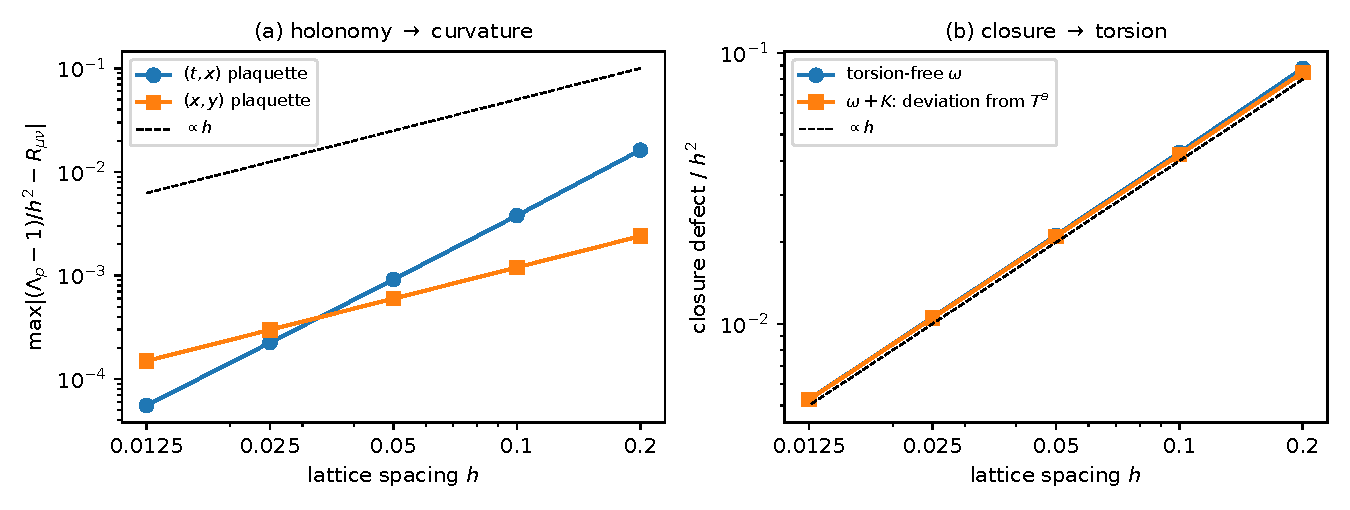
\includegraphics[width=\columnwidth]{fig_cartan_lattice.pdf}
\caption{\label{fig:cartan}Lattice verification of the Cartan structure equations for FLRW,
$a(t)=1+0.3t^2+0.1t^3$, at $x_0=(0.4,0.1,-0.2,0.3)$. (a) Deviation of the plaquette holonomy
$(\Lambda_p-\one)/h^2$ from $R_{\mu\nu}$ at the plaquette center, for the $(t,x)$ and $(x,y)$ planes; it falls as
$h^2$ and $h$, respectively.
(b) Closure defect~\eqref{eq:closure} divided by $h^2$: it vanishes as $O(h)$ for the torsion-free connection, and with
contorsion it converges to the predicted torsion. Reproduced in the companion notebook.}
\end{figure}
%NB:fig1

\subsection{The Einstein--Cartan functional}
\label{sec:ec}

The first gravitational functional we need is linear in curvature. We fix the normalization of the
first-order action in Carroll's conventions.
The notebook verifies, for FLRW with arbitrary $a(t)$, that
$\tfrac12\tilde\epsilon^{\mu\nu\rho\sigma}\epsilon_{abcd}\,e^a{}_\mu e^b{}_\nu R^{cd}{}_{\rho\sigma}=2\sqrt{-g}\,R$ (with
$\tilde\epsilon^{0123}=+1$ and $\epsilon_{0123}=+1$), so that
\begin{equation}
S_{\rm EC}=\frac{1}{32\pi G}\int\epsilon_{abcd}\,e^a\wedge e^b\wedge R^{cd}
=\frac{1}{16\pi G}\int\dd^4x\,\sqrt{-g}\,R .
\label{eq:palatini}
\end{equation}
Using Eqs.~\eqref{eq:dictionary} and~\eqref{eq:holonomy_curvature}, the lattice transcription is
\begin{equation}
\begin{aligned}
S_\Lambda=\frac{1}{64\pi G}\sum_x{}&\tilde\epsilon^{\mu\nu\rho\sigma}\,\epsilon_{abcd}\,
e^a(x,\mu)\,e^b(x,\nu)\\
&\times\big[\Lambda_p(x;\rho\sigma)-\one\big]^{cd},
\end{aligned}
\label{eq:lattice_action}
\end{equation}
which converges to $S_{\rm EC}$ (compare the lattice tetrad formulations of Ref.~\cite{Smolin1979} and the
simplicial formulation of Ref.~\cite{Regge1961}). The notebook confirms that the lattice density converges
linearly in $h$ to $2\sqrt{-g}\,R$. In this functional the holonomy is traced against the
\emph{dual} of the plaquette's area bivector, which is built from edge molecules; this is why it is linear in
$\Lambda_p-\one$. It is the first of the functionals compared in Secs.~\ref{sec:quadratic}
and~\ref{sec:dynamics}.
%NB:palatini

\subsection{Curvature in the spectrum of $\Tc$}
\label{sec:spectral}

The transporters enter the constraint only through $\Tc$. Curvature is therefore visible in the spectral
data that determine the physical states (Theorem~\ref{thm:kernel}).

\begin{proposition}[Spectral detection of curvature]
\label{prop:spectral}
Let $\Gamma$ be connected, with girth (shortest cycle length) $g$, and let $U_{ij}\in\SU$.
\begin{enumerate}
\item[(a)] $\Delta_U$ has a zero mode if and only if the connection is flat, i.e.\ every holonomy is trivial.
\item[(b)] $\tr h^n$ is independent of $U$ for $n<g$, and
\begin{equation}
\tr h^g(U)-\tr h^g(\one)=2g\,(-J)^g\sum_{c}\big(\tr U_c-2\big),
\label{eq:spectral}
\end{equation}
summed over all cycles $c$ of length $g$, with $U_c$ the holonomy around $c$. In particular, the spectrum is gauge invariant.
\end{enumerate}
\end{proposition}
\begin{proof}
(a) $a^\dagger\Delta_Ua=\sum_{\langle ij\rangle}|a_i-U_{ij}a_j|^2=0$ requires $a_i=U_{ij}a_j$ on every link, i.e.\
a covariantly constant spinor, which must be fixed by every holonomy. A nontrivial $\SU$ element has
eigenvalues $e^{\pm i\phi/2}\neq1$ and fixes no nonzero vector. (b) $\tr h^n$ is a sum over closed walks of
length $n$ of products of matrix elements. A walk acquires a nontrivial $U$-dependence only if it
encircles a cycle without retracing, which needs at least $g$ hops. At $n=g$ there are $2g$ such walks per
cycle ($g$ starting points, two orientations), each contributing $(-J)^g\tr U_c$ (the $\SU$ trace is real),
compared with $(-J)^g\tr\one_2$ for $U=\one$.
\end{proof}

For a small rotation angle $\phi_c$, $\tr U_c-2\simeq-\phi_c^2/4$, so the right side of Eq.~\eqref{eq:spectral}
is proportional to Wilson's plaquette action~\cite{Wilson1974,KogutSusskind1975}; more generally, spectral
invariants of covariant Laplacians encode curvature~\cite{Vassilevich2003}. As it stands, however, this
functional weights every plaquette equally. In the continuum it is Yang--Mills theory for the Lorentz group
on the fixed coordinate geometry of the lattice, which is background dependent and is not yet a
gravitational action. Section~\ref{sec:quadratic} shows how weighting by molecular edge data turns it into
one. Curvature also lifts the
bottom of the spectrum of $\Tc$. For a four-cycle with $U_p=e^{-i\theta\sigma_z/2}$,
$\lambda_{\min}(\Delta_U)=2-2\cos(\theta/8)$ (Fig.~\ref{fig:spectrum}). Equation~\eqref{eq:spectral} is checked in
the notebook for a square plaquette with random $\SU$ links, where it reads $8J^4(\tr U_p-2)$ and agrees to
machine precision.

\begin{figure}[t]
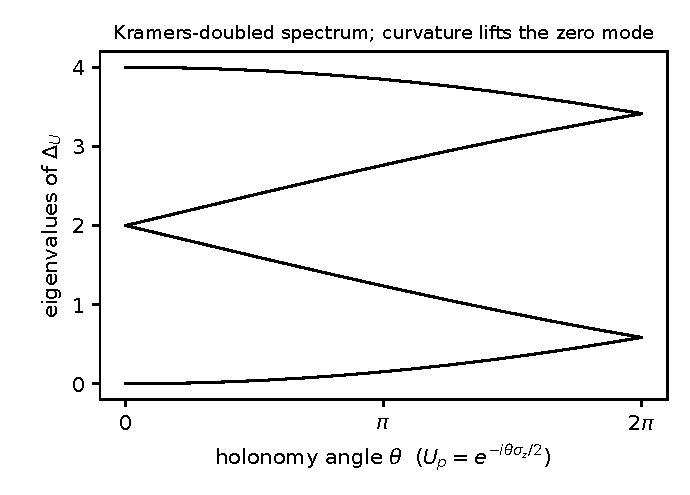
\includegraphics[width=0.92\columnwidth]{fig_spectrum_holonomy.pdf}
\caption{\label{fig:spectrum}Spectrum of the connection Laplacian $\Delta_U$ on a four-cycle as a function of the
holonomy angle $\theta$ ($U_p=e^{-i\theta\sigma_z/2}$). Every level is a Kramers doublet
(Proposition~\ref{prop:kramers}). The zero mode exists only for the flat connection, and curvature lifts it as
$2-2\cos(\theta/8)$ (Proposition~\ref{prop:spectral}). Reproduced in the companion notebook.}
\end{figure}
%NB:spectral

\subsection{Quadratic functionals built from $\Tc$ and the molecules}
\label{sec:quadratic}

The pre-geometry supplies two ingredients for gravitational functionals: the plaquette holonomies
$\Lambda_p$ of the transporters in $\Tc$, and the edge vectors $e^a(x,\mu)$ carried by bond molecules. The
Einstein--Cartan functional~\eqref{eq:lattice_action} is linear in $\Lambda_p-\one$. Traces of holonomies, which
is what the spectrum of $\Tc$ produces (Proposition~\ref{prop:spectral}), are instead quadratic.

\begin{lemma}[Holonomy traces are quadratic in curvature]
\label{lem:trace}
For every plaquette, with no sum over $\mu,\nu$,
\begin{equation}
\begin{aligned}
\tr\Lambda_p(x;\mu\nu)-4&=\tfrac{h^4}{2}\tr\!\big(R_{\mu\nu}R_{\mu\nu}\big)+O(h^5)\\
&=-\tfrac{h^4}{2}\,R^{ab}{}_{\mu\nu}R_{ab\,\mu\nu}+O(h^5).
\end{aligned}
\label{eq:trace_quadratic}
\end{equation}
\end{lemma}
\begin{proof}
By the Baker--Campbell--Hausdorff formula, $\Lambda_p=\exp Z$ with $Z=h^2R_{\mu\nu}+O(h^3)\in\mathfrak{so}(1,3)$. Every
element of $\mathfrak{so}(1,3)$ is traceless, so $\tr e^Z-4=\tfrac12\tr Z^2+O(Z^3)$.
\end{proof}

The linear term is absent, so no trace of a holonomy alone can produce the Einstein--Hilbert density.
Weighting the plaquettes by molecular edge data makes the quadratic functional geometric.
%NB:trace

\begin{proposition}[Metric-weighted holonomy functional]
\label{prop:riem2}
Let $\hat e_a{}^\mu(x)$ be the inverse of the matrix $e^a(x,\mu)/h$, and define the lattice curvature
$\hat R^a{}_{bcd}(x)=\sum_{\mu\nu}\big[(\Lambda_p(x;\mu\nu)-\one)/h^2\big]^a{}_b\,\hat e_c{}^\mu\hat e_d{}^\nu$. Then
\begin{equation}
\begin{aligned}
S_W&\equiv\sum_xh^4\det\!\big[e^a(x,\mu)/h\big]\,\hat R_{abcd}\hat R^{abcd}\\
&\;\longrightarrow\;\int\dd^4x\sqrt{-g}\,R_{abcd}R^{abcd},
\end{aligned}
\label{eq:SW}
\end{equation}
and in four dimensions
\begin{equation}
R_{abcd}R^{abcd}=2\,C_{abcd}C^{abcd}+\tfrac13R^2-E,
\label{eq:riem_decomp}
\end{equation}
with $C_{abcd}$ the Weyl tensor and $E=R_{abcd}R^{abcd}-4R_{ab}R^{ab}+R^2$ the Euler (Gauss--Bonnet) density.
\end{proposition}
\begin{proof}
Convergence follows from Eqs.~\eqref{eq:dictionary} and~\eqref{eq:holonomy_curvature}. In four dimensions
$C_{abcd}C^{abcd}=R_{abcd}R^{abcd}-2R_{ab}R^{ab}+\tfrac13R^2$; eliminating $R_{ab}R^{ab}$ between this and
the definition of $E$ gives Eq.~\eqref{eq:riem_decomp}.
\end{proof}

The notebook verifies Eq.~\eqref{eq:riem_decomp} symbolically for a general static, spherically symmetric
metric with two free functions (where $C^2\neq0$ and $R\neq0$) and for FLRW. It also verifies that the
lattice functional converges linearly in $h$. Since $\int\sqrt{-g}\,E$ is topological in
four dimensions, the metric-weighted holonomy functional is Stelle's quadratic
gravity~\cite{Stelle1977,Stelle1978}, with the Weyl-squared and $R^2$ coefficients in the fixed ratio $6:1$.
%NB:riem2

\begin{proposition}[Chiral holonomy]
\label{prop:chiral}
In the left-atom representation~\eqref{eq:Stheta},
\begin{equation}
\tr S(\theta)S(\theta')=-\tfrac14\,\theta_{ab}\theta'^{ab}+\tfrac{i}{8}\,\epsilon_{abcd}\,\theta^{ab}\theta'^{cd}.
\label{eq:chiral_trace}
\end{equation}
Consequently the metric-weighted density built from the spin-$\tfrac12$ holonomies of the left atoms,
$\tr[S(R_{\mu\nu})S(R^{\mu\nu})]$, has real part $-\tfrac14R_{abcd}R^{abcd}$ and imaginary part proportional to
$\epsilon_{abcd}R^{ab}{}_{ef}R^{cdef}$, the Chern--Pontryagin density, which is a total derivative.
\end{proposition}
\begin{proof}
$S=\tfrac12A^i\sigma_i$ with $A^i$ the self-dual combination of Eq.~\eqref{eq:Stheta}, so
$\tr SS'=\tfrac12A^iA'^i$; the real part of $A^iA'^i$ is $-\tfrac12\theta_{ab}\theta'^{ab}$ and the imaginary part is the
mixed term $\theta_{i0}\epsilon_{ijk}\theta'_{jk}+(\theta\leftrightarrow\theta')$. The coefficients are confirmed by an exact fit in
the companion notebook.
\end{proof}

Chirality therefore does not remove the Weyl-squared term; it adds only a topological imaginary part.
%NB:chiral

\paragraph*{The de Sitter-shifted functional.} The holonomy can also be combined with the molecular area
bivector before squaring. Define
\begin{equation}
F^{ab}=R^{ab}-\tfrac{\Lambda}{3}\,e^a\wedge e^b ,
\label{eq:Fds}
\end{equation}
whose lattice form is $F^{ab}_p=[\Lambda_p-\one]^{ab}/h^2-\tfrac\Lambda3[e(x,\mu)\wedge e(x,\nu)]^{ab}/h^2$.

\begin{proposition}[MacDowell--Mansouri functional]
\label{prop:MM}
With $\tilde\epsilon^{0123}=\epsilon_{0123}=+1$,
\begin{equation}
\tfrac14\tilde\epsilon^{\mu\nu\rho\sigma}\epsilon_{abcd}\,F^{ab}{}_{\mu\nu}F^{cd}{}_{\rho\sigma}
=\sqrt{-g}\,E-\tfrac{4\Lambda}{3}\sqrt{-g}\,\big(R-2\Lambda\big).
\label{eq:MMdensity}
\end{equation}
Hence
\begin{equation}
\begin{aligned}
S_{\rm MM}&\equiv-\frac{3}{64\pi G\Lambda}\int\epsilon_{abcd}\,F^{ab}\wedge F^{cd}\\
&=-\frac{3}{64\pi G\Lambda}\int\dd^4x\sqrt{-g}\,E\\
&\quad+\frac{1}{16\pi G}\int\dd^4x\sqrt{-g}\,(R-2\Lambda),
\end{aligned}
\label{eq:SMM}
\end{equation}
and $F^{ab}$ vanishes identically on de Sitter space with cosmological constant $\Lambda$.
\end{proposition}
\begin{proof}
Expand $F\wedge F$. The $R\wedge R$ term gives $\sqrt{-g}\,E$; the cross term reduces, by the normalization
identity of Eq.~\eqref{eq:palatini}, to $-\tfrac{4\Lambda}{3}\sqrt{-g}\,R$; and the quartic term uses
$\tilde\epsilon^{\mu\nu\rho\sigma}\epsilon_{abcd}e^a{}_\mu e^b{}_\nu e^c{}_\rho e^d{}_\sigma=24\sqrt{-g}$. On de Sitter
space $R^{ab}=\tfrac\Lambda3e^a\wedge e^b$. The notebook verifies Eq.~\eqref{eq:MMdensity} symbolically for FLRW with
arbitrary $a(t)$ and for Schwarzschild--de Sitter, verifies $F\equiv0$ on de Sitter, and verifies convergence
of the lattice density.
\end{proof}

This is the construction of MacDowell and Mansouri~\cite{MacDowellMansouri1977,Wise2010}: a functional
quadratic in a curvature whose only local content is general relativity with a cosmological constant, with
no Weyl-squared term and no scalaron.
%NB:MM

\paragraph*{Spinor form: the atoms as a de Sitter spinor.} In the Dirac representation in a Weyl basis,
$\gamma^a=\left(\begin{smallmatrix}0&\sigma^a\\ \bar\sigma^a&0\end{smallmatrix}\right)$ with
$\sigma^a=(\one,\vec\sigma)$ and $\bar\sigma^a=(-\one,\vec\sigma)$, the Lorentz generators
$S_D(\theta)=\tfrac14\theta_{ab}\gamma^a\gamma^b$ are block diagonal. The lower block is exactly $S(\theta)$ of
Eq.~\eqref{eq:Stheta}, acting on left atoms, and the upper block is $-S(\theta)^\dagger$, the dual of the
right-atom representation. A pair $(\Rat,\Lat)$ is therefore a Dirac spinor. Adding $P_a=\tfrac12\gamma_a\gamma_5$,
the ten generators close into $\mathfrak{so}(4,1)$; the trace form has six negative directions, the compact
$\mathfrak{so}(4)$. The $P_a$ are off diagonal: they convert $\Lat$ into $\Rat$ and back. The connection
\begin{equation}
\mathcal{A}=S_D(\omega)+\ell^{-1}\,e^aP_a,\qquad \Lambda=3/\ell^2 ,
\label{eq:dSconnection}
\end{equation}
is an $\mathfrak{so}(4,1)$ connection whose curvature vanishes identically on de Sitter space. The notebook
checks this directly, and checks that the $\mathfrak{so}(3,2)$ choice $P_a=\tfrac12\gamma_a$ does not vanish
in the companion notebook. Its Lorentz part is the spinor image of Eq.~\eqref{eq:Fds}, and its translational part is the
torsion~\cite{Wise2010}. In the language of this paper, the diagonal blocks of $\mathcal{A}$ are the transporters of
$\Tc$ (self-dual on $\Lat$, anti-self-dual on $\Rat$), and the off-diagonal block is the tetrad: the bond
molecules that connect $\Lat$ to $\Rat$. The MacDowell--Mansouri functional is the quadratic form of the
curvature of this single connection. A caveat applies. The constraint~\eqref{eq:H} conserves
$\hat N_\Lat$ and $\hat N_\Rat$ separately, whereas a quantum implementation of the off-diagonal block requires
chirality-mixing terms such as $a_i^\dagger(e\cdot\sigma)b_j$. These are mirror even and do not commute with
$\sum_i\hat D_i$, so they would break the exact solution of Sec.~\ref{sec:solution}. How to incorporate them is
open.
%NB:desitter

\subsection{Which gravitational dynamics? Quadratic gravity as the natural target}
\label{sec:dynamics}

Everything above holds for any choice of transporters. In the minimal model of Sec.~\ref{sec:wdw} the
$U_{ij}$ are background data; the constraint is then solved exactly, and the kinematic reconstruction of
tetrad, connection, torsion, and curvature goes through. Gravity requires more: the transporters must
become dynamical, and the Wheeler--DeWitt constraint must then select a gravitational action in the
continuum. Four structural results constrain which action that can be.

\begin{proposition}[The constraint has no intrinsic scale]
\label{prop:scale}
For every $\lambda\neq0$, $\ker(\lambda\Hc)=\ker\Hc$. Writing
$\Hc=\epsilon_0\big[\sum_i\hat D_i+(J/\epsilon_0)\sum_{\langle ij\rangle}(\hat B^\Lat_{ij}-\hat B^\Rat_{ij})\big]$, the
physical states depend only on the dimensionless ratio $J/\epsilon_0$ and on the transporters $U_{ij}$.
\end{proposition}

The proof is immediate. The consequence is not. The pre-geometry contains no dimensionful constant, so any
continuum action derived from its physical states can contain dimensionful couplings only through a scale
that is generated dynamically. In four dimensions $\int\sqrt{-g}\,R^2$ and $\int\sqrt{-g}\,C^2$ are dimensionless,
whereas the Einstein--Hilbert and cosmological terms require the dimensionful coefficients $1/G$ and
$\Lambda/G$. \emph{Quadratic gravity is therefore the natural continuum target for this pre-geometry}: it is what a
scale-free microscopic theory can produce with pure-number coefficients, while the linear term must be
induced. Scale invariance is likewise a standard motivation for quadratic gravity~\cite{AlvarezGaume2016}.
%NB:scale

Second, Proposition~\ref{prop:zp} suggests, but does not establish, that the Sakharov route~\cite{Sakharov2000} is closed. The
static vacuum energy of the atoms is independent of $U$. Once the links are dynamical, however, fluctuations of the
two mirror sectors could still generate derivative-dependent terms in an effective action for $U$ and $e$, and deciding
this requires the fluctuation determinants of the dynamical model. If the cancellation does extend to the full
effective action, any gravitational action must come from the \emph{molecular} content of physical states, for example
from condensates such as those of Proposition~\ref{prop:condensate}.

Third, the functionals of Secs.~\ref{sec:ec} and~\ref{sec:quadratic} define three distinct channels, compared in
Table~\ref{tab:channels}.

\begin{table*}[t]
\caption{\label{tab:channels}Gravitational functionals that can be assembled from plaquette holonomies of
$\Tc$ and molecular edge vectors. $E$ is the Euler density and $P$ the Pontryagin density; both are topological.}
\begin{ruledtabular}
\begin{tabular}{lllll}
\parbox[t]{0.12\textwidth}{\raggedright Channel\strut} & \parbox[t]{0.22\textwidth}{\raggedright Molecular origin\strut} & \parbox[t]{0.15\textwidth}{\raggedright Continuum content\strut} & \parbox[t]{0.25\textwidth}{\raggedright Propagating modes\strut} & \parbox[t]{0.18\textwidth}{\raggedright Status\strut} \\
\hline
\parbox[t]{0.12\textwidth}{\raggedright (a) Stelle type\strut} & \parbox[t]{0.22\textwidth}{\raggedright metric-weighted holonomy (Props.~\ref{prop:riem2} and~\ref{prop:chiral})\strut} & \parbox[t]{0.15\textwidth}{\raggedright $2C^2+R^2/3$ (up to $E$ and $iP$)\strut} & \parbox[t]{0.25\textwidth}{\raggedright with an Einstein term: graviton, massive spin-2 ghost,
scalaron~\cite{Stelle1978}\strut} & \parbox[t]{0.18\textwidth}{\raggedright renormalizable~\cite{Stelle1977}; alone, one massive mode is tachyonic (Prop.~\ref{prop:stelle})\strut} \\
\parbox[t]{0.12\textwidth}{\raggedright (b) Starobinsky type\strut} & \parbox[t]{0.22\textwidth}{\raggedright square of the local density in Eq.~\eqref{eq:lattice_action}\strut} & \parbox[t]{0.15\textwidth}{\raggedright $\alpha R+\beta R^2$\strut} & \parbox[t]{0.25\textwidth}{\raggedright graviton and scalaron with $m_f^2=\alpha/6\beta$; no ghost~\cite{AlvarezGaume2016}\strut} & \parbox[t]{0.18\textwidth}{\raggedright inflaton of Sec.~\ref{sec:inflation}~\cite{Starobinsky1980,Planck2018}; $\alpha\neq0$ required\strut} \\
\parbox[t]{0.12\textwidth}{\raggedright (c) MacDowell--Mansouri\strut} & \parbox[t]{0.22\textwidth}{\raggedright $\epsilon$-weighted de Sitter-shifted curvature (Prop.~\ref{prop:MM})\strut} & \parbox[t]{0.15\textwidth}{\raggedright $(R-2\Lambda)/16\pi G$ (up to $E$)\strut} & \parbox[t]{0.25\textwidth}{\raggedright graviton only\strut} & \parbox[t]{0.18\textwidth}{\raggedright GR with $\Lambda$; coefficient
$3/(64\pi G\Lambda)\approx5\times10^{119}$\strut}
\end{tabular}
\end{ruledtabular}
\end{table*}

Fourth, the linear term cannot vanish at low energies. For channel (b), take
$S=(16\pi G_0)^{-1}\int\sqrt{-g}\,f(R)$ with $f(R)=\alpha R+\beta R^2$ and expand about a background of constant curvature
$\bar R$. The tensor kinetic term is multiplied by $f'(\bar R)=\alpha+2\beta\bar R$, so the effective coupling is
$G_{\rm eff}=G_0/f'(\bar R)$. The scalaron mass is
\begin{equation}
m_f^2=\frac13\left(\frac{f'(\bar R)}{f''(\bar R)}-\bar R\right)=\frac{\alpha}{6\beta},
\label{eq:scalaron_mass}
\end{equation}
independent of the background. In the scale-invariant limit $\alpha=0$, the tensor mode propagates only
because $\bar R\neq0$, in agreement with Ref.~\cite{AlvarezGaume2016}: a curved molecular condensate induces the
Einstein term, with $G_{\rm eff}=G_0/(2\beta\bar R)$. But Eq.~\eqref{eq:scalaron_mass} then gives a \emph{massless}
scalaron. Metric $f(R)$ gravity is equivalent to Brans--Dicke theory with $\omega=0$~\cite{SotiriouFaraoni2010}, and a
massless Brans--Dicke scalar gives $\gamma_{\rm PPN}=(1+\omega)/(2+\omega)=\tfrac12$, whereas the Cassini time-delay
measurement gives $\gamma_{\rm PPN}-1=(2.1\pm2.3)\times10^{-5}$~\cite{Bertotti2003}. The Einstein-frame potential of pure
$R^2$ is constant, $(f'R-f)/f'^2=1/4\beta$, so no chameleon-type screening is available. Pure $R^2$ is therefore
excluded as the low-energy theory, and some linear channel, either Eq.~\eqref{eq:lattice_action} or
channel~(c), must survive. Quadratic gravity remains the natural form at the fundamental level; the linear
term is the scale generated by the condensate.
%NB:scalaron

This result connects directly to the Starobinsky-plus-scalar phenomenology of
Ref.~\cite{FarmerLarson2026}. There $f=R(1-\xi\Phi^2)+\beta R^2$, and Eq.~\eqref{eq:scalaron_mass} reproduces the scalaron
mass $m_f^2=(1-\xi\bar\Phi^2)/6\beta$ found in that work, with $\alpha=1-\xi\bar\Phi^2$. In molecular language the scalaron
range $\sqrt{6\beta/\alpha}$ measures the ratio of the quadratic to the linear molecular coefficient. Its observational
bound is discussed in Sec.~\ref{sec:predictions}.

Fifth, channel~(a) cannot stand on its own.

\begin{proposition}[The Stelle-type channel alone is unstable]
\label{prop:stelle}
Let $S=(16\pi G)^{-1}\int\dd^4x\sqrt{-g}\,\big(R+c\,R_{abcd}R^{abcd}\big)$ with $c\neq0$, the Einstein term plus the
metric-weighted holonomy functional of Proposition~\ref{prop:riem2}. The massive scalar and massive spin-2 modes
about flat space have
\begin{equation}
m_0^2=\frac{1}{2c},\qquad m_2^2=-\frac{1}{4c},\qquad\text{so}\qquad m_0^2=-2\,m_2^2 .
\label{eq:stelle_masses}
\end{equation}
For every $c\neq0$ exactly one of the two modes is tachyonic.
\end{proposition}
\begin{proof}
Since $\int\sqrt{-g}\,E$ is topological, $R_{abcd}R^{abcd}\simeq4R_{ab}R^{ab}-R^2$, so the action has the form
$R+aR^2+bR_{ab}R^{ab}$ with $a=-c$ and $b=4c$. For this action the masses are $m_0^2=1/[2(3a+b)]$ and
$m_2^2=-1/b$~\cite{Stelle1978}; the normalization is fixed by the $b=0$ limit, which must reproduce
Eq.~\eqref{eq:scalaron_mass} with $\alpha=1$, i.e.\ $m_0^2=1/6a$. Absence of tachyons requires $3a+b>0$ and
$b<0$, that is, $c>0$ and $c<0$ at once. Equivalently, in the Weyl basis
$R_{abcd}R^{abcd}\simeq2C^2+R^2/3$ [Eq.~\eqref{eq:riem_decomp}], the $R^2$ coefficient $c/3$ and the $C^2$ coefficient
$2c$ have the same sign, whereas stability requires opposite signs.
\end{proof}

A viable quadratic sector therefore cannot consist of holonomy traces alone. It must be dominated by
channels~(b) or~(c), or must include additional terms that change the ratio fixed in Eq.~\eqref{eq:riem_decomp}.
%NB:stelle

In channel~(c) the only coupling is the pure number $3/(64\pi G\Lambda)$, about $5\times10^{119}$ for the observed
$\Lambda$. The cosmological-constant hierarchy thus reappears as the size of a dimensionless
molecular coefficient. The model does not explain it.

The main open problem is now sharply posed. The $U_{ij}$ must be promoted to quantum link variables, in the
manner of Kogut and Susskind~\cite{KogutSusskind1975} and with the corresponding Gauss constraints, and one must
determine which combination of the channels in Table~\ref{tab:channels} the constraint selects: the
coefficients $\alpha$, $\beta$, the Weyl-squared coefficient, and $\Lambda$. A second structural requirement concerns the constraint
itself. $\Hc$ is a sum of local terms but is imposed as a single global constraint, whereas canonical general relativity has
local Hamiltonian and momentum constraints whose algebra is the hypersurface-deformation
algebra~\cite{DeWitt1967,HKT1976}. Refining Eq.~\eqref{eq:H} into local constraints that reproduce this algebra, or otherwise
demonstrating emergent diffeomorphism invariance, is required before the Wheeler--DeWitt interpretation is complete. Two structural hints point to specific
channels. The spectrum of $\Tc$ naturally produces channel~(a). The $\mathfrak{so}(4,1)$ structure of
Eq.~\eqref{eq:dSconnection}, in which the bond molecules are the off-diagonal block, points to channel~(c). In
self-dual language the linear term is $\Sigma_{AB}\wedge F^{AB}$ with $\Sigma^{AB}=e^{A}{}_{A'}\wedge e^{BA'}$ the Pleba\'nski
2-form~\cite{Plebanski1977,JacobsonSmolin1988}, and $\Sigma^{AB}$ is built from the molecular order parameter
$\langle a_Ab_{A'}\rangle$ of two edges meeting at a patch. We therefore \emph{conjecture} that, in molecular-condensate
states, closed-loop transport weighted by the patch bivectors produces the linear term.

%% ======================================================================
\section{De Sitter asymptotics from observation and a dS/CFT completion}
\label{sec:dscft}
%% ======================================================================

Sections~\ref{sec:kinematics}--\ref{sec:geometry} are internal to the model: they construct physical states and
reconstruct geometry, but they do not select a vacuum. The observed universe does. Two facts fix its
asymptotics. First, the expansion is accelerating with an equation of state consistent with a positive
cosmological constant, $\Lambda=3\Omega_\Lambda H_0^2/c^2\simeq1.09\times10^{-52}\,{\rm m}^{-2}$~\cite{Planck2018params}, so the far
future is approximately de Sitter with radius $\ell=\sqrt{3/\Lambda}\simeq1.66\times10^{26}$\,m. Second, the primordial
perturbations are adiabatic, nearly Gaussian, and nearly scale invariant~\cite{Planck2018,Planck2018NG}, the signature
of an earlier quasi-de Sitter phase in its Bunch--Davies state. We take these facts as boundary conditions
instead of deriving them, and we use the dS/CFT correspondence~\cite{Strominger2001,Witten2001,Maldacena2003} to turn
them into a statement about the physical states of Eq.~\eqref{eq:H}. Boundary conditions restrict states; they do
not introduce an ambient spacetime, so background freedom in the sense of Sec.~\ref{sec:background} is unaffected.
Every statement in this section is an exact identity checked in the companion notebook, a postulate imposed by
observation, or a labeled conjecture.

\subsection{The de Sitter boundary condition}

\begin{postulate}[de Sitter asymptotics]
\label{post:ds}
Physical states of Eq.~\eqref{eq:H} are restricted to those whose large-scale geometry, reconstructed as in
Sec.~\ref{sec:geometry}, approaches de Sitter space with the observed $\Lambda$ at late times. Their late-time wave
functional is the partition function of a Euclidean three-dimensional conformal field theory on the future
boundary $\mathcal{I}^+$,
\begin{equation}
\Psi\big[h_{ij},\phi_0\big]=Z_{\rm CFT}\big[h_{ij},\phi_0\big],
\label{eq:dscft}
\end{equation}
where $h_{ij}$ is the conformal class of the late-time spatial metric and $\phi_0$ are the late-time values of the
other fields, which act as sources~\cite{Maldacena2003}.
\end{postulate}

Equation~\eqref{eq:dscft} is the natural partner of a Wheeler--DeWitt constraint: a wave functional with no external
time is identified with a partition function on a spacelike surface. In the canonical reading appropriate to a
Hamiltonian constraint, the graph $\Gamma$ with $\SU$ links is a spatial slice and $\mathcal{I}^+$ is the late-time slice.
This is also why the Fock inner product selects $\SU$ (Sec.~\ref{sec:reality}): it is the rotation group of a
spacelike surface, and, by Corollary~\ref{cor:sitelocal}, the site-local order parameter of a molecular condensate in a
curved region is that surface's timelike normal.

\paragraph*{Where the boundary is.} De Sitter space is conformally flat. In planar coordinates
\begin{equation}
\begin{gathered}
\dd s^2=\Omega(\eta)^2\big(-\dd\eta^2+\delta_{ij}\dd x^i\dd x^j\big),\\
\Omega(\eta)=\ell/(-\eta),\qquad -\infty<\eta<0,
\end{gathered}
\label{eq:dsplanar}
\end{equation}
and $\mathcal{I}^+$ is $\eta\to0^-$. By Corollary~\ref{cor:rigid}, the only geometric datum a patch carries is its conformal
factor $\Omega^2=\sum_{\alpha<\beta}|\omega_{\alpha\beta}|^2$, which measures how strongly its atoms pair. Because the atoms are
fermions, the order parameter carried by one flavor is bounded, $|\langle b\,a\rangle|\le\tfrac12$
(Proposition~\ref{prop:coherent}). The order parameter of a patch, and with it the pairings $\omega_{\alpha\beta}$, grows only with
the number of molecules the patch contains. The future boundary is therefore the limit of divergent pairing,
$\Omega^2\to\infty$: the limit in which each coarse-grained patch of the molecular superfluid holds an unbounded number of
molecules. It is defined by the states of the atoms alone.
%NB:dsbc

\subsection{Boundary conformal symmetry from the atom spinor}

The isometry group of four-dimensional de Sitter space, $SO(4,1)$, acts on $\mathcal{I}^+$ as the conformal group of
three-dimensional Euclidean space. Section~\ref{sec:quadratic} showed that a pair $(\Rat,\Lat)$ carries the Dirac
representation of $\mathfrak{so}(4,1)$, generated by $J_{ab}\equiv S_D(e_{ab})$ and $P_a=\tfrac12\gamma_a\gamma_5$, where
$(e_{ab})_{cd}=\delta_{ac}\delta_{bd}-\delta_{ad}\delta_{bc}$. The atoms therefore carry the boundary conformal algebra.

\begin{proposition}[Boundary conformal algebra]
\label{prop:conformal}
Define, for $i,j\in\{1,2,3\}$,
\begin{equation}
D=P_0,\quad \mathcal{P}_i=J_{0i}+P_i,\quad \mathcal{K}_i=J_{0i}-P_i,\quad M_{ij}=J_{ij}.
\label{eq:confgen}
\end{equation}
Then $[D,\mathcal{P}_i]=\mathcal{P}_i$, $[D,\mathcal{K}_i]=-\mathcal{K}_i$, $[\mathcal{K}_i,\mathcal{P}_j]=2(M_{ij}-\delta_{ij}D)$, and
$[D,M_{ij}]=[\mathcal{P}_i,\mathcal{P}_j]=[\mathcal{K}_i,\mathcal{K}_j]=0$, while $\mathcal{P}_i$ and $\mathcal{K}_i$ transform as vectors under the
rotations $M_{ij}$. This is the conformal algebra of $\mathbb{R}^3$: $D$ is the dilatation, $\mathcal{P}_i$ the translations,
$\mathcal{K}_i$ the special conformal transformations, and $M_{ij}$ the rotations. In the atom representation, $M_{ij}$ is block
diagonal and anti-Hermitian, acting on $\Lat$ and $\Rat$ by the same $\SU$, whereas $D$ is Hermitian and off diagonal,
with eigenvalues $\pm\tfrac12$ on the combinations $\Rat\pm\Lat$ of a single two-spinor.
\end{proposition}
\begin{proof}
Direct computation in the Weyl basis of Sec.~\ref{sec:quadratic}. The notebook verifies every relation exactly.
\end{proof}

Proposition~\ref{prop:conformal} gives each piece of the model a boundary meaning. The rotations of $\mathcal{I}^+$ are the
compact $\SU$ of the transporters in $\Tc$, which treat both species alike. The dilatation is the bulk time
translation $P_0$. It is the one boundary generator that converts $\Lat$ into $\Rat$, and its eigenstates are equal-weight
superpositions of the two species. Bulk evolution toward $\mathcal{I}^+$ is boundary rescaling. This gives a concrete
candidate for the arrow of time left open in Sec.~\ref{sec:audit}: the orientation of information flow ($\Lat$ counted
positive, $\Rat$ negative) corresponds to the direction of scale on the boundary, as in the reading of cosmological
evolution as inverse renormalization-group flow~\cite{Strominger2001b}.
%NB:conformal

\subsection{Physical states as boundary operators}

A bulk spin-$\tfrac12$ field of mass $m$ approaches $\mathcal{I}^+$ as $(-\eta)^{3/2\pm i\mu}$ with $\mu=m\ell$ [Eq.~\eqref{eq:weights}
below], for every $m>0$. In cosmic time, $-\eta=\ell e^{-t/\ell}$, these are $e^{-3t/2\ell}e^{\mp i\mu t/\ell}$: positive and negative
frequency, which the boundary theory records as an operator of weight $\Delta=\tfrac32+i\mu$ and its shadow $3-\Delta=\tfrac32-i\mu$. The mirror sectors of
Eq.~\eqref{eq:Hdiag} have the same structure, with energy $+\epsilon_k$ for $\Lat$ and $-\epsilon_k$ for $\Rat$. This suggests the following
dictionary.

\begin{conjecture}[Shadow dictionary]
\label{conj:shadow}
Under Postulate~\ref{post:ds}, a left atom in normal mode $k$ corresponds to a boundary operator of weight
$\Delta_k=\tfrac32+i\mu_k$, and its mirror partner to the shadow weight $3-\Delta_k=\tfrac32-i\mu_k$, with $\mu_k=\epsilon_k/\epsilon_*$ for a
single constant $\epsilon_*$.
\end{conjecture}
Because the atoms are spin-$\tfrac12$ fermions, the conjecture has the form of the standard spin-$\tfrac12$ entry of the
dictionary, $\mu_k=m_k\ell$, and needs no threshold mass, unlike the scalar case.

If the conjecture holds, the following are exact consequences of Theorem~\ref{thm:kernel} and
Proposition~\ref{prop:zp}.
\begin{enumerate}
\item[(i)] A Fock state $\ket{m,n}$ has total weight $\tfrac32\sum_k(m_k+n_k)+i\sum_k\mu_k(m_k-n_k)$. The constraint
$\Hc\ket\Psi=0$ is the statement that the total weight is real: ${\rm Im}\,\Delta_{\rm tot}=E(m,n)/\epsilon_*=0$.
\item[(ii)] For rationally independent levels the physical states are products of shadow pairs
$\mathcal{O}_{\Delta}\mathcal{O}_{3-\Delta}$ [Theorem~\ref{thm:kernel}(c)]. Each molecule has weight exactly $3$: it is a marginal
operator of the three-dimensional boundary theory, consistent with the absence of an intrinsic scale
(Proposition~\ref{prop:scale}).
\item[(iii)] A state of $r$ molecules has weight $3r$. As a deformation of the boundary theory its coupling scales as
$(-\eta)^{3r-3}$, so every interaction among two or more molecules vanishes at $\mathcal{I}^+$, and faster the more molecules
take part.
\item[(iv)] Zero-point cancellation (Proposition~\ref{prop:zp}) is the statement that the spectrum is symmetric under
$\Delta\leftrightarrow3-\Delta$.
\end{enumerate}
The conjecture is not derived here. The notebook checks only that it is consistent with the exact solution: the
states of real total weight are exactly the kernel of $\Hc$ in Table~\ref{tab:balance}.
%NB:shadow

\subsection{The cosmological constant as a count of boundary degrees of freedom}

In dS/CFT the number of boundary degrees of freedom scales as $\ell^2/G$~\cite{Strominger2001}, the combination that
sets the Gibbons--Hawking entropy $S_{\rm dS}=A/4G=\pi\ell^2/G$~\cite{GibbonsHawking1977}. The pure-number coefficient of
channel~(c) is exactly this entropy:
\begin{equation}
\frac{3}{64\pi G\Lambda}=\frac{S_{\rm dS}}{64\pi^2},\qquad S_{\rm dS}=\frac{3\pi}{G\Lambda}\simeq3.3\times10^{122}
\label{eq:entropy}
\end{equation}
(with $\hbar=c=1$). The large number of Sec.~\ref{sec:dynamics} is therefore the de Sitter entropy, and the observed
cosmological constant is $\Lambda=3\pi/(GS_{\rm dS})$: the inverse of the number of boundary degrees of freedom. Because
the atoms carry no zero-point energy (Proposition~\ref{prop:zp}), $\Lambda$ is not a vacuum energy of the pre-geometry.
This does not explain why $S_{\rm dS}$ is so large, and it does not remove the vacuum energy of matter fields: with
Postulate~\ref{post:ds} imposed, the matter contribution is part of the observed value.
%NB:entropy

\subsection{Matter: the Standard Model on the molecular network}

\paragraph*{Coupling principle.} By Eq.~\eqref{eq:Stheta}, a left atom transforms under the self-dual half of a Lorentz
transformation and a right atom under the anti-self-dual half. Every left-handed Weyl field of the Standard Model
transforms the same way, as $(\tfrac12,0)$, and every right-handed field as $(0,\tfrac12)$; like the atoms, these fields are
fermions. Standard-Model fermions therefore couple to the emergent geometry through the transporters of $\Tc$ themselves: a left-handed field on
patch $j$ is carried to patch $i$ by $U_{ij}$, and a right-handed field by $\bar U_{ij}$ (by the $\SLC$ transporters of
Sec.~\ref{sec:geometry} once boosts are included). Gauge fields enter as additional internal link variables
$W_{ij}\in SU(3)\times SU(2)_{\rm W}\times U(1)_Y$ on the same graph, in the Kogut--Susskind form~\cite{KogutSusskind1975}, and the
Higgs doublet as a site variable. The minimal model does not fix the gauge group, the representations, or the
number of generations, and nothing in it conflicts with them. The chiral structure of the Standard Model,
left-handed doublets and right-handed singlets, uses exactly the two Lorentz representations carried by $\Lat$
and $\Rat$.

\paragraph*{Boundary content.} Under Postulate~\ref{post:ds} each bulk field maps to boundary operators whose weights
follow from its mass and spin. For a scalar and a spin-$\tfrac12$ field,
\begin{equation}
\Delta_\pm=\tfrac32\pm\sqrt{\tfrac94-m^2\ell^2}\quad\text{and}\quad\Delta_\pm=\tfrac32\pm im\ell ,
\label{eq:weights}
\end{equation}
respectively. Massless gauge fields give conserved currents with $\Delta=2$, and the graviton gives the boundary stress
tensor with $\Delta=3$. Table~\ref{tab:sm} lists the Standard-Model content at the two de Sitter epochs. Among the asymptotic
late-time states, only the graviton and the photon give real weights, so unbroken $U(1)_{\rm em}$ is a global symmetry
of the boundary theory. Every massive particle appears as a principal-series pair with
$\mu\simeq m\ell$, between $10^{31}$ (neutrinos) and $10^{44}$ (top quark); the spin-dependent corrections to $\mu$ are
negligible at these values. During inflation (Sec.~\ref{sec:inflation}) every Standard-Model mass is more than ten orders of
magnitude below the Hubble rate, so fermions and gauge fields are nearly conformal. Complex weights make the
boundary theory non-unitary, as expected for de Sitter duals~\cite{Strominger2001,AHS2017}. The best-studied explicit
example, the $Sp(N)$ model dual to higher-spin gravity in de Sitter space, uses anticommuting scalars~\cite{AHS2017}, a
boundary theory in which spin and statistics are not tied together. In the bulk model of this paper, by contrast, the
atoms obey the usual connection between spin and statistics.

\begin{table*}[t]
\caption{\label{tab:sm}Standard-Model and gravitational fields mapped to boundary operators under
Postulate~\ref{post:ds}, using Eq.~\eqref{eq:weights}. Late times: $\ell=\sqrt{3/\Lambda}=1.66\times10^{26}$\,m, and $\mu\simeq m\ell$ for every
massive field. Inflation: the $R^2$ inflaton of Sec.~\ref{sec:inflation} with $N=55$, $H_{\rm inf}=1.6\times10^{13}$\,GeV, using
present-day masses. Masses from Ref.~\cite{PDG2024}; the neutrino entry uses the atmospheric mass splitting as a
lower bound on the heaviest neutrino mass. Weights are free-field values. For unstable or confined fields they
label the corresponding boundary operators in the free limit; the asymptotic late-time states are gravitons,
photons, and the stable massive particles.}
\begin{ruledtabular}
\begin{tabular}{llllll}
\parbox[t]{0.17\textwidth}{\raggedright Field\strut} & \parbox[t]{0.05\textwidth}{\raggedright Spin\strut} & \parbox[t]{0.14\textwidth}{\raggedright Mass\strut} & \parbox[t]{0.25\textwidth}{\raggedright Operator at $\mathcal{I}^+$\strut} & \parbox[t]{0.18\textwidth}{\raggedright Weight at $\mathcal{I}^+$\strut} & \parbox[t]{0.11\textwidth}{\raggedright $m/H_{\rm inf}$\strut} \\
\hline
\parbox[t]{0.17\textwidth}{\raggedright graviton\strut} & \parbox[t]{0.05\textwidth}{\raggedright 2\strut} & \parbox[t]{0.14\textwidth}{\raggedright 0\strut} & \parbox[t]{0.25\textwidth}{\raggedright stress tensor $T_{ij}$\strut} & \parbox[t]{0.18\textwidth}{\raggedright $3$\strut} & \parbox[t]{0.11\textwidth}{\raggedright $0$\strut} \\
\parbox[t]{0.17\textwidth}{\raggedright photon\strut} & \parbox[t]{0.05\textwidth}{\raggedright 1\strut} & \parbox[t]{0.14\textwidth}{\raggedright 0\strut} & \parbox[t]{0.25\textwidth}{\raggedright conserved current $J_i^{\rm em}$\strut} & \parbox[t]{0.18\textwidth}{\raggedright $2$\strut} & \parbox[t]{0.11\textwidth}{\raggedright $0$\strut} \\
\parbox[t]{0.17\textwidth}{\raggedright gluons\strut} & \parbox[t]{0.05\textwidth}{\raggedright 1\strut} & \parbox[t]{0.14\textwidth}{\raggedright 0 (confined)\strut} & \parbox[t]{0.25\textwidth}{\raggedright $SU(3)$ currents (free limit)\strut} & \parbox[t]{0.18\textwidth}{\raggedright $2$\strut} & \parbox[t]{0.11\textwidth}{\raggedright $0$\strut} \\
\parbox[t]{0.17\textwidth}{\raggedright neutrino $\nu_3$\strut} & \parbox[t]{0.05\textwidth}{\raggedright $\tfrac12$\strut} & \parbox[t]{0.14\textwidth}{\raggedright $\geq0.050$\,eV\strut} & \parbox[t]{0.25\textwidth}{\raggedright principal series\strut} & \parbox[t]{0.18\textwidth}{\raggedright $\tfrac32\pm i\,4.2\times10^{31}$\strut} & \parbox[t]{0.11\textwidth}{\raggedright $3\times10^{-24}$\strut} \\
\parbox[t]{0.17\textwidth}{\raggedright electron\strut} & \parbox[t]{0.05\textwidth}{\raggedright $\tfrac12$\strut} & \parbox[t]{0.14\textwidth}{\raggedright $0.511$\,MeV\strut} & \parbox[t]{0.25\textwidth}{\raggedright principal series\strut} & \parbox[t]{0.18\textwidth}{\raggedright $\tfrac32\pm i\,4.3\times10^{38}$\strut} & \parbox[t]{0.11\textwidth}{\raggedright $3\times10^{-17}$\strut} \\
\parbox[t]{0.17\textwidth}{\raggedright $W$, $Z$\strut} & \parbox[t]{0.05\textwidth}{\raggedright 1\strut} & \parbox[t]{0.14\textwidth}{\raggedright $80.4$, $91.2$\,GeV\strut} & \parbox[t]{0.25\textwidth}{\raggedright principal series\strut} & \parbox[t]{0.18\textwidth}{\raggedright $\tfrac32\pm i\,6.8\times10^{43}$, $\tfrac32\pm i\,7.7\times10^{43}$\strut} & \parbox[t]{0.11\textwidth}{\raggedright $5\times10^{-12}$, $6\times10^{-12}$\strut} \\
\parbox[t]{0.17\textwidth}{\raggedright Higgs\strut} & \parbox[t]{0.05\textwidth}{\raggedright 0\strut} & \parbox[t]{0.14\textwidth}{\raggedright $125.2$\,GeV\strut} & \parbox[t]{0.25\textwidth}{\raggedright principal series\strut} & \parbox[t]{0.18\textwidth}{\raggedright $\tfrac32\pm i\,1.1\times10^{44}$\strut} & \parbox[t]{0.11\textwidth}{\raggedright $8\times10^{-12}$\strut} \\
\parbox[t]{0.17\textwidth}{\raggedright top quark\strut} & \parbox[t]{0.05\textwidth}{\raggedright $\tfrac12$\strut} & \parbox[t]{0.14\textwidth}{\raggedright $172.6$\,GeV\strut} & \parbox[t]{0.25\textwidth}{\raggedright principal series\strut} & \parbox[t]{0.18\textwidth}{\raggedright $\tfrac32\pm i\,1.5\times10^{44}$\strut} & \parbox[t]{0.11\textwidth}{\raggedright $1\times10^{-11}$\strut} \\
\parbox[t]{0.17\textwidth}{\raggedright scalaron (inflaton)\strut} & \parbox[t]{0.05\textwidth}{\raggedright 0\strut} & \parbox[t]{0.14\textwidth}{\raggedright $3.1\times10^{13}$\,GeV\strut} & \parbox[t]{0.25\textwidth}{\raggedright principal series\strut} & \parbox[t]{0.18\textwidth}{\raggedright $\tfrac32\pm i\,2.6\times10^{55}$\strut} & \parbox[t]{0.11\textwidth}{\raggedright slow roll\strut}
\end{tabular}
\end{ruledtabular}
\end{table*}
%NB:smtable

\subsection{Inflation as an earlier de Sitter phase}
\label{sec:inflation}

The second observational boundary condition, nearly scale-invariant primordial perturbations, is met by channels
already present. Combining channels~(b) and~(c),
\begin{equation}
S=\frac{1}{16\pi G}\int\dd^4x\sqrt{-g}\left(R-2\Lambda+\frac{R^2}{6M^2}\right),
\label{eq:starobinsky}
\end{equation}
which is Eq.~\eqref{eq:scalaron_mass} with $\alpha=1$ and $\beta=1/6M^2$, so $m_f=M$. The scalaron is the inflaton of Starobinsky's
model~\cite{Starobinsky1980,MukhanovChibisov1981}. In the Einstein frame its potential is
$V=\tfrac34M^2M_P^2\big(1-e^{-\sqrt{2/3}\,\phi/M_P}\big)^2$, with $M_P=(8\pi G)^{-1/2}$, and slow roll gives, to leading order in $1/N$,
\begin{equation}
n_s\simeq1-\frac2N,\qquad r\simeq\frac{12}{N^2},\qquad A_s\simeq\frac{N^2M^2}{24\pi^2M_P^2},
\label{eq:staro_obs}
\end{equation}
where $N$ is the number of $e$-folds between horizon exit of the pivot scale and the end of inflation. The measured
amplitude $A_s\simeq2.1\times10^{-9}$~\cite{Planck2018params} fixes $M\simeq3.1\times10^{13}$\,GeV and $H_{\rm inf}\simeq M/2$ for $N=55$. Three
consistency checks follow. First, the coefficient of $R^2$ in Eq.~\eqref{eq:starobinsky} is the pure number
\begin{equation}
\frac{\beta}{16\pi G}=\frac{M_P^2}{12M^2}=\frac{N^2}{288\pi^2A_s}\simeq5\times10^{8},
\label{eq:R2coef}
\end{equation}
as Proposition~\ref{prop:scale} requires of a quadratic coefficient. Second, $\beta/\alpha=1/6M^2\simeq7\times10^{-60}\,{\rm m}^2$, some fifty
orders of magnitude below the laboratory bound~\eqref{eq:beta_bound}, so the inflaton is the scalaron of P3 and leaves
P1--P4 of Sec.~\ref{sec:predictions} unchanged. Third, in dS/CFT the inflationary phase is a second, approximate de
Sitter boundary~\cite{Strominger2001b}, with entropy $S_{\rm inf}=8\pi^2M_P^2/H_{\rm inf}^2\simeq2\times10^{12}$. Between the two epochs the
number of boundary degrees of freedom grows by a factor of about $10^{110}$, the direction required if cosmological time
is inverse renormalization-group flow on the boundary~\cite{Strominger2001b}.
%NB:inflation

%% ======================================================================
\section{Observational consequences}
\label{sec:predictions}
%% ======================================================================

The model is not yet complete enough to predict the values of $\alpha$, $\beta$, or $\Lambda$ from first principles.
It does make structural statements that can be confronted with observation, and it converts existing bounds
into constraints on its molecular coefficients. We list them in order of robustness and summarize them in
Table~\ref{tab:predictions}. None of them is unique to this model taken singly; together they are the
conditions any completion must satisfy, and each would falsify a specific part of the construction if
violated.

\paragraph*{P1. Luminal tensor waves.} In every channel the massless spin-2 mode propagates on the light cone of
the single emergent metric, the light cone built from the atom pairing (Proposition~\ref{prop:tetrad}). The
gravitational and electromagnetic light cones therefore coincide. GW170817 and GRB~170817A bound the
fractional difference between the speeds of gravity and light to lie between $-3\times10^{-15}$ and
$+7\times10^{-16}$~\cite{GW170817GRB}. A violation would falsify the identification of the gravitational light cone
with the atomic one.

\paragraph*{P2. No long-range scalar.} The scale-invariant limit $\alpha=0$ gives a massless scalaron and
$\gamma_{\rm PPN}=\tfrac12$ (Sec.~\ref{sec:dynamics}), in conflict with the Cassini bound
$\gamma_{\rm PPN}-1=(2.1\pm2.3)\times10^{-5}$~\cite{Bertotti2003}. The model therefore requires an induced linear term,
$\alpha\neq0$. With $\alpha\neq0$ and a scalaron range far below solar-system distances it predicts
$\gamma_{\rm PPN}=1$ there~\cite{Berry2011}.

\paragraph*{P3. A short-range scalaron.} In channel~(b) the scalaron adds a Yukawa term of strength $\tfrac13$ and
range $\lambda_f=m_f^{-1}=\sqrt{6\beta/\alpha}$ to the Newtonian potential~\cite{Stelle1978,Berry2011}. Torsion-balance
tests of the inverse-square law exclude gravitational-strength Yukawa interactions with ranges above
$38.6\,\mu$m~\cite{Lee2020}. For the strength-$\tfrac13$ scalaron of $f=R+a_2R^2/2$, earlier E\"ot-Wash data give
$|a_2|\lesssim2\times10^{-9}\,{\rm m}^2$, i.e.\ $\lambda_f=\sqrt{3a_2}\lesssim8\times10^{-5}$\,m~\cite{Berry2011}; the newer data of
Ref.~\cite{Lee2020} can only tighten this, and we use the conservative value. Since $\beta/\alpha=a_2/2$, this becomes
\begin{equation}
\frac{\beta}{\alpha}=\frac{\lambda_f^2}{6}\lesssim1\times10^{-9}\ {\rm m}^2 ,
\label{eq:beta_bound}
\end{equation}
a bound on the ratio of the quadratic to the linear molecular coefficient. The scalar (breathing)
polarization can propagate only above the angular frequency $\omega_c=c/\lambda_f\gtrsim3.7\times10^{12}\,{\rm s}^{-1}$, so it is
not excited by astrophysical sources~\cite{Berry2011}. The scalaron mass $1/6\beta$ is fixed by the action rather
than by the environment, so the model supplies no screening. Analyses of $R+\beta R^2$ gravity that use $\beta$ far
above Eq.~\eqref{eq:beta_bound}, such as the pulsar-motivated scales of Ref.~\cite{FarmerLarson2026}, therefore
implicitly require the scalaron to be screened or decoupled from laboratory matter; within the molecular
model no such mechanism has been identified.

\paragraph*{P4. Exactly two polarizations at detector frequencies.} Combining P1--P3: in channel~(c) the only
propagating mode is the massless graviton, and in channel~(b) the scalaron lies above the cutoff of P3.
LISA and ground-based detectors should see exactly the two tensor polarizations of general relativity, with
no scalar component and no dispersion. Channel~(a) alone is excluded by Proposition~\ref{prop:stelle}; its massive
spin-2 mode would in addition be bounded by the same torsion-balance tests, since it contributes a Yukawa
term of strength $-\tfrac43$~\cite{Stelle1978}.

\paragraph*{P5. The atomic vacuum does not gravitate.} Zero-point energies cancel identically between the mirror
sectors (Proposition~\ref{prop:zp}), so the pre-geometry contributes no static vacuum energy; whether it also induces no
Sakharov-type action is open. The cosmological constant enters only through the coefficient of channel~(c), the pure
number $3/(64\pi G\Lambda)\approx5\times10^{119}$, which under Postulate~\ref{post:ds} is the de Sitter entropy divided by $64\pi^2$
[Eq.~\eqref{eq:entropy}]. The model relocates the cosmological-constant problem to the size of this number; it does
not solve it.

\paragraph*{P6. Starobinsky tilt and tensor amplitude.} Equation~\eqref{eq:staro_obs} gives $n_s=0.960$--$0.967$ and
$r=0.0048$--$0.0033$ for $N=50$--$60$ (Fig.~\ref{fig:nsr}). CMB data alone give $n_s=0.9682\pm0.0032$ and $r<0.034$ at 95\%
confidence (Planck, SPT, ACT, and BICEP/Keck combined~\cite{Balkenhol2026}), consistent with the prediction for $N\gtrsim55$
(within $1.4\sigma$; $2.6\sigma$ at $N=50$). Adding
DESI DR2 BAO raises the tilt to $n_s=0.9728\pm0.0029$~\cite{Balkenhol2026}, and the Planck--ACT--DESI DR1 combination gives
$0.974\pm0.003$~\cite{ACTDR6}; the former places the prediction $2.1\sigma$ ($N=60$) to $4.4\sigma$ ($N=50$) low. Whether the shift reflects inflationary
physics or an inconsistency between BAO and CMB data is debated~\cite{Ferreira2026}. The decisive test is $r$. LiteBIRD
targets $\delta r<0.001$~\cite{LiteBIRD2023}, enough to detect $r=0.0033$--$0.0048$ at 3--5$\sigma$; its launch is now planned
for the 2030s~\cite{LiteBIRDJAXA}, and ground-based polarization experiments will tighten the bound on $r$ in the meantime. A detection of $r\gtrsim0.01$, or a
bound $r<0.002$, would exclude the $R^2$ channel as the inflaton.

\paragraph*{P7. A cosmological constant, not dynamical dark energy.} Postulate~\ref{post:ds} in its minimal form, with $\Lambda$
supplied by channel~(c), requires $w=-1$ at all late times. DESI DR2 BAO combined with the CMB prefers evolving dark
energy at $3.1\sigma$, and at 2.8--4.2$\sigma$ when supernova samples are added~\cite{DESIDR2}. Confirmation at high significance
would require replacing the constant $\Lambda$ of channel~(c) by a dynamical sector and would remove the exact de Sitter
future on which Eq.~\eqref{eq:dscft} rests.

\paragraph*{P8. Single-field consistency.} With Bunch--Davies initial conditions, the squeezed bispectrum of a
single-field model is fixed by the tilt, $f_{\rm NL}^{\rm local}=\tfrac{5}{12}(1-n_s)\simeq0.015$~\cite{Maldacena2003}. In dS/CFT this
relation is a Ward identity of the boundary conformal symmetry. Planck gives $f_{\rm NL}^{\rm local}=-0.9\pm5.1$~\cite{Planck2018NG},
and SPHEREx, launched in 2025, targets an uncertainty of order unity~\cite{SPHEREx2026}. A detection of
$|f_{\rm NL}^{\rm local}|\gtrsim1$ would exclude the single-scalaron picture.

\begin{table*}[t]
\caption{\label{tab:predictions}Observational consequences of the model and their status.}
\begin{ruledtabular}
\begin{tabular}{llll}
\parbox[t]{0.04\textwidth}{\raggedright \strut} & \parbox[t]{0.30\textwidth}{\raggedright Model statement\strut} & \parbox[t]{0.36\textwidth}{\raggedright Observation\strut} & \parbox[t]{0.22\textwidth}{\raggedright Status\strut} \\
\hline
\parbox[t]{0.04\textwidth}{\raggedright P1\strut} & \parbox[t]{0.30\textwidth}{\raggedright massless tensor modes travel on the atomic light cone\strut} & \parbox[t]{0.36\textwidth}{\raggedright $-3\times10^{-15}<\Delta v/c<7\times10^{-16}$ (GW170817)~\cite{GW170817GRB}\strut} & \parbox[t]{0.22\textwidth}{\raggedright consistent\strut} \\
\parbox[t]{0.04\textwidth}{\raggedright P2\strut} & \parbox[t]{0.30\textwidth}{\raggedright pure $R^2$ ($\alpha=0$) gives $\gamma_{\rm PPN}=\tfrac12$; $\alpha\neq0$ required\strut} & \parbox[t]{0.36\textwidth}{\raggedright $\gamma_{\rm PPN}-1=(2.1\pm2.3)\times10^{-5}$ (Cassini)~\cite{Bertotti2003}\strut} & \parbox[t]{0.22\textwidth}{\raggedright pure $R^2$ excluded\strut} \\
\parbox[t]{0.04\textwidth}{\raggedright P3\strut} & \parbox[t]{0.30\textwidth}{\raggedright scalaron: Yukawa strength $\tfrac13$, range $\sqrt{6\beta/\alpha}$\strut} & \parbox[t]{0.36\textwidth}{\raggedright $\lambda_f\lesssim8\times10^{-5}$\,m (torsion balance)~\cite{Berry2011,Lee2020}\strut} & \parbox[t]{0.22\textwidth}{\raggedright $\beta/\alpha\lesssim1\times10^{-9}$\,m$^2$\strut} \\
\parbox[t]{0.04\textwidth}{\raggedright P4\strut} & \parbox[t]{0.30\textwidth}{\raggedright two tensor polarizations at detector frequencies\strut} & \parbox[t]{0.36\textwidth}{\raggedright scalar cutoff $\omega_c\gtrsim3.7\times10^{12}$\,s$^{-1}$~\cite{Berry2011}\strut} & \parbox[t]{0.22\textwidth}{\raggedright testable (LIGO, LISA)\strut} \\
\parbox[t]{0.04\textwidth}{\raggedright P5\strut} & \parbox[t]{0.30\textwidth}{\raggedright no vacuum energy from the atoms\strut} & \parbox[t]{0.36\textwidth}{\raggedright $\Lambda$ set by a pure number $\approx5\times10^{119}=S_{\rm dS}/64\pi^2$\strut} & \parbox[t]{0.22\textwidth}{\raggedright not explained\strut} \\
\parbox[t]{0.04\textwidth}{\raggedright P6\strut} & \parbox[t]{0.30\textwidth}{\raggedright $n_s\simeq1-2/N$, $r\simeq12/N^2$ ($R^2$ inflaton)\strut} & \parbox[t]{0.36\textwidth}{\raggedright $n_s=0.9682\pm0.0032$, $r<0.034$ (CMB)~\cite{Balkenhol2026}; $n_s=0.9728\pm0.0029$ (CMB+BAO)~\cite{Balkenhol2026}\strut} & \parbox[t]{0.22\textwidth}{\raggedright consistent for $N\gtrsim55$ (CMB); 2.1--4.4$\sigma$ low (CMB+BAO); LiteBIRD decisive\strut} \\
\parbox[t]{0.04\textwidth}{\raggedright P7\strut} & \parbox[t]{0.30\textwidth}{\raggedright $w=-1$ exactly\strut} & \parbox[t]{0.36\textwidth}{\raggedright evolving dark energy preferred at 2.8--4.2$\sigma$ (DESI DR2)~\cite{DESIDR2}\strut} & \parbox[t]{0.22\textwidth}{\raggedright under pressure\strut} \\
\parbox[t]{0.04\textwidth}{\raggedright P8\strut} & \parbox[t]{0.30\textwidth}{\raggedright $f_{\rm NL}^{\rm local}=\tfrac5{12}(1-n_s)\simeq0.015$\strut} & \parbox[t]{0.36\textwidth}{\raggedright $-0.9\pm5.1$ (Planck)~\cite{Planck2018NG}; SPHEREx $\sigma\sim1$\strut} & \parbox[t]{0.22\textwidth}{\raggedright consistent; testable\strut}
\end{tabular}
\end{ruledtabular}
\end{table*}

\begin{figure}[t]
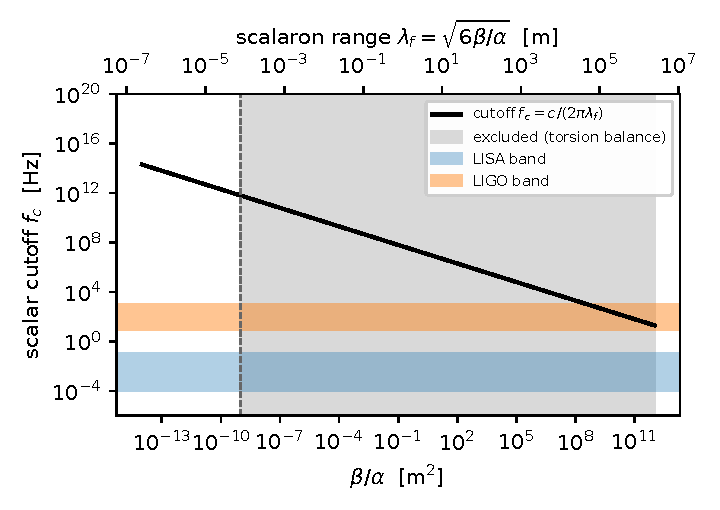
\includegraphics[width=\columnwidth]{fig_scalaron_bounds.pdf}
\caption{\label{fig:scalaron}Cutoff frequency $f_c=c/(2\pi\lambda_f)$ of the scalar polarization as a function of $\beta/\alpha$
(bottom axis) and of the scalaron range $\lambda_f=\sqrt{6\beta/\alpha}$ (top axis). The shaded region
is excluded by torsion-balance tests ($\lambda_f\gtrsim8\times10^{-5}$\,m). Horizontal bands mark the LISA and LIGO
frequency ranges: throughout the allowed region the scalar cutoff lies many orders of magnitude above both.
Reproduced in the companion notebook.}
\end{figure}
%NB:predictions

\begin{figure}[t]
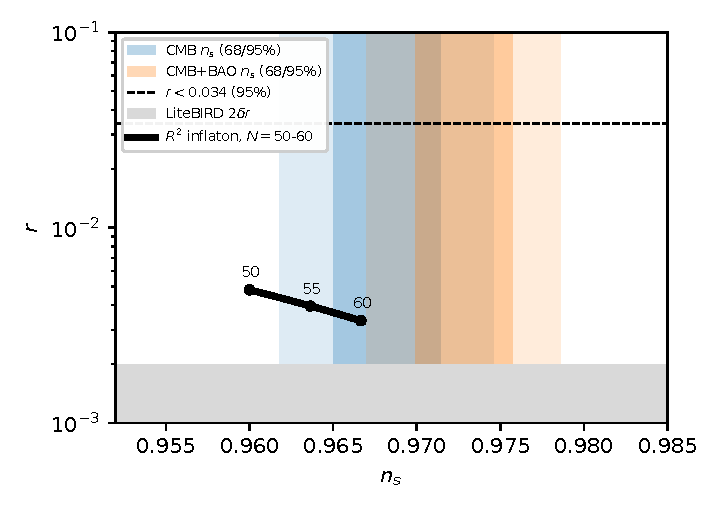
\includegraphics[width=\columnwidth]{fig_ns_r.pdf}
\caption{\label{fig:nsr}Prediction P6 of the $R^2$ inflaton, $n_s\simeq1-2/N$ and $r\simeq12/N^2$ for $N=50$--$60$ (thick line; dots at
$N=50,55,60$), against one-dimensional data intervals (not joint contours): the tilt from CMB data alone,
$0.9682\pm0.0032$, and from CMB plus DESI DR2 BAO, $0.9728\pm0.0029$ (68\% and 95\% bands)~\cite{Balkenhol2026}; the 95\% upper
limit $r<0.034$~\cite{Balkenhol2026}; and the LiteBIRD target $\delta r=0.001$~\cite{LiteBIRD2023}. Reproduced in the companion
notebook.}
\end{figure}
%NB:cmbtests

%% ======================================================================
\section{Formal verification in Lean 4 and Rocq}
\label{sec:lean}
%% ======================================================================

The algebraic results of this paper are machine-checked in two proof assistants with different logical
foundations and independent kernels: Lean~4~\cite{Lean4} (\texttt{MolecularWDW.lean}) and Rocq, formerly
Coq~\cite{Rocq} (\texttt{MolecularWDW.v}). A single proof assistant certifies a proof relative to its own kernel and
encoding; a second, independent formalization guards against errors in either. The two files were written
separately from the informal statements and use different encodings. Both construct the fermionic ladder
operators on the occupation basis, with each mode empty or singly occupied, and Jordan--Wigner signs for the
mode-interleaved ordering $\prod_k(c_k^\dagger)^{m_k}(d_k^\dagger)^{n_k}\ket0$. Lean indexes normal modes by \texttt{Fin K},
computes the signs from finite sums, and proves polynomial identities over the integers; this implies them in every
commutative ring, since an integer-coefficient identity that holds for all integer arguments is an identity of
polynomials. Rocq stores occupations in Boolean lists, computes the signs from prefix counts, and proves polynomial
identities over an arbitrary commutative ring.
Both use only their standard libraries. Table~\ref{tab:formal} maps each formalized result to its theorem in each
file.

\paragraph*{Trusted base.} In Lean, every theorem depends at most on the three standard axioms
\texttt{propext}, \texttt{Quot.sound}, and \texttt{Classical.choice}; the conformal-algebra computations depend on
none. In Rocq, every statement about the exact solution, the spinor identities, and the conformal algebra is
closed under the global context, that is, it uses no axioms at all. The six real-number identities use only
the two axioms of Rocq's real-number library (\texttt{sig\_forall\_dec} and \texttt{functional\_extensionality\_dep}).
Neither file contains \texttt{sorry}, \texttt{admit}, or \texttt{Admitted}, and each prints the assumptions of every main
theorem. Both build in one to two minutes: \texttt{lean MolecularWDW.lean} (Lean~4.15.0) and \texttt{coqc
MolecularWDW.v} (Coq~8.18.0).

\begin{table*}[t]
\caption{\label{tab:formal}Results formalized in both proof assistants. Normalizations: Eq.~\eqref{eq:etaeps} uses the
unnormalized soldering $\tilde\Mol=\Mol^0\one+\Mol^i\sigma_i$ (factor 2); Eq.~\eqref{eq:chiral_trace} is multiplied by 16;
Proposition~\ref{prop:conformal} uses the generators multiplied by 2; Theorem~\ref{thm:kernel}(c) is formalized for
nondegenerate modes; the Lean forms of Eqs.~\eqref{eq:scalaron_mass}--\eqref{eq:R2coef} are cleared of denominators, the
Rocq forms are stated over $\mathbb{R}$.}
\begin{ruledtabular}
\begin{tabular}{lll}
\parbox[t]{0.36\textwidth}{\raggedright Result\strut} & \parbox[t]{0.30\textwidth}{\raggedright Lean 4 theorem\strut} & \parbox[t]{0.30\textwidth}{\raggedright Rocq theorem\strut} \\
\hline
\parbox[t]{0.36\textwidth}{\raggedright anticommutation relations $\{c_k,c^\dagger_l\}=\delta_{kl}$, $\{d_k,d^\dagger_k\}=1$; Pauli principle, Prop.~\ref{prop:hardcore}(a)\strut} & \parbox[t]{0.30\textwidth}{\raggedright \texttt{car\_c}, \texttt{c\_cdag\_anticomm}, \texttt{car\_d}, \texttt{pauli\_c}\strut} & \parbox[t]{0.30\textwidth}{\raggedright same names\strut} \\
\parbox[t]{0.36\textwidth}{\raggedright atoms anticommute: $c^\dagger c^\dagger$, $d^\dagger d^\dagger$, $c^\dagger d^\dagger$, Prop.~\ref{prop:hardcore}(a)\strut} & \parbox[t]{0.30\textwidth}{\raggedright \texttt{cdag\_anticomm}, \texttt{ddag\_anticomm}, \texttt{cdag\_ddag\_anticomm}\strut} & \parbox[t]{0.30\textwidth}{\raggedright same names\strut} \\
\parbox[t]{0.36\textwidth}{\raggedright molecules are bosons, Prop.~\ref{prop:hardcore}(b)\strut} & \parbox[t]{0.30\textwidth}{\raggedright \texttt{molecules\_commute}, \texttt{molecule\_atom\_comm\_c}, \texttt{molecule\_atom\_comm\_d}\strut} & \parbox[t]{0.30\textwidth}{\raggedright same names\strut} \\
\parbox[t]{0.36\textwidth}{\raggedright hard-core algebra, Eq.~\eqref{eq:hardcore}\strut} & \parbox[t]{0.30\textwidth}{\raggedright \texttt{molecule\_hardcore}, \texttt{molecule\_cross}, \texttt{molecule\_pauli}\strut} & \parbox[t]{0.30\textwidth}{\raggedright same names\strut} \\
\parbox[t]{0.36\textwidth}{\raggedright $\Hc$ diagonal, Eq.~\eqref{eq:Hdiag}; mirror antisymmetry; $[\Hc,\Mol^\dagger_k]=0$\strut} & \parbox[t]{0.30\textwidth}{\raggedright \texttt{H\_diag}, \texttt{H\_mirror}, \texttt{H\_Xdag\_comm}\strut} & \parbox[t]{0.30\textwidth}{\raggedright same names\strut} \\
\parbox[t]{0.36\textwidth}{\raggedright multi-molecule states solve $\Hc\Psi=0$, Thm.~\ref{thm:kernel}(b)\strut} & \parbox[t]{0.30\textwidth}{\raggedright \texttt{wdw\_molecular\_solution}\strut} & \parbox[t]{0.30\textwidth}{\raggedright \texttt{wdw\_molecular\_solution}\strut} \\
\parbox[t]{0.36\textwidth}{\raggedright molecular states are distinct basis vectors; repeated mode gives zero\strut} & \parbox[t]{0.30\textwidth}{\raggedright \texttt{molecules\_at\_occ}, \texttt{molecules\_support}, \texttt{distinct\_solutions}, \texttt{molecules\_repeat}\strut} & \parbox[t]{0.30\textwidth}{\raggedright same names\strut} \\
\parbox[t]{0.36\textwidth}{\raggedright rational independence forces $m_k=n_k$, Thm.~\ref{thm:kernel}(c)\strut} & \parbox[t]{0.30\textwidth}{\raggedright \texttt{kernel\_molecular}\strut} & \parbox[t]{0.30\textwidth}{\raggedright \texttt{kernel\_molecular}\strut} \\
\parbox[t]{0.36\textwidth}{\raggedright BCS-type condensates solve $\Hc\Psi=0$, Prop.~\ref{prop:condensate}\strut} & \parbox[t]{0.30\textwidth}{\raggedright \texttt{bcs\_solution}\strut} & \parbox[t]{0.30\textwidth}{\raggedright \texttt{bcs\_solution}\strut} \\
\parbox[t]{0.36\textwidth}{\raggedright molecular field equation in normal modes, Prop.~\ref{prop:fieldeq}\strut} & \parbox[t]{0.30\textwidth}{\raggedright \texttt{pair\_shift}\strut} & \parbox[t]{0.30\textwidth}{\raggedright \texttt{pair\_shift}\strut} \\
\parbox[t]{0.36\textwidth}{\raggedright $\Hc\Psi=0\Leftrightarrow\Tc\Psi=-\Vc\Psi$, Eq.~\eqref{eq:balance}\strut} & \parbox[t]{0.30\textwidth}{\raggedright \texttt{balance\_iff}\strut} & \parbox[t]{0.30\textwidth}{\raggedright \texttt{balance\_iff}\strut} \\
\parbox[t]{0.36\textwidth}{\raggedright fermionic zero-point cancellation, Prop.~\ref{prop:zp}\strut} & \parbox[t]{0.30\textwidth}{\raggedright \texttt{zero\_point\_cancellation}\strut} & \parbox[t]{0.30\textwidth}{\raggedright \texttt{zero\_point\_cancellation}\strut} \\
\parbox[t]{0.36\textwidth}{\raggedright no-go, Thm.~\ref{thm:nogo} (expectation form)\strut} & \parbox[t]{0.30\textwidth}{\raggedright \texttt{no\_go}\strut} & \parbox[t]{0.30\textwidth}{\raggedright \texttt{no\_go}\strut} \\
\parbox[t]{0.36\textwidth}{\raggedright scale freedom, Prop.~\ref{prop:scale}\strut} & \parbox[t]{0.30\textwidth}{\raggedright \texttt{kernel\_scale}\strut} & \parbox[t]{0.30\textwidth}{\raggedright \texttt{kernel\_scale}\strut} \\
\parbox[t]{0.36\textwidth}{\raggedright Stelle channel alone is unstable, Prop.~\ref{prop:stelle}\strut} & \parbox[t]{0.30\textwidth}{\raggedright \texttt{stelle\_channel\_tachyon}, \texttt{stelle\_bases\_agree}\strut} & \parbox[t]{0.30\textwidth}{\raggedright \texttt{stelle\_channel\_tachyon}, \texttt{stelle\_masses}, \texttt{stelle\_no\_stable\_c}\strut} \\
\parbox[t]{0.36\textwidth}{\raggedright Eq.~\eqref{eq:etaeps}; $\det\Mol=-\tfrac12\eta(\Mol,\Mol)$\strut} & \parbox[t]{0.30\textwidth}{\raggedright \texttt{eta\_from\_pairing}, \texttt{det\_is\_minus\_eta}\strut} & \parbox[t]{0.30\textwidth}{\raggedright \texttt{eta\_from\_pairing}, \texttt{det\_is\_minus\_eta}\strut} \\
\parbox[t]{0.36\textwidth}{\raggedright single molecules are null, Prop.~\ref{prop:null}\strut} & \parbox[t]{0.30\textwidth}{\raggedright \texttt{single\_molecule\_null}\strut} & \parbox[t]{0.30\textwidth}{\raggedright \texttt{single\_molecule\_null}\strut} \\
\parbox[t]{0.36\textwidth}{\raggedright dyad identity (App.~\ref{app:spinors}); Prop.~\ref{prop:tetrad} in spinor form\strut} & \parbox[t]{0.30\textwidth}{\raggedright \texttt{dyad\_identity}, \texttt{tetrad\_metric\_spinor}\strut} & \parbox[t]{0.30\textwidth}{\raggedright \texttt{dyad\_identity}, \texttt{tetrad\_metric\_spinor}\strut} \\
\parbox[t]{0.36\textwidth}{\raggedright $\sigma_y\bar U\sigma_y=U$ for $\SU$, Prop.~\ref{prop:kramers}\strut} & \parbox[t]{0.30\textwidth}{\raggedright \texttt{su2\_pseudoreal}\strut} & \parbox[t]{0.30\textwidth}{\raggedright \texttt{su2\_pseudoreal}\strut} \\
\parbox[t]{0.36\textwidth}{\raggedright chiral trace, Eq.~\eqref{eq:chiral_trace}\strut} & \parbox[t]{0.30\textwidth}{\raggedright \texttt{chiral\_trace\_times16}\strut} & \parbox[t]{0.30\textwidth}{\raggedright \texttt{chiral\_trace\_times16}\strut} \\
\parbox[t]{0.36\textwidth}{\raggedright boundary conformal algebra, Prop.~\ref{prop:conformal}; Clifford algebra\strut} & \parbox[t]{0.30\textwidth}{\raggedright \texttt{boundary\_conformal\_algebra}, \texttt{conformal\_generator\_structure}, \texttt{clifford\_algebra}\strut} & \parbox[t]{0.30\textwidth}{\raggedright same names\strut} \\
\parbox[t]{0.36\textwidth}{\raggedright scalaron mass, Eq.~\eqref{eq:scalaron_mass}\strut} & \parbox[t]{0.30\textwidth}{\raggedright \texttt{scalaron\_numerator}, \texttt{scalaron\_numerator\_FL}\strut} & \parbox[t]{0.30\textwidth}{\raggedright \texttt{scalaron\_mass}, \texttt{scalaron\_mass\_FL}\strut} \\
\parbox[t]{0.36\textwidth}{\raggedright de Sitter entropy, Eq.~\eqref{eq:entropy}\strut} & \parbox[t]{0.30\textwidth}{\raggedright \texttt{desitter\_entropy\_cleared}\strut} & \parbox[t]{0.30\textwidth}{\raggedright \texttt{desitter\_entropy}\strut} \\
\parbox[t]{0.36\textwidth}{\raggedright Starobinsky potential and $R^2$ coefficient, Eqs.~\eqref{eq:starobinsky}, \eqref{eq:R2coef}\strut} & \parbox[t]{0.30\textwidth}{\raggedright \texttt{starobinsky\_cleared}, \texttt{R2\_coefficient\_cleared}\strut} & \parbox[t]{0.30\textwidth}{\raggedright \texttt{starobinsky\_potential}, \texttt{R2\_coefficient}\strut}
\end{tabular}
\end{ruledtabular}
\end{table*}

\paragraph*{Statement fidelity.} A proof assistant certifies that a formal statement follows from its
definitions; it does not certify that the formal statement says what the paper says. Each formal statement is
therefore written in terms of the paper's own definitions rather than a precomputed polynomial. For example,
Proposition~\ref{prop:tetrad} is stated with the molecules $\Mol^{AA'}_{\alpha\gamma}=\Lat^A_\alpha\bar\Lat^{A'}_\gamma$ and the
$\epsilon$ pairing, and Eq.~\eqref{eq:chiral_trace} with $S(\theta)$ built from the Pauli matrices, $\epsilon_{ijk}$,
$\epsilon_{abcd}$, and $\eta_{ab}$. The normalization differences are listed in Table~\ref{tab:formal}. Both files were
prepared with AI assistance by the same process (see Research methods). Their independence lies in language,
logical foundations, kernel, and encoding, not in authorship; an independent human check of the correspondence
in Table~\ref{tab:formal} is the remaining safeguard.

\paragraph*{Not formalized.} The following are established in the text and checked by computer algebra or
numerically, but are not formalized:
\begin{itemize}
\item the reduction of Eq.~\eqref{eq:hfirst} to normal modes, which rests on the spectral theorem (available in
Mathlib, but not in Lean core or the Rocq standard library);
\item Theorem~\ref{thm:kernel}(c) for degenerate (Kramers-doublet) levels, which is the per-mode argument applied
to level occupations;
\item Propositions~\ref{prop:handedness} and~\ref{prop:11} (representation theory);
\item the $\mathfrak{su}(2)$ matrix elements and the binomial-to-Poisson limit of Proposition~\ref{prop:oscillator} (the collective
commutator follows from the formalized single-mode relations), the site-basis form of Proposition~\ref{prop:fieldeq}, and
Corollary~\ref{cor:sitelocal} (linear algebra);
\item the geometric statements of Sec.~\ref{sec:geometry}: Eqs.~\eqref{eq:closure} and~\eqref{eq:holonomy_curvature},
Table~\ref{tab:examples}, Lemma~\ref{lem:trace}, Propositions~\ref{prop:spectral}--\ref{prop:MM}, and Eq.~\eqref{eq:dSconnection};
\item the four-dimensional Weyl-tensor identity behind Eq.~\eqref{eq:riem_decomp};
\item the slow-roll asymptotics of Eq.~\eqref{eq:staro_obs}, and all observational statements.
\end{itemize}
Conjecture~\ref{conj:shadow} is a conjecture and is not claimed.
%NB:lean
%NB:rocq

%% ======================================================================
\section{Internal-consistency audit and open problems}
\label{sec:audit}
%% ======================================================================

Tables~\ref{tab:audit} and~\ref{tab:open} record the status of every claim and list the open problems.

\begin{table*}[t]
\caption{\label{tab:audit}Status of the claims in this paper. ``Proved'' means a complete proof is given in
the text; ``Numerical'' and ``Symbolic'' refer to the companion notebook; ``Lean'' and ``Rocq'' to the two
formal verifications (Sec.~\ref{sec:lean} and Table~\ref{tab:formal}).}
\begin{ruledtabular}
\begin{tabular}{lll}
\parbox[t]{0.52\textwidth}{\raggedright Claim\strut} & \parbox[t]{0.17\textwidth}{\raggedright Where\strut} & \parbox[t]{0.25\textwidth}{\raggedright Status\strut} \\
\hline
\parbox[t]{0.52\textwidth}{\raggedright $\eta_{ab}$ from the atom pairing, Eq.~\eqref{eq:etaeps}; single molecules null\strut} & \parbox[t]{0.17\textwidth}{\raggedright Prop.~\ref{prop:null}\strut} & \parbox[t]{0.25\textwidth}{\raggedright Proved; numerical; Lean; Rocq\strut} \\
\parbox[t]{0.52\textwidth}{\raggedright Opposite handedness forced\strut} & \parbox[t]{0.17\textwidth}{\raggedright Prop.~\ref{prop:handedness}\strut} & \parbox[t]{0.25\textwidth}{\raggedright Proved\strut} \\
\parbox[t]{0.52\textwidth}{\raggedright Null tetrad and $\eta^{ab}$ from a dyad; rigid local light cone\strut} & \parbox[t]{0.17\textwidth}{\raggedright Prop.~\ref{prop:tetrad}, Cor.~\ref{cor:rigid}\strut} & \parbox[t]{0.25\textwidth}{\raggedright Proved; numerical; Lean, Rocq (spinor form)\strut} \\
\parbox[t]{0.52\textwidth}{\raggedright Local Lorentz $=$ re-pairing; self-dual action on $\Lat$\strut} & \parbox[t]{0.17\textwidth}{\raggedright Eq.~\eqref{eq:Stheta}\strut} & \parbox[t]{0.25\textwidth}{\raggedright Proved; numerical (group level)\strut} \\
\parbox[t]{0.52\textwidth}{\raggedright Two molecules on a patch: scalar (one flavor), $(1,1)$ via flavor pairing (two flavors)\strut} & \parbox[t]{0.17\textwidth}{\raggedright Prop.~\ref{prop:11}\strut} & \parbox[t]{0.25\textwidth}{\raggedright Proved; numerical (Casimirs)\strut} \\
\parbox[t]{0.52\textwidth}{\raggedright No-go for positive $\Tc,\Vc$\strut} & \parbox[t]{0.17\textwidth}{\raggedright Thm.~\ref{thm:nogo}\strut} & \parbox[t]{0.25\textwidth}{\raggedright Proved; Lean, Rocq (expectation form)\strut} \\
\parbox[t]{0.52\textwidth}{\raggedright Stability of each mirror sector\strut} & \parbox[t]{0.17\textwidth}{\raggedright Prop.~\ref{prop:stab}\strut} & \parbox[t]{0.25\textwidth}{\raggedright Proved\strut} \\
\parbox[t]{0.52\textwidth}{\raggedright Kramers doublets; mirror isospectrality\strut} & \parbox[t]{0.17\textwidth}{\raggedright Prop.~\ref{prop:kramers}\strut} & \parbox[t]{0.25\textwidth}{\raggedright Proved; numerical; Lean, Rocq (key identity)\strut} \\
\parbox[t]{0.52\textwidth}{\raggedright Zero-point cancellation\strut} & \parbox[t]{0.17\textwidth}{\raggedright Prop.~\ref{prop:zp}\strut} & \parbox[t]{0.25\textwidth}{\raggedright Proved; numerical; Lean; Rocq\strut} \\
\parbox[t]{0.52\textwidth}{\raggedright Multi-molecule states solve $\Hc\Psi=0$; kernel grows without bound with the graph\strut} & \parbox[t]{0.17\textwidth}{\raggedright Thm.~\ref{thm:kernel}(a,b)\strut} & \parbox[t]{0.25\textwidth}{\raggedright Proved; numerical; Lean; Rocq\strut} \\
\parbox[t]{0.52\textwidth}{\raggedright Generic kernel $=$ molecular Fock space\strut} & \parbox[t]{0.17\textwidth}{\raggedright Thm.~\ref{thm:kernel}(c)\strut} & \parbox[t]{0.25\textwidth}{\raggedright Proved; numerical (all sectors, $6^4$); Lean, Rocq (per mode)\strut} \\
\parbox[t]{0.52\textwidth}{\raggedright Atoms are fermions; molecules are hard-core bosons\strut} & \parbox[t]{0.17\textwidth}{\raggedright Prop.~\ref{prop:hardcore}\strut} & \parbox[t]{0.25\textwidth}{\raggedright Proved; numerical; Lean; Rocq\strut} \\
\parbox[t]{0.52\textwidth}{\raggedright Dilute molecules obey the oscillator algebra\strut} & \parbox[t]{0.17\textwidth}{\raggedright Prop.~\ref{prop:oscillator}\strut} & \parbox[t]{0.25\textwidth}{\raggedright Proved; symbolic; numerical\strut} \\
\parbox[t]{0.52\textwidth}{\raggedright Single-patch condensates carry a null vector\strut} & \parbox[t]{0.17\textwidth}{\raggedright Prop.~\ref{prop:coherent}\strut} & \parbox[t]{0.25\textwidth}{\raggedright Proved; numerical\strut} \\
\parbox[t]{0.52\textwidth}{\raggedright BCS-type condensates solve the constraint\strut} & \parbox[t]{0.17\textwidth}{\raggedright Prop.~\ref{prop:condensate}\strut} & \parbox[t]{0.25\textwidth}{\raggedright Proved; numerical; Lean; Rocq\strut} \\
\parbox[t]{0.52\textwidth}{\raggedright A condensate compatible with every connection\strut} & \parbox[t]{0.17\textwidth}{\raggedright Prop.~\ref{prop:blind}\strut} & \parbox[t]{0.25\textwidth}{\raggedright Proved; numerical\strut} \\
\parbox[t]{0.52\textwidth}{\raggedright Molecular field equation $[\bar h,\pi]=0$\strut} & \parbox[t]{0.17\textwidth}{\raggedright Prop.~\ref{prop:fieldeq}\strut} & \parbox[t]{0.25\textwidth}{\raggedright Proved; numerical; Lean, Rocq (normal modes)\strut} \\
\parbox[t]{0.52\textwidth}{\raggedright Site-local order parameter is covariantly constant; timelike normal for generic curvature\strut} & \parbox[t]{0.17\textwidth}{\raggedright Cor.~\ref{cor:sitelocal}\strut} & \parbox[t]{0.25\textwidth}{\raggedright Proved; numerical\strut} \\
\parbox[t]{0.52\textwidth}{\raggedright Closure defect $=$ torsion; holonomy $=$ curvature\strut} & \parbox[t]{0.17\textwidth}{\raggedright Eqs.~\eqref{eq:closure}, \eqref{eq:holonomy_curvature}\strut} & \parbox[t]{0.25\textwidth}{\raggedright Proved (BCH); numerical (Fig.~\ref{fig:cartan})\strut} \\
\parbox[t]{0.52\textwidth}{\raggedright Cartan equations for FLRW and Schwarzschild\strut} & \parbox[t]{0.17\textwidth}{\raggedright Table~\ref{tab:examples}\strut} & \parbox[t]{0.25\textwidth}{\raggedright Symbolic\strut} \\
\parbox[t]{0.52\textwidth}{\raggedright Normalization of $S_{\rm EC}$\strut} & \parbox[t]{0.17\textwidth}{\raggedright Eq.~\eqref{eq:palatini}\strut} & \parbox[t]{0.25\textwidth}{\raggedright Symbolic\strut} \\
\parbox[t]{0.52\textwidth}{\raggedright Spectral detection of curvature\strut} & \parbox[t]{0.17\textwidth}{\raggedright Prop.~\ref{prop:spectral}\strut} & \parbox[t]{0.25\textwidth}{\raggedright Proved; numerical\strut} \\
\parbox[t]{0.52\textwidth}{\raggedright Holonomy traces are quadratic in curvature\strut} & \parbox[t]{0.17\textwidth}{\raggedright Lemma~\ref{lem:trace}\strut} & \parbox[t]{0.25\textwidth}{\raggedright Proved; numerical\strut} \\
\parbox[t]{0.52\textwidth}{\raggedright Metric-weighted functional $\to\int\sqrt{-g}\,R_{abcd}R^{abcd}=\int\sqrt{-g}\,(2C^2+R^2/3-E)$\strut} & \parbox[t]{0.17\textwidth}{\raggedright Prop.~\ref{prop:riem2}\strut} & \parbox[t]{0.25\textwidth}{\raggedright Proved; symbolic; numerical (lattice)\strut} \\
\parbox[t]{0.52\textwidth}{\raggedright Chirality adds only a Pontryagin term\strut} & \parbox[t]{0.17\textwidth}{\raggedright Prop.~\ref{prop:chiral}\strut} & \parbox[t]{0.25\textwidth}{\raggedright Proved; numerical (exact fit); Lean; Rocq\strut} \\
\parbox[t]{0.52\textwidth}{\raggedright MacDowell--Mansouri functional $=$ Einstein--Hilbert $+\Lambda+E$; $F=0$ on de Sitter\strut} & \parbox[t]{0.17\textwidth}{\raggedright Prop.~\ref{prop:MM}\strut} & \parbox[t]{0.25\textwidth}{\raggedright Proved; symbolic; numerical (lattice)\strut} \\
\parbox[t]{0.52\textwidth}{\raggedright Atoms form a Dirac spinor of $\mathfrak{so}(4,1)$; tetrad is the mixing block\strut} & \parbox[t]{0.17\textwidth}{\raggedright Eq.~\eqref{eq:dSconnection}\strut} & \parbox[t]{0.25\textwidth}{\raggedright Numerical (algebra, flatness on dS)\strut} \\
\parbox[t]{0.52\textwidth}{\raggedright Constraint has no intrinsic scale\strut} & \parbox[t]{0.17\textwidth}{\raggedright Prop.~\ref{prop:scale}\strut} & \parbox[t]{0.25\textwidth}{\raggedright Proved; numerical; Lean; Rocq\strut} \\
\parbox[t]{0.52\textwidth}{\raggedright Scalaron mass $\alpha/6\beta$; pure $R^2$ has a massless scalaron\strut} & \parbox[t]{0.17\textwidth}{\raggedright Eq.~\eqref{eq:scalaron_mass}\strut} & \parbox[t]{0.25\textwidth}{\raggedright Symbolic; Lean; Rocq\strut} \\
\parbox[t]{0.52\textwidth}{\raggedright Stelle-type channel alone has a tachyon\strut} & \parbox[t]{0.17\textwidth}{\raggedright Prop.~\ref{prop:stelle}\strut} & \parbox[t]{0.25\textwidth}{\raggedright Proved; symbolic; Lean; Rocq\strut} \\
\parbox[t]{0.52\textwidth}{\raggedright Observational consequences P1--P5\strut} & \parbox[t]{0.17\textwidth}{\raggedright Sec.~\ref{sec:predictions}\strut} & \parbox[t]{0.25\textwidth}{\raggedright Consistent with data; P4 testable\strut} \\
\parbox[t]{0.52\textwidth}{\raggedright de Sitter asymptotics, Eq.~\eqref{eq:dscft}\strut} & \parbox[t]{0.17\textwidth}{\raggedright Postulate~\ref{post:ds}\strut} & \parbox[t]{0.25\textwidth}{\raggedright Imposed by observation\strut} \\
\parbox[t]{0.52\textwidth}{\raggedright Atoms carry the boundary conformal algebra of $\mathcal{I}^+$\strut} & \parbox[t]{0.17\textwidth}{\raggedright Prop.~\ref{prop:conformal}\strut} & \parbox[t]{0.25\textwidth}{\raggedright Symbolic; numerical; Lean; Rocq\strut} \\
\parbox[t]{0.52\textwidth}{\raggedright Einstein--Hilbert coefficient $=S_{\rm dS}/64\pi^2$\strut} & \parbox[t]{0.17\textwidth}{\raggedright Eq.~\eqref{eq:entropy}\strut} & \parbox[t]{0.25\textwidth}{\raggedright Symbolic; Lean; Rocq\strut} \\
\parbox[t]{0.52\textwidth}{\raggedright Shadow dictionary between mirror atoms and boundary operators\strut} & \parbox[t]{0.17\textwidth}{\raggedright Conj.~\ref{conj:shadow}\strut} & \parbox[t]{0.25\textwidth}{\raggedright Conjecture; consistent with Thm.~\ref{thm:kernel}\strut} \\
\parbox[t]{0.52\textwidth}{\raggedright Standard-Model fermions couple through the chiral transporters\strut} & \parbox[t]{0.17\textwidth}{\raggedright Sec.~\ref{sec:dscft}\strut} & \parbox[t]{0.25\textwidth}{\raggedright Structural; gauge group not derived\strut} \\
\parbox[t]{0.52\textwidth}{\raggedright $R^2$ inflaton: $n_s$, $r$, $A_s$, pure-number $R^2$ coefficient\strut} & \parbox[t]{0.17\textwidth}{\raggedright Eqs.~\eqref{eq:staro_obs}, \eqref{eq:R2coef}\strut} & \parbox[t]{0.25\textwidth}{\raggedright Symbolic; numerical; Lean, Rocq (Eqs.~\eqref{eq:starobinsky}, \eqref{eq:R2coef})\strut} \\
\parbox[t]{0.52\textwidth}{\raggedright Predictions P6--P8\strut} & \parbox[t]{0.17\textwidth}{\raggedright Sec.~\ref{sec:predictions}\strut} & \parbox[t]{0.25\textwidth}{\raggedright P6 under pressure (CMB+BAO); P7 under pressure (DESI); P8 consistent\strut}
\end{tabular}
\end{ruledtabular}
\end{table*}

\begin{table*}[t]
\caption{\label{tab:open}Open problems, continuing Table~\ref{tab:audit}.}
\begin{ruledtabular}
\begin{tabular}{lll}
\parbox[t]{0.52\textwidth}{\raggedright Claim\strut} & \parbox[t]{0.17\textwidth}{\raggedright Where\strut} & \parbox[t]{0.25\textwidth}{\raggedright Status\strut}  \\
\hline
\parbox[t]{0.52\textwidth}{\raggedright Which channel of Table~\ref{tab:channels} the dynamics selects\strut} & \parbox[t]{0.17\textwidth}{\raggedright Sec.~\ref{sec:dynamics}\strut} & \parbox[t]{0.25\textwidth}{\raggedright \textbf{Open} (conjecture stated)\strut} \\
\parbox[t]{0.52\textwidth}{\raggedright Quantum implementation of the chirality-mixing (tetrad) block\strut} & \parbox[t]{0.17\textwidth}{\raggedright Sec.~\ref{sec:quadratic}\strut} & \parbox[t]{0.25\textwidth}{\raggedright \textbf{Open}\strut} \\
\parbox[t]{0.52\textwidth}{\raggedright Origin of the large coefficient $3/(64\pi G\Lambda)$\strut} & \parbox[t]{0.17\textwidth}{\raggedright Sec.~\ref{sec:dynamics}\strut} & \parbox[t]{0.25\textwidth}{\raggedright \textbf{Open}\strut} \\
\parbox[t]{0.52\textwidth}{\raggedright Quantum reality conditions for boosts\strut} & \parbox[t]{0.17\textwidth}{\raggedright Sec.~\ref{sec:reality}\strut} & \parbox[t]{0.25\textwidth}{\raggedright \textbf{Open}\strut} \\
\parbox[t]{0.52\textwidth}{\raggedright Bond order parameters realize the edge vectors of Sec.~\ref{sec:geometry}\strut} & \parbox[t]{0.17\textwidth}{\raggedright Sec.~\ref{sec:coherent}\strut} & \parbox[t]{0.25\textwidth}{\raggedright \textbf{Open}\strut} \\
\parbox[t]{0.52\textwidth}{\raggedright Collective modes of the molecular superfluid (waves, flow); phase stiffness\strut} & \parbox[t]{0.17\textwidth}{\raggedright Sec.~\ref{sec:superfluid}\strut} & \parbox[t]{0.25\textwidth}{\raggedright \textbf{Open} (needs dynamical links)\strut} \\
\parbox[t]{0.52\textwidth}{\raggedright Local constraints and the hypersurface-deformation algebra (emergent diffeomorphism invariance)\strut} & \parbox[t]{0.17\textwidth}{\raggedright Sec.~\ref{sec:dynamics}\strut} & \parbox[t]{0.25\textwidth}{\raggedright \textbf{Open}\strut} \\
\parbox[t]{0.52\textwidth}{\raggedright Spatially localized binding of atoms into molecules (pairing is kinematic)\strut} & \parbox[t]{0.17\textwidth}{\raggedright Sec.~\ref{sec:superfluid}\strut} & \parbox[t]{0.25\textwidth}{\raggedright \textbf{Open}\strut} \\
\parbox[t]{0.52\textwidth}{\raggedright Selection of the geometry by the state (the uniform condensate fits every connection)\strut} & \parbox[t]{0.17\textwidth}{\raggedright Prop.~\ref{prop:blind}\strut} & \parbox[t]{0.25\textwidth}{\raggedright \textbf{Open}\strut} \\
\parbox[t]{0.52\textwidth}{\raggedright Induced (Sakharov-type) action from fluctuations of dynamical links\strut} & \parbox[t]{0.17\textwidth}{\raggedright Sec.~\ref{sec:dynamics}\strut} & \parbox[t]{0.25\textwidth}{\raggedright \textbf{Open}\strut} \\
\parbox[t]{0.52\textwidth}{\raggedright Oscillator dynamics with nonzero frequencies (relational time)\strut} & \parbox[t]{0.17\textwidth}{\raggedright Sec.~\ref{sec:molecules}\strut} & \parbox[t]{0.25\textwidth}{\raggedright \textbf{Open}\strut} \\
\parbox[t]{0.52\textwidth}{\raggedright Emergence of four dimensions and of the graph\strut} & \parbox[t]{0.17\textwidth}{\raggedright ---\strut} & \parbox[t]{0.25\textwidth}{\raggedright \textbf{Open}\strut} \\
\parbox[t]{0.52\textwidth}{\raggedright Low-energy Lorentz invariance\strut} & \parbox[t]{0.17\textwidth}{\raggedright ---\strut} & \parbox[t]{0.25\textwidth}{\raggedright \textbf{Open}\strut} \\
\parbox[t]{0.52\textwidth}{\raggedright Derivation of the de Sitter boundary condition from the dynamics\strut} & \parbox[t]{0.17\textwidth}{\raggedright Sec.~\ref{sec:dscft}\strut} & \parbox[t]{0.25\textwidth}{\raggedright \textbf{Open} (imposed)\strut} \\
\parbox[t]{0.52\textwidth}{\raggedright Construction of the boundary theory $Z_{\rm CFT}$\strut} & \parbox[t]{0.17\textwidth}{\raggedright Sec.~\ref{sec:dscft}\strut} & \parbox[t]{0.25\textwidth}{\raggedright \textbf{Open}\strut} \\
\parbox[t]{0.52\textwidth}{\raggedright Origin of the Standard-Model gauge group and generations\strut} & \parbox[t]{0.17\textwidth}{\raggedright Sec.~\ref{sec:dscft}\strut} & \parbox[t]{0.25\textwidth}{\raggedright \textbf{Open}\strut} \\
\parbox[t]{0.52\textwidth}{\raggedright Vacuum energy of matter fields\strut} & \parbox[t]{0.17\textwidth}{\raggedright Sec.~\ref{sec:dscft}\strut} & \parbox[t]{0.25\textwidth}{\raggedright \textbf{Open}\strut}
\end{tabular}
\end{ruledtabular}
\end{table*}
%NB:audit

\paragraph*{Statistics of the atoms.} We used fermionic atoms. In a pre-geometric setting the spin--statistics
theorem, which presupposes a Lorentz-invariant local field theory on a background, does not apply directly, so the
choice is a modeling assumption; but it is the choice that makes the whole construction consistent with
spin--statistics once Lorentz invariance emerges, since spin-$\tfrac12$ atoms are fermions and the $(\tfrac12,\tfrac12)$ molecules
are bosons (Proposition~\ref{prop:hardcore}). It also gives the superfluid picture of Sec.~\ref{sec:superfluid}. Replacing
Eq.~\eqref{eq:car} by canonical commutation relations (Schwinger-type bosonic atoms~\cite{Schwinger1952}) gives an equally
consistent variant. It leaves the kinematics (apart from Proposition~\ref{prop:11}), the geometry, and the gravitational
and observational results unchanged. In that
variant the kernel of $\Hc$ is infinite dimensional already on a finite graph, the molecules are ideal bosons,
and the roles in Proposition~\ref{prop:11} are exchanged: two molecules on a single-flavor patch carry the traceless
$(1,1)$, and the scale mode arises between flavors or patches. Bosonic atoms with spin $\tfrac12$, however, are at
odds with spin--statistics, and in that variant the fermions of the Standard Model would have to emerge, as fermions
can emerge from purely bosonic lattice systems~\cite{LevinWen2003}. Whether this happens is left to a follow-up
study.

\paragraph*{Time.} Since $\Hc\ket\Psi=0$, there is no external time~\cite{Isham1993,Kiefer2012}. The natural
internal clock is the information flow itself: $\Tc$ generates transfers between configurations, and its
mirror structure singles out an orientation ($\Lat$ flows counted positive, $\Rat$ flows negative). Whether
this orientation can serve as an arrow of time, and how relational observables are to be defined, for
example by group averaging~\cite{ALMMT1995}, is open.

\paragraph*{Lorentz invariance and dimension.} A graph selects a preferred frame, and so does a superfluid: the
condensate's rest frame (Corollary~\ref{cor:sitelocal}). In laboratory superfluids the low-energy excitations
nevertheless see an emergent Lorentzian metric, with the speed of sound playing the role of $c$~\cite{Barcelo2011,Volovik2009};
the gapless acoustic branch of the molecular network should play the same role here. Showing that preferred-frame effects are suppressed below current
bounds~\cite{Mattingly2005}, and that the effective dimension is four, are requirements any completion of
the model must meet.

\paragraph*{Relation to other programs.} The model shares the use of spinors and $\SU$ holonomies with loop
quantum gravity~\cite{Rovelli2004,Thiemann2007}, the use of a Wheeler--DeWitt constraint with
quantum cosmology~\cite{HartleHawking1983,Hawking1984}, and the emergence of geometry from an underlying
many-body system with analog and condensed-matter approaches~\cite{Volovik2009,Barcelo2011,KMS2008}. Its
gravitational sector connects to quadratic gravity~\cite{Stelle1977,Starobinsky1980,AlvarezGaume2016} and to the
MacDowell--Mansouri formulation~\cite{MacDowellMansouri1977,Wise2010}. Spacetime as a condensate of
pre-geometric quanta is the basis of group-field-theory condensate cosmology~\cite{GielenOritiSindoni2013,Oriti2021}, and the
mirror sector has the structure of thermofield doubling~\cite{TakahashiUmezawa1975,Israel1976}. Two programs are close
enough to require a more detailed comparison.

\paragraph*{Superfluid-vacuum theory.} The proposal that the physical vacuum is a superfluid goes back to Sinha, Sivaram,
and Sudarshan, whose vacuum is a condensate of fermion--antifermion pairs~\cite{SinhaSivaramSudarshan1976}, with bound
composites of spin 0, 1, and 2 as the carriers of the interactions, gravity included~\cite{SinhaSudarshan1978}. In its most
developed current form the vacuum is a quantum Bose liquid with a logarithmic nonlinearity, defined in a
three-dimensional Euclidean space, and four-dimensional curved spacetime, the speed of light, and the gravitational
potential emerge from the dynamics of its excitations as registered by relativistic
observers~\cite{Zloshchastiev2020,Zloshchastiev2023}. The present
model shares the physical picture of Sec.~\ref{sec:superfluid}: paired fermions, a condensate, and geometry as a property of
the condensate. It differs in four structural respects. (i) There is no space in which the condensate lives; a molecule is
not a particle in a pre-existing space but is itself a null vector (Proposition~\ref{prop:null}). (ii) The local light cone
is not the sound cone of low-energy excitations; it is fixed exactly at every patch and in every state by the atom pairing
(Corollary~\ref{cor:rigid}), and only the conformal factor and the inter-patch data depend on the condensate. (iii) Pairing
is not produced by an attractive interaction and selected by minimizing an energy; it is imposed by a Wheeler--DeWitt
constraint whose generic solutions are molecular (Theorem~\ref{thm:kernel}), and the zero-point energies of the constituents
cancel identically (Proposition~\ref{prop:zp}). (iv) The constraint contains no intrinsic scale (Proposition~\ref{prop:scale}),
whereas a superfluid medium carries its own scales, such as the length scale of its nonlinearity and its sound speed. The phenomenology differs
accordingly. Logarithmic superfluid-vacuum theory predicts gravity with distinct galactic and extragalactic regimes,
proposed as an alternative to dark matter and dark energy~\cite{Zloshchastiev2020}, whereas the channels of
Table~\ref{tab:channels} give general relativity with a cosmological constant beyond the sub-millimeter scalaron range
(P2--P4 and P7 of Sec.~\ref{sec:predictions}). Conversely, superfluidity itself (phase stiffness and collective modes), which
superfluid-vacuum theory takes as its starting point, is the part of the present picture that remains to be derived
(Table~\ref{tab:open}).

\paragraph*{Composite-tetrad models.} The closest antecedents of the kinematics are models in which the metric or the
tetrad is a composite of fundamental fermions: Akama's pregeometry~\cite{Akama1978,AkamaCMT1978}, Wetterich's spinor
gravity~\cite{Wetterich2004,Wetterich2011}, and Diakonov's lattice-regularized gravity~\cite{Diakonov2011,VladimirovDiakonov2012}.
Diakonov's lattice tetrad, a fermion bilinear joining neighboring sites through the link transporter, parallels the bond
molecules of Sec.~\ref{sec:geometry}. Volovik has developed this line into a picture in which gravity emerges in a
symmetry-breaking phase transition of the fermionic vacuum, with the tetrad as order parameter~\cite{Volovik2022}, possibly
preceded by a vestigial phase in which the metric is a four-fermion condensate~\cite{Volovik2024}. The differences are again
structural. Those models are functional integrals over fermions (and, for Diakonov, spin connections) on a manifold or a
lattice; Diakonov works in Euclidean signature~\cite{Diakonov2011}, and Wetterich's lattice model involves no signature,
describing Minkowski and Euclidean theories at once~\cite{Wetterich2011}. In the Akama--Diakonov--Volovik scenario the composite tetrad is
nonzero only in a broken phase, and the symmetric vacuum contains no gravity~\cite{Volovik2022}. Here the constituents are two
chiral Weyl species with no manifold, the Lorentzian signature follows from the atom pairing, the metric
identity~\eqref{eq:metric_from_atoms} holds in every state, and the dynamics is a Hamiltonian constraint that is solved
exactly rather than a functional integral treated in mean field~\cite{VladimirovDiakonov2012}. In the present model causal
structure precedes condensation; the condensate supplies scale, phase, and, through the bonds, shape.

Several of the following features
have antecedents individually; their combination is, as far as we know, specific to this model: the chiral two-species fermionic atoms whose bosonic composite is forced to be a null vector, so that the
local light cone exists in every state rather than only in a condensed phase; the
mirror-antisymmetric oscillator constraint, in which both $\Tc$ and $\Vc$ are indefinite and the constraint is
solved exactly with molecules as its generic solutions; the reading of the Cartan structure equations as
closure and holonomy of the information-flow operator; the identification of the tetrad with the
block of a de Sitter connection that mixes the two atom species; and a molecular condensate whose order parameter
carries the local light cone, with its site-local part fixed by the holonomies (Corollary~\ref{cor:sitelocal}).

%% ======================================================================
\section{Conclusions}
\label{sec:conclusions}
%% ======================================================================

We have shown that a pre-geometry of fermionic chiral spinor atoms $\Lat$, $\Rat$ and bosonic molecules $\Mol=\Lat\Rat$,
governed by a Wheeler--DeWitt constraint of balanced form $\Tc\ket\Psi=-\Vc\ket\Psi$, is internally consistent and exactly
solvable at the level of its minimal model. The atoms alone fix the Lorentzian light-cone structure at each
patch, with only a conformal scale free. The constraint confines atoms into molecules, cancels all
zero-point energy, and admits phase-coherent molecular condensates whose order parameter carries sharp null
directions. Dilute molecules obey the oscillator algebra, one condensate is compatible with every connection, and in a
curved region the site-local order parameter is the timelike normal, while the light rays live on the bonds. The information-flow
operator $\Tc$ supplies the connection: its closure defects are torsion, its holonomies are curvature, and
its spectrum detects curvature gauge invariantly. Because the constraint has no intrinsic scale,
quadratic curvature functionals are the natural continuum actions. Built from holonomies and edge
molecules, they give Stelle-type gravity (metric weighting), add only a Pontryagin term (chiral weighting),
or give exactly general relativity with a cosmological constant (MacDowell--Mansouri weighting, in which
the tetrad is the block of a de Sitter connection that mixes $\Lat$ and $\Rat$). Solar-system tests require the
scalaron to be massive, so a linear term must be present at low energies; if the cancellation of Proposition~\ref{prop:zp}
extends to the dynamical theory, that term must come from the molecular condensate. In the
$\alpha R+\beta R^2$ language this ties the pre-geometry to Starobinsky-plus-scalar phenomenology through
$m_f^2=\alpha/6\beta$. If the continuum dynamics is one of these channels with a heavy scalaron, the model implies luminal
tensor waves, no long-range scalar, a scalaron confined below $10^{-4}$\,m, and exactly two tensor polarizations at
detector frequencies, all consistent with present data and testable by LISA and ground-based detectors. Imposing the
observed de Sitter asymptotics as a boundary condition places the model in a dS/CFT framework without changing any of
these results; a boundary theory and a matching dictionary remain to be constructed. The future boundary is the limit of divergent atom pairing; the de Sitter
algebra carried by the atoms is the boundary conformal algebra, with the $SU(2)$ of $\Tc$ as boundary rotations and
bulk time translation as boundary dilatation; the Einstein--Hilbert coefficient is the de Sitter entropy; and
Standard-Model fermions couple to the geometry through the same chiral transporters as the atoms. The $R^2$ channel
supplies Starobinsky's inflaton with a pure-number coefficient fixed by the scalar amplitude. If it is the inflaton, the
resulting predictions, $n_s\simeq0.960$--$0.967$, $r\simeq0.003$--$0.005$, $w=-1$, and $f_{\rm NL}^{\rm local}\simeq0.015$, will be tested by
DESI, SPHEREx, and next-generation CMB polarization experiments such as LiteBIRD; two of them are already under pressure from BAO-inclusive and dark-energy analyses. What
remains is to make the transporters dynamical and determine which of these channels
the constraint selects. We have argued that this must involve the molecular order parameter; whether fluctuations of
dynamical links also contribute is open.

\paragraph*{The physical picture.} Taken together, these results suggest a picture of spacetime as a molecular superfluid.
Fermionic chiral spinor atoms $\Lat$ and $\Rat$, with no space around them, are paired by the constraint into bosonic
molecules $\Mol=\Lat\Rat$. The molecules obey the oscillator algebra and condense, and the condensate's order
parameter carries the local light cone. The atoms' static vacuum energies cancel, and the information flow between patches
carries the curvature. If the observed de Sitter asymptotics are imposed, this superfluid fits a dS/CFT framework in which
gravity and the Standard-Model fields appear as boundary operators. Its superfluid dynamics (phase stiffness, collective
modes) and the selection of a gravitational action remain to be derived. The picture is nonetheless falsifiable. Each of the following would rule out a specific part of it:
\begin{itemize}
\item a third gravitational-wave polarization at detector frequencies;
\item a scalaron range above $0.1$\,mm;
\item a tensor-to-scalar ratio outside $r\simeq0.003$--$0.005$ (if the $R^2$ channel is the inflaton);
\item a confirmed departure from $w=-1$.
\end{itemize}

\section*{Research methods and data availability}
%% TODO (author): edit this paragraph so that it accurately describes how the work was done.
The physical model (fermionic spinor atoms $\Lat$ and $\Rat$, bosonic molecules $\Mol=\Lat\Rat$, the superfluid picture, and the balanced constraint
$\Tc\ket\Psi=-\Vc\ket\Psi$ with $\Tc$ as information flow and $\Vc$ as nearest-neighbor binding) is the author's. The
derivations, the computer-algebra and numerical checks, the Lean~4 and Rocq formalizations, and the \LaTeX{} preparation
were carried out with the assistance of an AI system (Anthropic's Claude). The author reviewed all derivations,
code, and text, and takes full responsibility for the content. The companion Jupyter notebook and the Lean~4
and Rocq source files are available as ancillary files with the arXiv version of this paper.

\begin{acknowledgments}
%% TODO (author): add acknowledgments.
\end{acknowledgments}

\appendix

%% ======================================================================
\section{Spinor conventions and identities}
\label{app:spinors}
%% ======================================================================

We collect the identities used in the text; each is verified numerically in the notebook.

\paragraph*{Pairing.} $\epsilon_{AB}$ with $\epsilon_{01}=1$ is numerically equal to $i\sigma_y$. For
$L\in\SLC$, $L^T\epsilon L=\epsilon$, which is the invariance of Eq.~\eqref{eq:pairing}. For $U\in\SU$,
$\sigma_y\bar U\sigma_y=U$, which is the identity behind Proposition~\ref{prop:kramers}.

\paragraph*{Soldering.} With Eq.~\eqref{eq:solder}, $\Mol^a=\tfrac{1}{\sqrt2}\tr(\sigma_a\Mol)$, using
$\tr(\sigma_a\sigma_b)=2\delta_{ab}$. For any $2\times2$ matrix,
$\epsilon_{AB}\epsilon_{A'B'}\Mol^{AA'}\Mol^{BB'}=2\det\Mol$, and
$\det\big(\tfrac{1}{\sqrt2}\Mol^a\sigma_a\big)=\tfrac12\big[(\Mol^0)^2-|\vec \Mol|^2\big]$, which gives Eq.~\eqref{eq:etaeps}.

\paragraph*{Lorentz action.} $L\in\SLC$ acts on molecules by $\Mol\to L\Mol L^\dagger$, preserving the
determinant and hence $\eta$. The map $L\mapsto\Lambda(L)$, $\Lambda^a{}_b=\tfrac12\tr(\sigma_aL\sigma_bL^\dagger)$, is
the double cover $\SLC\to SO^+(1,3)$. The infinitesimal form is Eq.~\eqref{eq:Stheta}: boosts
($\theta_{0i}$) are generated by Hermitian $S$ and rotations ($\theta_{ij}$) by anti-Hermitian $S$.

\paragraph*{Dyad identity.} For any $\psi,\phi\in S$,
$\psi^A\phi^B-\phi^A\psi^B=\omega(\psi,\phi)\,\epsilon^{AB}$ with $\epsilon^{AB}$ numerically equal to
$\epsilon_{AB}$. This is the only identity needed in the proof of Proposition~\ref{prop:tetrad}.
%NB:appA

%% ======================================================================
\section{Ancillary files}
\label{app:files}
%% ======================================================================

\paragraph*{Notebook} (\texttt{molecular\_spacetime\_}\allowbreak\texttt{companion.ipynb}). The notebook is an interactive
version of this paper. Its markdown cells reproduce the text of each section, generated from the \LaTeX{}
source, with the same equation, proposition, table, and figure numbers; code cells placed after each result
carry out its checks, labeled [S], [N], [L], or [R] as in Sec.~\ref{sec:notebookintro}. All figures and the entries of
Tables~\ref{tab:balance}, \ref{tab:examples}, and~\ref{tab:sm} are generated by the notebook, and a fixed random seed makes every number
reproducible. It requires Python~3 with NumPy, SciPy, SymPy, and Matplotlib (ipywidgets optional, for the
interactive figures); it runs in a standard Jupyter installation and in JupyterLite. A switch at the top skips
the slowest symbolic checks.

\paragraph*{Lean file} (\texttt{MolecularWDW.lean}). The notebook also writes this file and, if a Lean~4 toolchain
($\geq4.15$) is available, compiles it. It has no dependencies beyond Lean core; its header lists what is and is
not proved, and its final section prints the axioms used by each main theorem.

\paragraph*{Rocq file} (\texttt{MolecularWDW.v}). An independent formalization of the results in
Table~\ref{tab:formal}, using only the Rocq (Coq) standard library; tested with Coq~8.18.0. The notebook writes and,
if \texttt{coqc} is available, compiles it, and checks the output of \texttt{Print Assumptions} for every main theorem.

\paragraph*{Reproducing the formal checks.} Without Lean and Rocq toolchains the notebook reports the two compile checks
as skipped, and it can then certify only the static scans. The ancillary files therefore include \texttt{verify.sh}, which
compiles both files and checks their axiom reports; a \texttt{Dockerfile} that provides Coq~8.18 and Lean~4.15; and a
GitHub Actions workflow (\texttt{verify.yml}) that runs the same script, so that any reader can confirm the formal results
independently.

\bibliography{references}

\end{document}
